\documentclass[11pt]{article}


\usepackage{amssymb, amsmath, verbatim, amsthm,url, multirow,fullpage,mathtools}
\usepackage{longtable, rotating,makecell,array}
\usepackage[aligntableaux=top]{ytableau}


\setlength{\parindent}{0pt}
\setlength{\parskip}{1.5ex plus 0.5ex minus 0.2ex}


%***************************
%Frontmatter Table of contents
%***************************
% Annotations
%xypic packages
%WLD tkx program
%Useful numeric rings and fields
%Other useful mathematical operations and functions
%Equation display shortcuts
%Shortcuts for frequently used special characters
%Theorem environments
%***************************

%*****************
% Annotations
\usepackage{soul}
\usepackage[colorinlistoftodos,textsize=footnotesize]{todonotes}
\newcommand{\hlfix}[2]{\texthl{#1}\todo{#2}}
\newcommand{\hlnew}[2]{\texthl{#1}\todo[color=green!40]{#2}}
\newcommand{\sanote}{\todo[color=violet!30]}
\newcommand{\note}{\todo[color=green!40]}
\newcommand{\newstart}{\note{The inserted text starts here}}
\newcommand{\newfinish}{\note{The inserted text finishes here}}
\setstcolor{red}
%***************************


%*****************
%xypic packages
\usepackage[all]{xy}
\xyoption{poly}
\xyoption{arc}
%*****************

%*****************
%%% WLD drawing and 2,6 shortcuts

\usetikzlibrary{decorations.pathmorphing,calc}
\usetikzlibrary{intersections}


\definecolor{light-gray}{gray}{0.6}


\tikzstyle{propagator}=[decorate,decoration={snake,amplitude=0.8mm}]
\tikzstyle{smallpropagator}=[decorate,decoration={snake,segment length=3mm,amplitude=0.5mm}]

% these two for drawing partial propagators
\tikzstyle{firstdash}=[dashed,line cap=round, dash pattern=on 2pt off 1pt]
\tikzstyle{seconddash}=[dashed,line cap=round, dash pattern=on 0.5pt off 1pt]

% vertices, radius
\newcommand{\drawWLD}[2]{

\pgfmathsetmacro{\n}{#1}
\pgfmathsetmacro{\radius}{#2}
\pgfmathsetmacro{\angle}{360/\n}
\draw (0,0) circle (\radius);
    \foreach \i in {1,2,...,\n} {
      \draw (\angle*\i:\radius) node {$\bullet$};
       %\pgfmathsetmacro{\x}{\angle*\i}
       %\draw[-,shorten >=-\radius*0.1 cm,shorten <=-\radius*0.1 cm]  (\x:\radius cm)-- (\x + \angle: \radius cm);
    }

}

\newcommand{\drawpolypart}[2]{
\pgfmathsetmacro{\n}{#1}
\pgfmathsetmacro{\radius}{#2}
\pgfmathsetmacro{\angle}{360/\n}
    \foreach \i in {1,2,...,\n} {
      \draw (\angle*\i+ \angle/2:\radius) node {$\bullet$};
     \pgfmathsetmacro{\x}{\angle*\i - \angle/2}
      \pgfmathsetmacro{\concave}{((\n-1.5)/\n)}
      \draw (\x:\radius cm) .. controls (\angle *\i: \concave* \radius cm) .. (\x + \angle:\radius cm);
      %\draw (\angle *\i: .8* \radius cm) node {$\bullet$};
    }

}


% r, bumpr, s, bumps: r, s are start/end vertices, bumpr and bumps are how many steps to bump the start/end for multiple props on one edge
\newcommand{\drawprop}[4]{
\pgfmathsetmacro{\r}{#1}
\pgfmathsetmacro{\bumpr}{#2}
\pgfmathsetmacro{\s}{#3}
\pgfmathsetmacro{\bumps}{#4}
\pgfmathsetmacro{\perturbe}{\angle/\n}

\begin{scope}
%\clip (\angle*\r:\radius) -- (\angle + \angle*\r:\radius) -- (\angle*\s:\radius) -- (\angle + \angle*\s:\radius) -- (\angle*\r:\radius);
\draw[propagator] (\angle*\r + \angle/2 + \bumpr*\perturbe:\radius) -- (\angle*\s + \angle/2 + \bumps*\perturbe:\radius);
\end{scope}
}

\newcommand{\drawlabeledprop}[5]{
\pgfmathsetmacro{\r}{#1}
\pgfmathsetmacro{\bumpr}{#2}
\pgfmathsetmacro{\s}{#3}
\pgfmathsetmacro{\bumps}{#4}
\pgfmathsetmacro{\perturbe}{\angle/\n}

\begin{scope}
%\clip (\angle*\r:\radius) -- (\angle + \angle*\r:\radius) -- (\angle*\s:\radius) -- (\angle + \angle*\s:\radius) -- (\angle*\r:\radius);
\draw[propagator] (\angle*\r + \angle/2 + \bumpr*\perturbe:\radius) -- (\angle*\s + \angle/2 + \bumps*\perturbe:\radius) node[midway, below] {#5};
\end{scope}
}


\newcommand{\drawchord}[2]{
\pgfmathsetmacro{\r}{#1}
\pgfmathsetmacro{\s}{#2}

\begin{scope}
%\clip (\angle*\r:\radius) -- (\angle + \angle*\r:\radius) -- (\angle*\s:\radius) -- (\angle + \angle*\s:\radius) -- (\angle*\r:\radius);
\draw (\angle*\r + \angle/2:\radius) -- (\angle*\s + \angle/2:\radius);
\end{scope}
}


% for anything that requires modifying the propagator, e.g. colour, different amplitude,etc
% 5th argument should be {propagator,<other stuff>} or {smallpropagator,<otherstuff>} otherwise you'll get a straight line
\newcommand{\modifiedprop}[5]{
\pgfmathsetmacro{\r}{#1}
\pgfmathsetmacro{\bumpr}{#2}
\pgfmathsetmacro{\s}{#3}
\pgfmathsetmacro{\bumps}{#4}
\pgfmathsetmacro{\perturbe}{\angle/\n}

\begin{scope}
\clip (\angle*\r:\radius) -- (\angle + \angle*\r:\radius) -- (\angle*\s:\radius) -- (\angle + \angle*\s:\radius) -- (\angle*\r:\radius);
\draw[#5] (\angle*\r + \angle/2 + \bumpr*\perturbe:\radius) -- (\angle*\s + \angle/2 + \bumps*\perturbe:\radius);
\end{scope}
}


\newcommand{\boundaryprop}[4]{
\pgfmathsetmacro{\r}{#1}
\pgfmathsetmacro{\bumpr}{#2}
\pgfmathsetmacro{\s}{#3}
\pgfmathsetmacro{\perturbe}{\angle/\n}

\begin{scope}
\clip (\angle*\r:\radius) -- (\angle + \angle*\r:\radius) -- (\angle*\s - \angle:\radius) -- (\angle*\s:\radius) -- (\angle + \angle*\s:\radius) -- (\angle*\r:\radius);
\draw[#4] (\angle*\r + \angle/2 + \bumpr*\perturbe:\radius) -- (\angle*\s:\radius);
\end{scope}
	
}

\newcommand{\drawnumbers}{
  \foreach \i in {1,2,...,\n} {
  \pgfmathsetmacro{\x}{\angle*\i}
  \draw (\x:\radius*1.15) node {\footnotesize \i};
}
}

\newcommand{\drawnumbersshift}{
  \foreach \i in {1,2,...,\n} {
  \pgfmathsetmacro{\x}{\angle*\i + \angle/2}
  \draw (\x:\radius*1.15) node {\footnotesize \i};
}
}



\newcommand{\boundA}[3]{
	\pgfmathsetmacro{\r}{#1}
	\pgfmathsetmacro{\bumpr}{#2}
	\pgfmathsetmacro{\destination}{#3}
	\pgfmathsetmacro{\perturbe}{\angle/\n}
	\path [name path=polyedge1] (\angle*\r:\radius) -- (\angle*\r + \angle:\radius);
	\path [name path=radius1] (0:0) -- (\angle*\r + \angle/2 + \bumpr*\perturbe:\radius);
	\draw[->,
	name intersections={of=polyedge1 and radius1,by=p},
	shorten >=\radius*0.1 cm] (p) ++(\angle*\r + \angle/2 + \bumpr*\perturbe:\radius*0.15) -- (\angle*\destination: \radius*1.15);

}



\newcommand{\boundB}[3]{
	\pgfmathsetmacro{\rangle}{#1*\angle + \angle/2 + #2*\angle/\n}
	\pgfmathsetmacro{\sangle}{#1*\angle + \angle/2 + #3*\angle/\n}


	\draw[->,shorten <=\radius*0.02cm,shorten >=\radius*0.05cm] (\rangle:\radius*1.05) -- (\sangle:\radius*1.05);

}

\newcommand{\makediag}[8]{
	\begin{tikzpicture}[rotate=60,baseline=(current bounding box.east)]
	\begin{scope}
	\drawWLD{6}{0.8}
	%\drawnumbers
	\drawprop{#1}{#2}{#3}{#4}
	\drawprop{#5}{#6}{#7}{#8}
	\end{scope}
	\end{tikzpicture}
}



%*****************

%*****************
%Useful numeric rings and fields
\newcommand{\Q}{\mathbb{Q}}
\newcommand{\Z}{\mathbb{Z}}
\newcommand{\C}{\mathbb{C}}
\newcommand{\R}{\mathbb{R}}
\newcommand{\N}{\mathbb{N}}
\newcommand{\RP}{\mathbb{R}\mathbb{P}}
\newcommand{\id}{\mathbb{I}}
\newcommand{\Gr}{\mathbb{G}_{\R, \geq 0}}
\newcommand{\Grtnn}{\mathbb{G}_{\R, +}}
\newcommand{\CW}{\overline{\mathcal{W}}} % CW complex of W(k,n)
\newcommand{\BW}{\widehat{\mathcal{W}}} % complex minus bald spots
%*****************


%*****************
%Other useful mathematical operations and functions
\newcommand{\D}{\partial}
\newcommand{\rk}{\textrm{rk }}
\newcommand{\spn}{\textrm{span }}
\newcommand{\rd}{\textrm{d}}
\newcommand{\Res}{\textrm{Res}}
%*****************


%*****************
%Equation display shortcuts
\def\ba #1\ea{\begin{align} #1 \end{align}}
\def\bas #1\eas{\begin{align*} #1 \end{align*}}
\def\bml #1\eml{\begin{multline} #1 \end{multline}}
\def\bmls #1\emls{\begin{multline*} #1 \end{multline*}}
%*****************


%*****************
%Shortcuts for frequently used special characters
\newcommand{\fB}{\mathfrak{B}}
\newcommand{\cP}{\mathcal{P}}
\newcommand{\fZ}{\mathfrak{Z}}
\newcommand{\cM}{\mathcal{M}}
\newcommand{\cA}{\mathcal{A}}
\newcommand{\cI}{\mathcal{I}}
\newcommand{\cC}{\mathcal{C}}
\newcommand{\cB}{\mathcal{B}}
\newcommand{\G}{\mathbb{G}}
\newcommand{\Prop}{\textrm{Prop}}
\newcommand{\cW}{\mathcal{W}}
\newcommand{\bM}{\mathbb{M}}
\newcommand{\cZ}{\mathcal{Z}}
\newcommand{\cY}{\mathcal{Y}}
\newcommand{\Dom}{\textrm{Dom}}
\newcommand{\detzr}[1] {\langle (\cZ_*^\mu|V(p))^{#1} \rangle}
\newcommand{\II}{\mathcal{I}}
\newcommand{\PP}{\mathcal{P}}
\newcommand{\BB}{\mathcal{B}}
\newcommand{\CS}{\mathcal{S}}
\newcommand{\interval}[2]{[\![#1,#2]\!]}
\newcommand{\gale}[1]{\preccurlyeq_{#1}}
\newcommand{\sgale}[1]{\prec_{#1}}
%*****************

%*****************
%Theorem environments
\newtheorem{thm}{Theorem}[section]
\newtheorem{conj}[thm]{Conjecture}
\newtheorem{lem}[thm]{Lemma}
\newtheorem{cor}[thm]{Corollary}
\newtheorem{prop}[thm]{Proposition}
\newtheorem{algorithm}[thm]{Algorithm}


\theoremstyle{remark}
\newtheorem{eg}[thm]{Example}
\newtheorem{claim}[thm]{Claim}

\theoremstyle{definition}
\newtheorem{dfn}[thm]{Definition}
\newtheorem{rmk}[thm]{Remark}
\newtheorem{ntn}[thm]{Notation}
%*****************





\title{Combinatorics of the geometry of Wilson loop diagrams}
\author{Susama Agarwala, Si\^an Fryer, and Karen Yeats}
%\date{}

\begin{document}
\maketitle

This paper studies the combinatorics of Wilson Loop Diagrams.
\section{Wilson Loop diagrams}\label{section background}

What are Wilson loop diagrams and their integrals.

\begin{dfn}\label{WLdfn}
A Wilson loop diagram is given by the following data: a cyclicly ordered set $V$, along with a choice of first vertex (labeled $1$), and $k$ pairs, called propagators, written $\{p_r = (i_r, j_r)\}_{r=1}^k$ with labels ordered such that $i_r +1 < j_r$ relative to the fisrt vertex. \end{dfn}

We depict this data as a circle with marked points, called vertices. The vertices are labeled by $V$ (preserving the cyclic ordering). The arc between consecutive vertices are called edges. There are $k$ wavy lines in the interior of the diagram, depicting the proagators, with endpoints on the edges. A propagator, $p =(i,j)$ has one endpoint on the edge between the vertex labeled $i$ and $i+1$ and another endpoint on the edge defined by $j$ and $j+1$. The condition on $i_r$ and $j_r$ means that the propagator does not go between adjacent edges. Let $\cP = \{p_r\}_{r=1}^k$ be the set of propagators. Then we write \bas W = (\cP, V) \;.\eas

Note that the marked circle gives the vertices of $W$ a cyclic ordering. The choice of first vertex gives it a compatible linear order. Both the cyclic and the linear order become the correct perspective at various points in this paper. 

Often we take $V$ to be $[n]$, the cyclically ordered set of integers, $1 \ldots n$. In this case, we write $W = (\cP, [n])$. We introduce some notation to speak of vertices supporting a propagator, and the set of propagators supported on a vertex set.

\begin{dfn} \label{VPropdfn}
Let $W = (\cP, [n])$.
\begin{enumerate}
\item For $p \in \cP$, let $V(p) = \{i_p, i_p+1, j_p, j_p+1\}$ be the set of vertices supporting $p$. Then, for $P \subseteq \cP$, the set $V(P) = \cup_{p \in P} V(p)$ is the vertex support of $P$.
\item For $V \subseteq [n]$, write $\Prop(V) = \{ p \in \cP | V(p) \cap V \neq \emptyset \} $.
\item For $P \subseteq \cP$, define $F(P) = V(P^c)^c$ to be the set of vertices in $[n]$ that do not support any propagators outside the set $P$.
\end{enumerate}
\end{dfn}

Note that $F(\emptyset)$ is the set of vertices that are not in the support of any propagators. \note{mention that $F(\emptyset)$ is also called nonsupporting and also phrase as a note that old lemma about $F(P) = stuff - stuff$.}

It is sometimes useful to discuss propagators in terms of the edges supporting them, rather than the vertices.

\begin{dfn}
The $i^{th}$ edge of $W$ is the edge of the external polygon that lies between the vertices $i$ and $i+1$.
\end{dfn}

In this manner, the propagator $p = (i, j)$ is supported by the $i^{th}$ and $j^{th}$ edges.

\begin{dfn}\label{admisdfn}
A Wilson loop diagram is admissible if \begin{enumerate}
\item $|V| \geq |\cP| + 4$
\item There does not exists a set of propagators, $P \subseteq \cP$ such that $|V(P)| < |P| + 3$.
\item There does not exist a pair of propagators, $p, q \subseteq \cP$ such that $i_p < i_q < j_p <j_q$.
\end{enumerate}
A Wilson loop diagram is weakly admissible if the second and third conditions hold.
 \end{dfn}

The first conditions states that there are at least four more vertices than propagators in an admissible Wilson Loop Diagram. The second imposes an upper bound on how densely the propagators can be fitted in the diagram. The third ensures that ensures that no propagators cross in the interior of the diagram. In other words, a Wilson loop diagram, $(\cP, [n])$ is admissible if and only if $n > \cP +4$, and has neither crossing propagators nor any pairs of propagators that start and end on the same pair of non-adjacent edges.

Note that if we take any admissible Wilson loop diagram and remove the unsupported vertices then we will obtain a weakly admissible Wilson loop diagram that may or may not be admissible itself.

In what follows, we will talk about admissible Wilson Loop diagrams and subdiagrams thereof.

\begin{dfn} \label{subdiagramdfn}
Let $W = (\cP, [n])$ be an admissible Wilson loop diagram. The weakly admissible diagram, $W'$ is a subdiagram of $W$, written $W' \subseteq W$, if \bas W' = (P, V); \quad P \subseteq \cP ; \quad V(P) \subseteq V \subseteq [n]\;.\eas
\end{dfn}

There is one particular type subdiagram that deserves special attention.

\begin{dfn}
For $W$ an admissible diagram, $(P, V(P))$ is exact if $|V(P)| = |P| + 3$.
\end{dfn}

The exact subdiagrams define an equivalence relation amongst Wilson loop diagrams.

\begin{dfn}\label{equivdfn} 
There is an equivalence relationship on the set of admissible Wilson loops diagrams given by the transititve closure the following binary relation: $W = (\cP, [n]) \sim W'= (\cP', n)$ if
\begin{enumerate}
\item There exist two different exact subdiagrams, $(P, V(P))$ and $(P', V(P'))$ of $W$ and $W'$ respectively such that $V(P) =  V(P')$.
\item The complementary subdiagrams are identical: $(\cP \setminus P, V(P)^c) = (\cP' \setminus P', V(P')^c)$.
\end{enumerate}
\end{dfn}

\begin{eg} \label{eg:equivdiags}
Note that since this is an equivalence relation, we may find that two Wilson loop diagrams are equivalent, even if they do not have complements of (non-trivial) exact subdiagrams in common. Consider the following three Wilson loop diagrams,
\bas
W_1 = 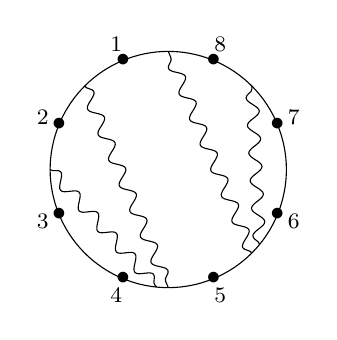
\begin{tikzpicture}[rotate=67.5,baseline=(current bounding box.east)]
	\begin{scope}
	\drawWLD{8}{1.5}
	\drawnumbers
	\drawprop{1}{0}{4}{0}
	\drawprop{2}{0}{4}{-1}
    \drawprop{5}{0}{8}{0}
    \drawprop{5}{1}{7}{0}
		\end{scope}
	\end{tikzpicture} \quad
W_2 = 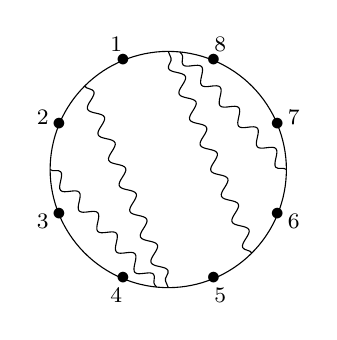
\begin{tikzpicture}[rotate=67.5,baseline=(current bounding box.east)]
	\begin{scope}
	\drawWLD{8}{1.5}
	\drawnumbers
	\drawprop{1}{0}{4}{0}
	\drawprop{2}{0}{4}{-1}
    \drawprop{5}{0}{8}{0}
    \drawprop{6}{0}{8}{-1}
		\end{scope}
	\end{tikzpicture} \quad
W_3 = 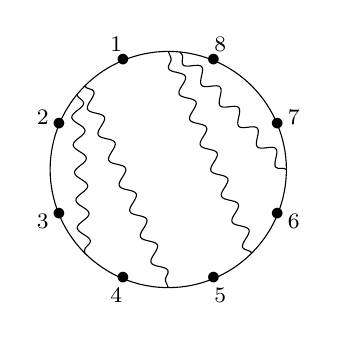
\begin{tikzpicture}[rotate=67.5,baseline=(current bounding box.east)]
	\begin{scope}
	\drawWLD{8}{1.5}
	\drawnumbers
	\drawprop{1}{0}{4}{0}
	\drawprop{1}{1}{3}{0}
    \drawprop{5}{0}{8}{0}
    \drawprop{6}{0}{8}{-1}
		\end{scope}
	\end{tikzpicture} .
\eas


The diagrams $W_1 \sim W_2$ because $(\{(5,8), (5,7)\}, \{5,6,7,8,1\})$ and $(\{(5,8), (7,8)\}, \{5,6,7,8,1\})$ are the corresponding differing subdiagrams. Furthermore, there is the equivalence $W_2 \sim W_3$ due to the exact subdiagrams $(\{(1,4), (3,4)\}, \{1,2,3,4,5\})$ and $(\{(1,4), (1,3)\}, \{1,2,3,4,5\})$. This forces an equivalence between $W_1$ and $W_3$, even though one cannot partition the propagators of each into a an exact subdiagram (that may vary between the diagrams) and a complement that is fixed.  \end{eg}

Each Wilson loop diagram, $W = (\cP, [n])$ with $|\cP| = k$ is associated to a $k \times n$ matrix with non-zero real variable entries, called $C(W)$:

\ba C(W)_{p,q} = \begin{cases} c_{p,q} & \textrm{ if } q \in V(p) \\
0  & \textrm{ if } q \not \in V(p)  \end{cases}
\;. \label{C(W) dfn}\ea

\begin{eg}
For example, ordering the propagators of $W_1$ from Example \ref{eg:equivdiags}: \bas (1,4), \, (2,4), \, (5,7), \, (5,8) \eas we may write
\bas C(W_1) = \left(
\begin{array}{cccccccc}
c_{1,1} & c_{1,2} & 0 & c_{1,4} & c_{1,5} & 0 & 0 & 0 \\
0 & c_{2,2} & c_{2,3} & c_{2,4} & c_{2,5} & 0 & 0 & 0 \\
0 & 0 & 0 & 0 & c_{3,5} & c_{3,6} & c_{3,7} & c_{3,8} \\
c_{4,1} & 0 & 0 & 0 & c_{4,5} & c_{4,6} & 0 & c_{4,8}  \\
\end{array}
\right) \;.\eas

\end{eg}

These $C(W)$ parametrize a subspace of $\Gr(k, n)$ as shown in \cite{wilsonloops}, call it $\Sigma(W)$. The Wilson loop diagrams also define a volume form on $\Sigma(W)$: \bas \Omega(W) = \frac{\prod_{r=1}^{|\cP|} \prod_{v \in V_{p_r}} \textrm{d}c_{p_r}}{R(W)} \;. \eas The denominator $R(W)$ is a polynomial defined by $2 \times 2$ and $1 \times 1$ minors of $C(W)$ as defined below.

\begin{dfn}\label{def R(W)}
For $W = (\cP, [n])$, $R(W) = \prod_{e=1}^n R_e$, with $R_e$ defined by the propagators ending on it. For any edge $e$ of $W$, order the propagators incident on $e$ as $\{p_1 \ldots p_r\}$, ordered such that $p_1$ is closest to the vertex $e$, $p_r$ closest to $e+1$, and $p_i$ is closer to $e$ than $p_{i+1}$. Then \bas R_e =  c_{p_1,e+1} \prod_{j= 1}(r-1) \left((c_{p_j,e} c_{p_{j+1},e+1} - c_{p_{j+1},e} c_{p_{j},e+1} ) \right) c_{p_s,e}\;.\eas Note that in this notation, if $r = 1$, $R_e = c_{p,e} c_{p,e+1}$.
\end{dfn}


\section{Equivalence classes of Wilson loop diagrams}

In \cite{wilsonloop}, Agarwala and Amat show that Wilson loop diagrams can be interpreted as positroids, a certain well behaved class of realizable matroids (this correspondence is stated precisely in Theorem \ref{thm WLD defines matroid} below). This opens up the study of Wilson loop diagrams to techniques from geometry and combinatorics.

In subsection 2.1, we discuss a few matroidal facts about Wilson loop diagrams. In section 2.2, we show that there is a one to one correspondence between exact subdiagrams of Wilson loop diagrams and triangulated pieces of the corresponding polygon partion. In section 2.3, we return to some matroidal facts about Wilson loop diagrams, and exact subdiagrams in partuclar. We show that a subdiagram of $W$ defines a uniform matroid if and only if the subdiagram is exact. This is then used to prove the main result of section 2.3, which is that that two admissible Wilson loop diagrams define the same matroid if and only if they are equivalent (Theorem \ref{same matroid iff equiv}), and we obtain a formula for the number of admissible Wilson loop diagrams in each equivalence class (Corollary \ref{number of equiv diagrams}).  [sentence about why this matters] \todo{much of the above is just text. PUT REFERENCES IN}


\subsection{Wilson loop diagrams as matroids\label{sec matroid background}}

We first give a quick summary of the matroid terminology that we will need; it is not intended as a comprehensive introduction to matroids and the interested reader is referred to [ref][find a good matroid reference].

A {\em matroid} $M = (E,\cB)$ consists of a finite ground set $E$ and a non-empty family $\cB \subseteq \cP(E)$ whose elements satisfy the {\em basis exchange property}: for any distinct $B_1,B_2 \in \cB$ and any $a \in B_1 \setminus B_2$, there exists some $b \in B_2 \setminus B_1$ such that $(B_1 \setminus \{a\})\cup \{b\} \in \cB$ as well. The elements of $\cB$ are called the {\em bases} of the matroid. Note that the basis exchange property immediately implies that all bases have the same size.

A subset $A \subseteq E$ is called {\em independent} in $M$ if $A \subseteq B$ for some $B \in \cB$, and {\em dependent} else. The {\em rank}  $\rk(A)$ of a subset $A \subseteq E$ is the size of the largest independent set contained in $A$. The rank of the matroid itself is defined to be $\rk(E)$.

A {\em circuit} in $M$ is a minimally dependent set. That is, it is a set $C \subseteq E$ such that $C$ is dependent but $C \setminus \{e\}$ is independent for any $e \in C$. A union of circuits is called a {\em cycle}. On the other hand, a {\em flat} is a maximally dependent set, i.e. a set $F \subseteq E$ such that $\rk(F \cup \{e\}) = \rk(F) + 1$ for any $e \in E \setminus F$. Unsurprisingly, a {\em cyclic flat} is a set which is both a flat and a cycle. The set of circuits in a matroid uniquely defines that matroid, as does the set of flats; thus one could specify a matroid by listing its independent sets, bases, circuits, or flats. [ref]

Finally, we describe several important types of matroids. A matroid of rank $k$ with a ground set of size $n$ is called {\em realizable} if there exists some $A \in Gr(k,n)$ whose non-zero $k\times k$ minors are exactly those with columns indexed by elements of $\cB$. A {\em positroid} is a matroid which can be realized by an element of the totally nonnegative Grassmannian $\Gr(k,n)$. Finally, a {\em uniform matroid} of rank $r$ is a matroid in which any set of size $\leq r$ is independent.


Matroid theory relates to the study of Wilson loop diagrams as follows. In \cite{wilsonloop}, Agarwala and Amat show that every admissible Wilson loop diagram with $k$ propagators defines a positroid of rank $k$, and that the independent sets can be read directly from the diagram:

\begin{thm} \label{thm WLD defines matroid} \cite[Theorem 3.6]{wilsonloop} Any admissible Wilson loop diagram $W =(\cP, [n])$ defines a matroid $M(W)$ with ground set $[n]$. The independent sets are exactly those subsets $V \subseteq [n]$ such that $\nexists U\subseteq V$ satisfying $|\Prop(U)| < |U|$. \label{thm:WLDmatroid}\end{thm}
In other words, the independent sets of $M(W)$ correspond to the sets of vertices in $W$ such that no subset supports fewer propagators than the vertices it contains.

Throughout, we take the {\em matroid defined by $W$} to be the matroid $M(W)$ of Theorem \ref{thm WLD defines matroid}. Note that since vertices of the diagram $W$ correspond to columns of the associated matrix $C(W)$, $M(W)$ can also be thought of as the matroid realized by $C(W)$. 


% The identification of Theorem \ref{thm WLD defines matroid} is not 1-1: by \cite[Theorem 1.18]{wilsonloop}, if two admissible Wilson loop diagrams are equivalent (as in Definition~\ref{equivdfn}) then they define the same matroid. 


Let $W = (\cP,n)$ be an admissible Wilson loop diagram, and $M(W)$ its associated matroid. Where it will not cause confusion we conflate the two objects, identifying vertices of $W$ with elements of the ground set $[n]$ in $M(W)$. 

In particular, this allows us to prove results about $M(W)$ by considering the behavior of propagators in $W$. We record a few elementary facts about the rank and cycles of $M(W)$ here as an example of this.

\begin{lem}\label{lem facts about WLD matroids}
Let $W = (\cP,n)$ be an admissible Wilson loop diagram. Then:
\begin{enumerate}
\item The rank of a set $V \subseteq [n]$ is bounded above by $\min\{|V|,|\Prop(V)|\}$, with $\rk(V) = |V|$ if and only if $V$ is an independent set.
%\item Let $v \in [n]$ and $q \in \Prop(v)$. Then for any $V \subset [n]$ such that $q \not \in \Prop(V)$, we have $\rk(V \cup \{v\}) = \rk(V) +1$, i.e. adding a vertex that supports a new propagator to a set increases the rank of the set.
\item If $C \subseteq [n]$ is a cycle, then $\rk(C) = |Prop(C)|$.
\item If $[n]$ can be partitioned into at least two non-empty sets, each of which support different sets of propagators that form a partition of the propagotor set, \bas [n] = \sqcup_i V(P_i) \quad \textrm{s.t.} \quad \sqcup P_i = \cP; \quad V(P_i) \cap V(P_j) = \emptyset; \quad  P_i \cap P_j = \emptyset \;, \eas then the matroid $M(W)$ is seperable, \bas M(W) = \bigoplus_i M(P_i, V(P_i)) \;.\eas 
\item $F(P)$ is a flat of $M(W)$, thus justifying the name ``propagator flat''.
\end{enumerate}
\end{lem}
\begin{proof}
The first part of (1) is \cite[Equation (9)]{wilsonloop} and surrounding discussion, and the second part is standard matroid theory. (2) is \cite[Lemma 3.27]{wilsonloop}. (3) is a direct consequence of \cite[Lemma 3.20]{wilsonloop} and the fact that $F(P_1)^c = V(P_1^c)$

To prove (4), we need to show that $F(P)$ is maximally dependent. If $F(P) = [n]$ then this is automatic, so suppose not and let $v \in [n] \setminus F(P)$. In other words, $v \in V(P^c)$ and so $v$ supports some propagator $q \not\in P$.  Let $S \subseteq F(P)$ be an independent set of maximal size. Then $\Prop(S) \subseteq P$ by (1), and no subset of $S$ supports fewer propagators than the number of vertices it contains (this is the definition of an independent set in $M(W)$). Since $v$ supports a new propagator $q \not\in P$, the set $S \cup \{v\} \subseteq F(P) \cup\{v\}$ also satisfies this independence condition. Thus $\rk(F(P) \cup\{v\}) = \rk(F(P)) + 1$, as required.
\end{proof}

Note that this means that the set $F(\emptyset)$ is the maximal subset of vertices of $W$ of rank $0$. That is, it is the unique flat of rank $0$ in $M(W)$. \sanote{I'm sprinkling comments about $F(\emptyset)$ throughout until we can come up with a better name than unsupportive vertices.}

\subsection{Polygon partitions of Wilson loop diagrams\label{sec: polygon partitions}}


The equivalence relation on Wilson loop diagrams is defined in terms of exact subdiagrams; thus in order to understand the equivalence, we need a way to extract and compare exact subdiagrams. We do this via the notion of a polygon partition of $W$.

\begin{dfn}
  Let $W = (\cP, [n])$ be an admissible Wilson loop diagram.  The \emph{polygon partition} associated to $W$, denoted $\tau(W)$, is defined as follows.
  \begin{itemize}
  \item The vertices of $\tau(W)$ correspond to the edges of $W$.
  \item Labeling the vertices of $\tau(W)$ with the edge number of $W$gives a cyclic order to the vertices. Connecting consecutive vertices gives a graph theoretic cycle called the polygon of $\tau(W)$.
  \item Each propagator of $W$ defines a chord edge of $\tau(W)$; specifically,  a propagator $(i,j) \in \cP$ defines a chord connecting the vertices $i$ and $j$ in $\tau(W)$.
  \end{itemize}
\end{dfn}

\begin{lem}\label{tausimpleplanarlem}
If $W = (\cP, [n])$ is an admissible Wilson loop diagram, then $\tau(W)$ is a simple planar graph whose outer face is a cycle. It is embedded such that the vertices all lie on this infinite face\footnote{That is, it is an \emph{outerplanar} graph}. These vertices are cyclically ordered, with a choice of first vertex giving it an additional compatible linear order.
\end{lem}

\begin{proof}
Since the vertices of $\tau(W)$ are labeled by the edges of $W$, which are cyclically ordered, this gives an ordering to the vertices and the outer face of $\tau(W)$ is a cycle. Since $W$ is admissible, no pairs of propagators cross. Therefore, it is a planar embedding. Similarly, $W$ does not admit any propagators of the form $p = (i, i+1)$; therefore there is exactly one edge connecting any two adjacent edges of $\tau(W)$. Finally, there does not exist two propagators $p,q$ such that both $p$ and $q$ start at edge $i$ and end at edge $j$. Therefore, no other two vertices of $\tau(W)$ can be connected by more than one edge. Finally, the embedding of $\tau(W)$ is induced from the embedding of the graph $W$.
 \end{proof}

\begin{comment}
\hlfix{For an admissible $W$ no propagators cross and so no chord edges of $\tau(W)$ cross.  Thus, in graph theoretic language, we can view $\tau(W)$ as a planar embedding of a
graph with no cut vertices, where all vertices lie on the infinite face, along with a distinguished start vertex and direction around the infinite face.  From this viewpoint the polygon of $tau(W)$ is the boundary of the infinite face.}{I've smushed this together a bit in the prev. lem. Tell me if I've missed anything. Its a lemma for emphasis, not difficulty}
\end{comment}

\begin{eg}\label{WLDtopolygonpartition}
In this example we return to two of the Wilson loop diagrams in Example \ref{eg:equivdiags}. We can pair diagrams with their polygon partitions as follows:
\bas W_1 = 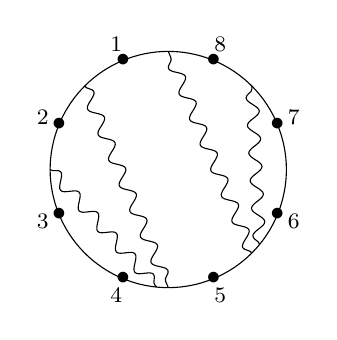
\begin{tikzpicture}[rotate=67.5,baseline=(current bounding box.east)]
	\begin{scope}
	\drawWLD{8}{1.5}
	\drawnumbers
	\drawprop{1}{0}{4}{0}
	\drawprop{2}{0}{4}{-1}
    \drawprop{5}{0}{8}{0}
    \drawprop{5}{1}{7}{0}
		\end{scope}
	\end{tikzpicture} \quad; \quad
\tau(W_1) = 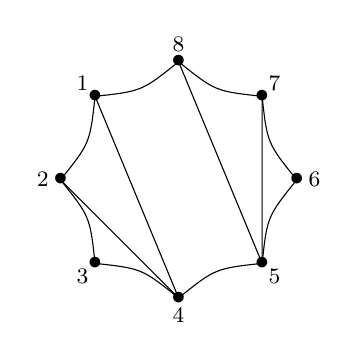
\begin{tikzpicture}[rotate=67.5,baseline=(current bounding box.east)]
	\begin{scope}
	\drawpolypart{8}{1.5}
    \drawnumbersshift
    \drawchord{1}{4}
    \drawchord{2}{4}
    \drawchord{5}{8}
    \drawchord{5}{7}
	\end{scope}
	\end{tikzpicture}
\eas and
\bas W_3 = 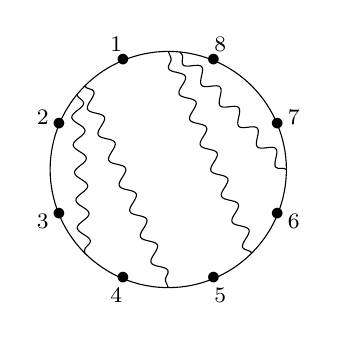
\begin{tikzpicture}[rotate=67.5,baseline=(current bounding box.east)]
	\begin{scope}
	\drawWLD{8}{1.5}
	\drawnumbers
    \drawprop{1}{0}{4}{0}
	\drawprop{1}{1}{3}{0}
    \drawprop{5}{0}{8}{0}
    \drawprop{6}{0}{8}{-1}	
		\end{scope}
	\end{tikzpicture}\quad; \quad
\tau(W_3) = 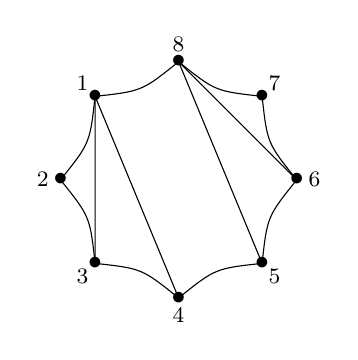
\begin{tikzpicture}[rotate=67.5,baseline=(current bounding box.east)]
	\begin{scope}
	\drawpolypart{8}{1.5}
    \drawnumbersshift
    \drawchord{1}{4}
    \drawchord{1}{3}
    \drawchord{5}{8}
    \drawchord{6}{8}
	\end{scope}
	\end{tikzpicture} .
\eas

\end{eg}

Recall that a planar embedding of a graph is a \emph{triangulation} if all faces, except possibly the infinite face, are triangles.

\begin{dfn}
  Let $W$ be an admissible Wilson loop diagram and $\tau(W)$ its polygon partition. A \emph{triangulated piece} of $\tau(W)$ is a 2-connected subgraph of $\tau(W)$ which is a triangulation. We will take the convention that a subgraph consisting of a single chord edge is called a \emph{trivial} triangulated piece.
A {\em maximal} triangulated piece is one which is not contained in any strictly larger triangulated piece.
\end{dfn}

\begin{dfn}
 A {\em decomposition} of a polygon partition $\tau(W)$ is a set of 2-connected induced subgraphs of $\tau(W)$ which partition the edges of $\tau(W)$.  
\end{dfn}

\begin{eg} \label{eg: unique decomposition} For the Wilson loop diagrams and polygon partitions in Example \ref{WLDtopolygonpartition}, the vertex sets $\{1, 2, 3,4\}$ and $\{5, 6, 7, 8\}$ give maximal triangulated pieces for both $\tau(W_1)$ and $\tau(W_3)$. The vertex set $\{4,5, 8, 1\}$ is not a triangulation in either polygon partition. 
\end{eg}

\begin{lem} \label{decompositionlem}
  For $W$ an admissible Wilson loop diagram, the polygon partition $\tau(W)$ has a unique decomposition into maximal triangulated pieces, and edges in the polygon of $\tau(W)$.
\end{lem}



\begin{proof}
We begin by giving an algorithm for the decomposition, then prove its uniqueness. Let $W = (\cP, [n])$, with $|\cP| = k$.

By \emph{splitting} a vertex $v$ we will mean replacing $v$ by new vertice $v_1, v_2,\ldots, v_{\text{deg}(v)}$ such that each $v_i$ has exactly one neighbour and the union of the of the $v_i$ is the neighbourhood\footnote{The neighbourhood of a vertex is the set of adjacent vertices} of $v$.

Let $T(W)$ be the dual graph of $\tau(W)$ with the vertex corresponding to the infinite face split.
%In other words, place a vertex on each finite face of $\tau(W)$. These vertices are connected if there is a chord edge separating the edges. Furthermore, if the face is bounded by an edge of the polygonal cycle of $\tau(W)$, the corresponding vertex gets a leaf edge for each such boundary.
Since $\tau(W)$ is an embedded graph (with a fixed distinguished embedding) by Lemma \ref{tausimpleplanarlem}, $T(W)$ is an uniquely defined graph.

Furthermore $T(W)$ is a tree because it is connected, has $n+k+1$ vertices ($k+1$ from the internal faces of $\tau(W)$ and $n$ from the outer face) and $n+k$ edges (since $\tau(W)$ has $n+k$ edges).  Additionally, since $\tau(W)$ is simple, $T(W)$ has no vertices of degree $2$.  

%We claim that $T(W)$ is a tree. Since $\tau(W)$ is a planar graph with $k$ chord edges and no internal vertices, there are $k+1$ internal faces of $\tau(W)$. Each of these internal faces corresponds to a vertex of $T(W)$, and there are $n$ vertices of $T(W)$ from the splitting of the dual graph, so $T(W)$ has $n+k+1$ vertices in total. On the other hand, $T(W)$ has $n+k$ edges, corresponding to the $n +k$ edges of $\tau(W)$. Therefore, $T(W)$ is a tree.

Split every vertex of $T(W)$ which has degree $>3$.
%By construction, each face of $\tau(W)$ is a polygon. Therefore, each vertex of $T(W)$ is at least 3 valent (one for each edge of the polygon). \hlfix{If split each vertex of $T(W)$ if it is strictly greater than $3$ valent.}{???} (In other words, we fail to split exactly when the face is a triangle).
The connected components of $T(W)$ correspond to the decomposition of $\tau(W)$ into maximal triangulated pieces and edges originally in the polygon of $\tau(W)$.  Let $f$ be the forest thus obtained.
The vertices of $f$ either have degree 1 or 3.
%, (if they correspond leaf vertices) or 3,  (if they correspond to triangular faces).
Trees of $f$ with no trivalent vertices correspond to either edges in the polygon of $\tau(W)$, if they were originally leaves of $T(W)$, or to maximal trivial triangulated pieces.
Splitting at all the faces that are not triangles ensures maximality of the decomposition. If the splitting were not maximal, then one could add a triangle to a connected component of the splitting, but this would imply that that splitting happened at a valence $3$ vertex.

\bas 
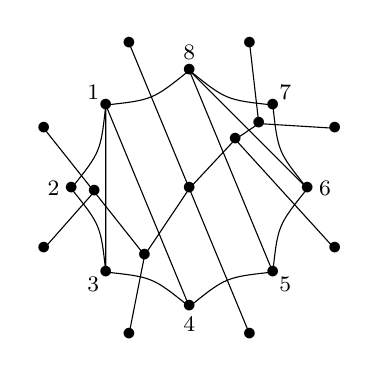
\begin{tikzpicture}[rotate=67.5,baseline=(current bounding box.east)]
	\begin{scope}
	\drawpolypart{8}{1.5}
    \drawnumbersshift
    \drawchord{1}{4}
    \drawchord{1}{3}
    \drawchord{5}{8}
    \drawchord{6}{8}
 \draw (0,0) node {$\bullet$};
\draw (-1,.2) node {$\bullet$};	
\draw (-.5,1.1) node {$\bullet$};
\draw (.8,-.3) node {$\bullet$};	
\draw (1.1,-.5) node {$\bullet$};
\draw(1.1,-.5) -- (.8,-.3) --(0,0)--(-1,.2) -- (-.5,1.1);
\foreach \i in {1,2,...,8} {
      \draw (45*\i:2) node {$\bullet$};
    }
\draw (45*1:2) --(0,0) -- (45*5:2);
\draw (45*6:2) -- (.8,-.3);
\draw (45*8:2) -- (1.1,-.5) -- (45*7:2);
\draw (45*2:2) -- (-.5,1.1) -- (45*3:2);
\draw (45*4:2) -- (-1,.2);
	\end{scope}
	\end{tikzpicture} \rightarrow 
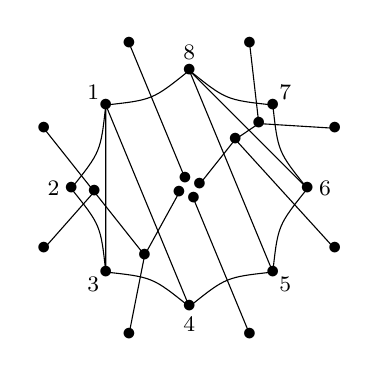
\begin{tikzpicture}[rotate=67.5,baseline=(current bounding box.east)]
	\begin{scope}
	\drawpolypart{8}{1.5}
    \drawnumbersshift
    \drawchord{1}{4}
    \drawchord{1}{3}
    \drawchord{5}{8}
    \drawchord{6}{8}
 \draw (.1,.1) node {$\bullet$};
\draw (.1,-.1) node {$\bullet$};
\draw (-.1,-.1) node {$\bullet$};
\draw (-.1,.1) node {$\bullet$};
\draw (-1,.2) node {$\bullet$};	
\draw (-.5,1.1) node {$\bullet$};
\draw (.8,-.3) node {$\bullet$};	
\draw (1.1,-.5) node {$\bullet$};
\draw(1.1,-.5) -- (.8,-.3) --(.1,-.1); 
\draw (-.1, .1) --(-1,.2) -- (-.5,1.1);
\foreach \i in {1,2,...,8} {
      \draw (45*\i:2) node {$\bullet$};
    }
\draw (45*1:2) --(.1,.1);
\draw (-.1, -.1) -- (45*5:2);
\draw (45*6:2) -- (.8,-.3);
\draw (45*8:2) -- (1.1,-.5) -- (45*7:2);
\draw (45*2:2) -- (-.5,1.1) -- (45*3:2);
\draw (45*4:2) -- (-1,.2);
	\end{scope}
	\end{tikzpicture}
\eas



To see uniqueness, consider a different maximal decomposition of $\tau(W)$. This induces a splitting on $T(W)$, where each connected component of the new decomposition corresponds to a subtree. Call this forest $f'$. Since $f' \neq f$, there are two trees, $t$ and $t'$ in $f$ and $f'$ that are distinct, but share at least one edge of $T(W)$. Since $f'$ is also maximal, $t'$ is not a subtree of $t$. Therefore, the edges of $t'$ can be found in at least two trees in the forest $f$. In particular, there is a vertex $v$ in $t'$ that corresponds to a split vertex of $T(W)$ in the original decomposition.
This implies that $v$ has valence greater than $3$ in $T(W)$, and thus the corresponding face of $\tau(W)$ is not a triangle. In other words, the decomposition corresponding to $f'$ is not a triangulation. 
\end{proof}

\begin{cor} \label{maxtriangdisjointcor}
Given a maximal decomposition of $\tau(W)$, the maximal triangulated pieces are edge disjoint.
\end{cor}

\begin{proof}
Consider any two distinct maximal triangulated pieces of $\tau(W)$. These two pieces correspond to subtrees of $T(W)$ and intersect, at most, at a vertex in the interior of $\tau(W)$. Since the subtrees corresponding to the maximal triangulated pieces are edge disjoint, and the edges of $T(W)$ correspond to the edges of $\tau(W)$, this forces the maximal triangulated pieces to be edge disjoint as well.
\end{proof}


We are now in a position to relate the triangulated pieces of $\tau(W)$ to exact subdiagrams of $W$.

Every triangulated piece $t$ of an admissible Wilson loop diagram $W$ corresponds to a subdiagram of $W$ by taking the set of propagators $P$ corresponding to edges of $t$ and then taking the subdiagram $W_P = (P, V(P))$.  Conversely, given a subdiagram $W_P = (P, V(P))$ of $W$ we can obtain a subgraph of $\tau(W)$, called $t$, as follows:
\begin{itemize}
\item The vertex set of the subgraph $t$ is
  \begin{itemize}
  \item the vertices of $\tau(W)$ corresponding to edges of $W$ defined by cyclically consecutive elements of $V(P)$ as a subset of $[n]$
  \end{itemize}
\item The edge set of the subgraph is
  \begin{itemize}
  \item the edges of $\tau(W)$ corresponding to propagators of $P$
  \item along with the outer edges of $\tau(W)$ for which both their end points are in the vertex set
  \end{itemize}
\end{itemize}
Note that the subgraph $t$ depends on how the propagators of $P$ sit inside $[n]$, not on how they sit in $W_P$ itself.  In particular $t$ is not the subgraph of $\tau(W)$ consisting only of edges corresponding to propagators of $P$. 


\begin{lem}\label{lem triang to exact}
  Let $W$ be an admissible Wilson loop diagram and $\tau(W)$ its polygon partition.  The triangulated pieces of $\tau(W)$ correspond to the exact subdiagrams of $W$ using the correspondence described above.
\end{lem}

\begin{proof}
Let us first record a few standard facts about polygon triangulations (that is, about triangulations with all vertices on the outer face).  If such a triangulation has $n$ vertices then it has $n$ edges on the polygon (that is, on the outer face) and $n-3$ edges which are not.  No planar graph with the same vertices and the same outer face can have more edges than the triangulation, and every such simple graph with $n-3$ edges off the outer face is a triangulation.

Since $W$ is admissible, by Lemma \ref{tausimpleplanarlem} $\tau(W)$ is a simple graph. Let $t$ be a triangulated piece of the decomposition of $\tau(W)$ given in Lemma \ref{decompositionlem}; note that $t$ cannot be equal to $\tau(W)$ by the definition of admissible diagrams.

If $t$ has 2 vertices then $t$ corresponds to a propagator that connects two non-adjacent edges. Therefore, the trivial triangulation is a trivial exact subdiagram.

Now suppose that $t$ has $m>2$ vertices.  We count how many edges of $t$ are not on the outer face of $\tau(W)$.  These are exactly the edges of $t$ defined by propagators of $W$. Consider the intersection of $t$ with the outer face of $\tau(W)$: this is a possibly disconnected subgraph of the polygon of $\tau(W)$ and this subgraph has $m$ vertices. Call this new subgraph $S$, and let $j$ be the number of connected components of $S$.   To join the components of $S$ into the outer face of $t$, $t$ must have $j$ edges in its outer face which are not in the outer face of $\tau(W)$.  Furthermore $t$ has $m-3$ edges not in its outer face and so also not in the outer face of $\tau(W)$.  Thus there are $m-3+j$ edges of $t$ not in the outer face of $\tau(W)$.

Each of these $m-3+j$ internal edges corresponds to a propagator in $W$; call this set of propagators $P$.  Next we count the size of $V(P)$.  Each of the $m$ vertices in the outer face of $t$ corresponds to an edge of $W$. These $m$ edges define $j$ connected components of the outer polygon of $W$. Thus the set $V(P)$ has $m+j$ vertices.  In other words, 
\[|V(P)| = m+j = |P| +3\;.\]
Thus the subdiagram $(P,V(P))$ defined by $t$ is exact.


Conversely, suppose we have an exact subdiagram $(P, V(P))$ of $W = (\cP, [n])$ supported on $|V(P)| = |P|+3$ vertices, and let $t$ be the subgraph of $\tau(W)$ corresponding to $(P,V(P))$.

Suppose $|P|=1$. Let $p$ be the element of $P$. The exactness condition on $(P, V(P))$ says that the four supporting vertices of $p$ are distinct.  If the support of $p$ is four consecutive vertices, then $V(p)$ defines three consecutive boundary edges of $W$, so $t$ is a single triangle, hence a triangulated piece.  If the support of $p$ is not four consecutive vertices, then the vertices which are the ends of $t$ are separated by at least two vertices along the cycle.  This implies that $t$ is a trivial triangulated piece.

Now suppose $|P|>1$.  Let $j=|P|$, $m=|V(P)|$, and 
suppose that the set $V(P)$ defines $c$ disjoint cyclic intervals of $[n]$. Then $t$ has $m-c$ vertices.  If $t$ were a triangulation, $t$ would have $j -c$ internal edges.

The graph $t$ has $j$ edges that come from propagators, and $m - 2c$ edges that come from the boundary polygon of $\tau(W)$. Since $t$ has $m-c$ vertices, it has $m-c$ external edges, of which $c$ come from propagators. Therefore, of the $j$ edges of $t$ that come from propagators, $j-c$ are internal to the connected component. Therefore, $t$ is a triangulated piece.


%  The statement of the lemma then follows form the fact that inclusion is preserved under $\tau$ and so maximality also corresponds under $\tau$.
\end{proof}





To avoid the issue of exact diagrams being subdiagrams of other exact subdiagrams (for instance, any subdiagram $(q, V(q))$, for $q \in \cP$ is exact), we introduce the notion of maximal exact subdiagrams.

\begin{dfn}
An exact subdiagram $(P, V(P))$ is a {\em maximal exact subdiagram} of $W$ if there is no other exact subdiagram $(Q, V(Q))$ in $W$ that contains $(P,V(P))$ as a strict subdiagram.
\end{dfn}


\begin{cor} \label{uniqueproppartitioncor}
Any admissible Wilson loop diagram $W = (\cP, [n])$ can be uniquely decomposed into maximal exact subdiagrams. These maximal subdiagrams partition $\cP$.
\end{cor}

\begin{proof}
Combining Lemmas \ref{decompositionlem} and \ref{lem triang to exact} yields the unique decomposition into maximal exact subdiagrams, and Corollary \ref{maxtriangdisjointcor} ensures that no propagator appears in more than one subdiagram in this decomposition. Since the chord edges of $\tau(W)$ correspond to the propagators of $W$, the decomposition of $\tau(W)$ induces a partition of $\cP$.
\end{proof}

\subsection{Matroidal properties of exact subdiagrams \label{sec: exact diagram matroidal props}}

Since Corollary \ref{uniqueproppartitioncor} allows us to decompose any admissible Wilson loop diagram into a collection of maximal exact subdiagrams, in this section we examine the matroid properties of exact subdiagrams more closely. In particular, we show that given an exact subdiagram $(P, V(P))$, it can be written as the contraction of the matroid $M(W)$ by the complementary propagator flat, $F(P^c)$. Furthermore, if $(P, V(P))$ is a maximal exact subdiagrams, its complementary propagator flat is a cyclic flat. Finally, we show that matroids associated to exact subdiagrams are uniform (Theorem \ref{exactuniformthm}). 

We begin by proving some useful facts about flats of matroids associated to admissible Wilson loop diagrams.

\begin{comment}

\begin{dfn}\label{matroid contraction}
Let $M = (E,\cB)$ be a matroid, and $S \subseteq E$. The {\em contraction} of $M$ by $S$ is the matroid $M/S = (E \setminus S, \cB / S)$, where
\[\cB / S = \{B \setminus S \ \big| \ |B\cap S | \text{ is maximal amonst all }B \in \cB\}.\]
\end{dfn}



In \cite{wilsonloop}, Agarwala and Amat show that certain subdiagrams of $W$ can be realized as contractions of $M(W)$:

\begin{lem} \label{contractsubdiaglem} \cite[Theorem 3.33]{wilsonloop} 
Let $W = (\cP, [n])$ be an admissible Wilson loop diagram and $P \subseteq \cP$. If the set $V(P)^c$ has rank $|P^c|$, then the matroid defined by the subdiagram $(P, V(P))$ is equal to the contraction $M(W)/V(P)^c$.
\end{lem}


In Lemma \ref{maxexactcomplementrank} below we show that every exact subdiagram satisfies the rank condition of Lemma \ref{contractsubdiaglem}. In order to do this, we first examine the properties of the set by which we contract.

\begin{dfn}\label{def prop flat} 
Let $W = (\cP,[n])$ be an admissible Wilson loop diagram and $P \subseteq \cP$. The set $F(P) := V(P^c)^c$ is called the {\em propagator flat} of $P$.
\end{dfn}
Thus in Lemma \ref{contractsubdiaglem} above we would contract $M(W)$ by the propagator flat $F(P^c)$ of the {\em complement} of $P$ in order to study $(P,V(P))$. The justification for this notation is given by (1) of the next lemma: the set $F(P)$ consists of vertices which {\em only} support propagators in $P$ (or no propagators at all).

\begin{lem}\label{lem properties of prop flats} \sanote{do we need the first 2? They follow directly from the definition 1.2. Do we use them later?}
Let $F(P)$ be a propagator flat as defined above. Then
\begin{enumerate}
\item $F(\emptyset)$ is exactly the set of vertices which support no propagators, while for $P \neq \emptyset$ we have \[F(P) = \big(V(P) \setminus V(P^c)\big) \cup F(\emptyset).\] \note{updated (1) to match new definition of $F(P)$; }
\item If $Q\subseteq P$ then $F(Q) \subseteq F(P)$.
\item $F(P)$ is a flat of $M(W)$, thus justifying the name ``propagator flat''.
\end{enumerate}
\end{lem} \sanote{I'd like to attach this to the "generic facts about matroids" in lemma 2.2?}
\begin{proof}
The proof of (1) and (2) are routine applications of the definition and are omitted.

To prove (3), we need to show that $F(P)$ is maximally dependent. If $F(P) = [n]$ then this is automatic, so suppose not and let $v \in [n] \setminus F(P)$. In other words, $v \in V(P^c)$ and so $v$ supports some propagator $q \not\in P$.  Let $S \subseteq F(P)$ be an independent set of maximal size. Then $\Prop(S) \subseteq P$ by (1), and no subset of $S$ supports fewer propagators than the number of vertices it contains (this is the definition of an independent set in $M(W)$). Since $v$ supports a new propagator $q \not\in P$, the set $S \cup \{v\} \subseteq F(P) \cup\{v\}$ also satisfies this independence condition. Thus $\rk(F(P) \cup\{v\}) = \rk(F(P)) + 1$, as required.
\end{proof}


\end{comment}

\begin{lem} \label{lem decompose flat}Let $F$ be a flat in $M(W)$, and let $C \subseteq F$ be the union of all circuits contained in $F$. Then the following are true:
\begin{enumerate}
\item $C = F(\Prop (C))$, i.e. $C$ is a propagator flat.
\item $F \setminus C$ is an independent  flat.  
\end{enumerate}
\end{lem}

\begin{proof}
(1) If $F$ is an independent flat, then $C = \emptyset$ and the statement is trivially true. Now suppose that $F$ is a dependent set, so $C$ is non-empty.

Let $v \in C$. Clearly $\Prop(v) \subseteq \Prop(C)$. Since $F(P)  = V(P^c)^c$, we have $F(\Prop(v)) \subseteq F(\Prop(C))$. Since $v \in F(\Prop(v))$ by the definition of propagator flat, we have $v \in F(\Prop(C))$ as required, and $C \subseteq F(\Prop(C))$. 

Now suppose there exists some $w \in  F(\Prop(C)) \setminus C$. Let $B$ be an independent subset of $C$ of maximal rank; we first show that $B \cup \{w\}$ is a dependent set in $M(W)$. By Lemma \ref{lem facts about WLD matroids}, \bas |\Prop(C)| = \rk(C) = |B| = \rk(B) .\eas Since $B \subseteq C$ implies that  $\Prop(B) \subseteq \Prop(C)$, this implies that $\Prop(B) = \Prop(C)$. Furthermore, since $w \in F(Prop(C)$, $\Prop(B\cup w) \subseteq \Prop(B)$. By Lemma \ref{lem facts about WLD matroids} $\rk (B \cup w) \leq \min\{|B\cup w|, |\Prop(B\cup w)|\}$, and therefore $\rk (B \cup w) < |B\cup w|$. That is, $B\cup w$ is a circuit in $F(\Prop(C))$. Therefore, $B \cup w \subset C$, leading to a contradiction.


For part (2), first note that $F \setminus C$ is automatically independent as it contains no circuits.

\note{the one element could be e so this doesn't work}
For any $e \not\in F$, we certainly have $\rk((F\setminus C)\cup\{e\}) = \rk(F\setminus C) +1$ since $F$ is a flat. Now let $e \in C$, and suppose that $\rk((F\setminus C)\cup\{e\}) = \rk(F\setminus C)$. This implies that $(F\setminus C)\cup \{e\}$ is dependent, and hence contains a circuit, $S$. This circuit must contain at least one element but this contradicts the fact that $C$ was the union of all circuits in $F$. 

Thus $\rk((F\setminus C)\cup \{e\}) = \rk(F\setminus C) + 1$ for any $e \not\in F\setminus C$, and hence $F\setminus C$ is a flat.
\end{proof}

\begin{cor} \label{classifyflats}
If $F$ is a flat of a Wilson loop diagram, it can be written as the disjoint union of a cyclic propagator flat and an independent flat. \end{cor}

In particular, any propagator flat can be written as a union of a cyclic propagator flat and an independent flat.

%Finally, we note the differences between subdiagrams of Wilson loop diagrams, and restrictions or cotractions of the associated matroids.

%Given any matroid, one may restrict it to a subset of the base set. The bases of the restricted matroid come from intersecting bases of the original with the subset. It is worth noting that a the matroid defined by a subdiagram is different from the restriction of the matroid of a Wilson loop diagram to a set of vertices.

% \begin{dfn} \label{restrictiondfn}
% For $W = (\cP, [n])$, the restricted diagram, $W|_V$ is the matroid defined by only looking at the vertices $V \subset [n]$.
% \end{dfn}

% The key difference between a subdiagram and a restriction is that the propagator support function does not change in the case of restriction, while it may in the case of a subdiagram. In particular, for $v \in V$, $\Prop_W(v) = \Prop_{W|_V}(v)$, while $\Prop_{(P, V(P))} (v) = \Prop_W(v) \cap P$.

% A subdiagram is more closely related to a contracted matroid.



\begin{lem} \label{maxexactcomplementrank}
Let $W = (\cP, [n])$ be a Wilson loop diagram, and $P \subseteq \cP$. Then: \begin{enumerate}
\item If $(P,V(P))$ is an exact subdiagram in $W$, then $\rk(F(P^c)) = |P^c|$.
\item If $(P,V(P))$ is a maximal exact subdiagram in $W$, then $F(P^c)$ is a cyclic flat.
\end{enumerate}
\end{lem}

Note that $|P^c|$ is always an upper bound on the rank of $F(P^c)$ for any $P \subseteq \cP$, since $F(P^c)$ supports at most $P^c$ propagators. However, showing equality is far harder.

\begin{proof}
First note that if $(P,V(P))$ is exact then the admissiblity of $W$ guarantees that $F(P^c)$ is non-empty. 

Since $W$ is admissible, we have $n \geq |\cP| + 4$. Rewriting this as
\[|V(P)| + |F(P^c)|  \geq  |P| + |P^c| +4,\]
and combining it with the fact that $|V(P)| = |P| + 3$ (from the exactness of $(P,V(P))$), we obtain
\begin{equation}\label{eq F is dependent}|F(P^c)| > |P^c| \;.\end{equation}
By Lemma \ref{lem properties of prop flats}, $F(P^c)$ is a set of vertices that supports only propagators in $P^c$, so in particular we have $\Prop(F(P^c)) = P^c$. Equation \eqref{eq F is dependent} is therefore saying that $F(P^c)$ supports fewer propagators than the number of vertices it contains, i.e. $F(P^c)$ is dependent. 

We address part (2) first. Suppose that $(P, V(P))$ is a maximal exact subdiagram; by Corollary \ref{classifyflats} we can decompose $F(P^c)$ as
\begin{equation}\label{eq decompose F}F(P^c) = C \sqcup S,\end{equation}
where $C$ is the largest cyclic flat contained in $F(P^c)$ and $S$ is an  independent set. Note that $C$ must be non-empty since $F(P^c)$ is non-empty and dependent. We proceed by showing that $S$ must be empty, forcing $F(P^c)$ to be a cyclic flat.

Since $C = F(\Prop(C))$ by Lemma \ref{lem decompose flat}, define $Q := \Prop(C)^c$ so that we may write $C = F(Q^c) = V(Q)^c$. Note that since $C \subseteq F(P^c)$, $P \subseteq Q$. Furthermore, we have 
\begin{equation}|S| = \rk(S) \leq \rk(F(P^c)) - \rk(C)  \leq |P^c| - \rk(C) \;, \label{increasingrank}\end{equation}
where first equality comes from the fact that $S$ is an independent set,\note{Did we ever address the question of where the middle inequality comes from? Can we argue by number of propagators?} and the final inequality comes from Lemma \ref{lem facts about WLD matroids}(1). Since $\rk(C) = |\Prop(C)| = |Q^c|$ by Lemma \ref{lem facts about WLD matroids}(2), we can rearrange \eqref{increasingrank} to obtain the inequality
\begin{equation} |P| + |S| \leq |P| + |P^c| - \rk(C) = |Q| \;. \label{Qsizebound}\end{equation}
Furthermore, since $V(Q) = S \sqcup V(P)$ (by equation \eqref{eq decompose F} and the definition of $Q$) we may write  
\begin{equation} |V(Q)| = |S| + |V(P)| = |S| + |P| +3 \label{VQsize} \;.\end{equation} 
Combining this with \eqref{Qsizebound} gives $|V(Q)| \leq |Q| + 3$. Since $W$ is admissible, we conclude that $(Q,V(Q))$ is exact; since $V(Q) = V(P) \sqcup S$ and $(P,V(P))$ is maximal exact, it follows that $S = \emptyset$. It now follows from \eqref{eq decompose F} that $F(P^c)$ is a cyclic flat, and hence from Lemma \ref{lem facts about WLD matroids} that
\[\rk(F(P^c)) = |Prop(F(P^c))| = |P^c|.\]

Let $P$ be a maximal exact subdiagram as above, and let $(R,V(R))$ be an exact subdiagram that is not maximal. That is, $R \subsetneq P$.

Since $R \subset P$, $V(P) = V(R) \sqcup S$. Since $P$ and $R$ both define exact subdiagrams, we may write $|V(P)| = |V(R)| + |P \setminus R|$, where $S$ is a vertex set of size $|P \setminus R|$ with $(P \setminus R \subset \Prop(S)$. Since $\rk V(P) =  \rk V(R) + |P \setminus R|$, $S$ is independent. Taking the complements, we may write \bas F(R^c ) = F(P^c) \sqcup S \;.\eas Since $S$ is an independent set of vertices of the correct size supporting the appropriate propagators, this gives $ \rk F(R^c ) = |R^c|$.

\end{proof}


In particular, any exact subdiagram $(P,V(P))$ satisfies the conditions of Lemma \ref{contractsubdiaglem} and can therefore be written as a contraction of $M(W)$ by the complementary propagator flat $F(P^c)$. 

Matroids coming from exact subdiagrams have an especially nice structure, as we now show. Recall from Section \ref{sec matroid background} that a uniform matroid of rank $r$ is one in which all sets of size $ \leq r$ are independent.

\begin{thm} \label{exactuniformthm}
Let $W':= (P, V(P))$ be a subdiagram of an admissible Wilson loop diagram $W= (\cP, [n])$. Then $W'$ is an exact subdiagram if and only if $M(W')$ is a uniform matroid of rank $|P|$.
\end{thm}

\begin{proof}
It follows directly from the definitions that a matroid of rank $r$ is uniform if and only if all circuits have rank $r$; we therefore focus on the circuits of $M(W')$.

We prove the following claim: $W'$ is exact if and only if $V(P)$ contains no circuits $C$ with $\rk C< |P|$ in $(P, V(P))$. Since $\rk(M(W')$ is bounded above by $|P|$, the result follows.

Suppose $C \subseteq V(P)$ is a circuit of rank $m < |P|$; by Lemma \ref{lem facts about WLD matroids}, we know that $|\Prop_{W'}(C)| = m$ as well, where the subscript to $\Prop$ specifies the diagram we are working in.  Observe that $\Prop_{W'}(C)\subseteq P$ by definition. The set $P \setminus \Prop_{W'}(C)$ is thus nonempty, and we can consider the subdiagram $W'':= (P\setminus \Prop_{W'}(C),V(P\setminus\Prop_{W'}(C))$. By the density condition on subdiagrams of admissible diagrams, we have
\[|V(P\setminus\Prop_{W'}(C))| \geq |P\setminus\Prop_{W'}(C)| + 3.\]
It is easy to verify that $V(P\setminus\Prop_{W'}(C)) \subseteq V(P)\setminus C$; since $C \subseteq V(P)$ and $\Prop_{W'}(C) \subseteq P$, we can therefore rewrite the previous inequality as
\[|V(P)| - (m+1) \geq |V(P\setminus\Prop(C))| \geq |P| - m + 3.\]
Simplifying, we obtain $|V(P)| \geq |P| + 4$, i.e. $(P,V(P))$ is not an exact diagram.

Conversely, suppose that $W'$ is not exact and for a contradiction suppose also that $M(W')$ is uniform of rank $|P|$.  Take $p \in P$.  Then $|V(P)\setminus V(p)| = |V(P)| - 4 \geq |P|$ by non-exactness.  By uniformity there is an independent set of size $|P|$ in $V(P)\setminus V(p)$.  This is impossible because the submatrix corresponding to this independent set has $|P|$ rows but the one corresponding to $p$ is all $0$ one of them is all 0 so it cannot be full rank.
%suppose that $(P,V(P))$ is not exact, i.e. $|V(P)| \geq |P| +4$. We have 
%\[|V(P)| - (m+1) \geq |P| - m + 3\]
%as above, but \hlfix{we need to know that $P\setminus\Prop(C)$ is non-empty before we can complete the argument.}{and if we knew this, it would be immediate that $\rk(C) < |P|$}
\end{proof}

Before proving the main theorems of this section, we make a few observations about the geometry of matroids defined by exact diagrams.

In \cite{wilsonloops}, the authors show that all violet Wilson loop diagrams correspond to positroids. That is, they correspond to matroids that can be represented by elements of the positive Grassmannians $\Gr(|\cP|, |V|)$. Any positroid of rank $k$ on $n$ elements defines a subspace of the positive Grassmannians $\Gr(k, n)$, namely the points which represent it. These subspaces give a CW structure on $\Gr(k,n)$, with each positroid defining a cell. 

\begin{dfn}
Given a Wilson loop diagram $W = (\cP, [n])$, define the positroid cell associated to a Wilson loop diagram, $\Sigma(W)$, to be the cell in the CW complex on $\Gr(|\cP|, n)$ defined by the positroid $M(W)$.
\end{dfn}

With this definition in mind, we have the following corollary:

\begin{cor}
Let $(P, V(P))$ be an exact subdiagram of $W$. The matroid associated to this subdiagram corresponds to the top dimensional cell in $\Gr(|P|, |V(P)|)$.
\end{cor}

\begin{proof}
The unique top dimensional cell of $\Gr(|P|, |V(P)|)$ is defined by all points in $\Gr(|P|, |V(P)|)$ such that all Plucker coordinates are strictly greater than $0$. Since $(P, V(P))$ is an exact subdiagram, this all $|P| \times |P|$ minors are non-zero. Intersecting these with the cases with the positive Grassmannians demands that all minors be strictly positive.
\end{proof}

%Since the matroid defined by the subdiagram $(P , V(P))$ is not the same as the matroid associated to $W_{V(P)}$, one cannot say that the $W_{V(P)}$ is a uniform matroid. In fact, for any subset $U \subset V(P)$, $\rk_{W_{V(P)}}(U) \geq \rk_{(P , V(P))}(U)$. This is because adding propagators to vertices can only increase the rank. In particular this implies that, for any subset $U \subset V(P)$, if $|U| \leq |P|$, then $U$ is independent in both the restricted matroid $W_{V(P)}$, and the original, $W$.



\subsection{Matroids and equivalent diagrams}
\note{Si\^an postponed reading this section until the earlier ones are fixed.}
Now we are ready to prove the main results of this section, namely that two Wilson loop diagrams define the same matroid if and only if they are equivalent (Theorem [ref]) and a formula for the number of Wilson loop diagrams in a given equivalence class (Corollary [ref]).

\begin{thm}\label{same matroid iff equiv}
Let $W= (\cP, [n])$ and $W'= (\cP', [n])$ be two Wilson Loop diagrams. They define the same matroid if and only if $W \sim W'$.
\end{thm}

\begin{proof}
One direction has been proved in previous work, but we give a different proof here to be consistent with the method of this document.

Assume that $W$ and $W'$ are equivalent. Without loss of generality, write $W = (P \cup R, [n])$ and $W' = (P \cup R', [n])$, where $P \subset \cP \cap \cP'$ and $(R, V(R))$ and $(R', V(R'))$ are two maximally exact subdiagrams, with $R \neq R'$, but $V(R) = V(R')$. If this is not the case, one may always find a family of diagram, $\{W_i\}$ satisfying this condition and forming a transitive chain connecting $W$ to $W'$ in the equivalence class.

Let $U \subset V(R)$ be any subset of size $|U| = |R|$. The set $U$ is independent in the subdiagram $(R, V(R))$, and thus in $W$. The complementary set $F(P)$ is a flat of maximal rank by lemma \ref{maxexactcomplementrank} ($\rk(F(P)) = |P|$). Let $B \subset F(P)$ be a maximal indpendent set ($\rk B = |P|$) in $F(P)$. Since $F(P)$ is a flat, adding any element of $V(R)$ to $B$ increases the rank. Therefore, any basis of $W$ can be written as $B \cup U$. However, since $F(P)$ is common to both $W$ and $W'$, and $V(R) = V(R')$, any any basis of $W'$ can also be written $B \cup U$. Thus both matroids have the same bases sets, proving that they are the same.

For the converse, assume that the matroids associated to $W$ and $W'$ are the same: $M(W) = M(W')= M$. Let $\{(P_i, V(P_i)\}_{i=1}^k$ and $\{(P'_i, V(P'_i)\}_{i=1}^l$ be the sets of maximally exact subdiagrams of $W$ and $W'$. Write $F_i = F(P_i)$ and $F'_i = F(P^{'c}_i)$ to be the complementary cyclic flats. By Lemma \ref{exactcircuitlem} $M/F_i$ is a uniform matroid. Thereofore, $k = l$, and we may write $V(P_i) = V(P'_i)$.

Reorganize the vertex sets as follows: \ba \cup_{P_i \neq P_i'} V(P_i) = V(\cup_{P_i \neq P'_i} P_i)  \label{vertexsets}\; .\ea Since maximal exact subdiagrams partition $\cP$, by Lemma \ref{uniqueproppartitioncor}, write $cup_{i = 1}^k P_i = \cup_{i = 1}^k P'_i = \cP$. Then equation \eqref{vertexsets} becomes \bas \cap_{P_i \neq P_i'} (F(P_i^c))^c = F(\cup_{P_j = P'_j} P_j)^c \;.\eas These flats may, of course, be empty.

Thus, we have partitioned the vertices of $W$ and $W'$ into a single set that supports a union of maximal exact subdiagrams whose propagators between $W$ and $W'$, and the complementary propagator flats that support the propagators in common between $W$ and $W'$. As mentioned above, the latter may be empty.

Define a family of Wilson loop diagrams, $W_0$ to $W_k$ defined such that $W_0 = W$ and $W_i$ is derived from $W_{i-1}$ by replacing the propagator set $P_i$ with $P'_i$. In this manner, $W' = W_k$ and $W_i \sim W_{i+1}$, making $W \sim W'$.
\end{proof}

Since there is a unique way to decompose $W$ into maximal exact subdiagrams, it is logical to ask how many diagrams there are in an equivalence class. It is a classical fact the the number of triangulations of an $n$-gon is the $n-2$ Catalan number, namely $\frac{1}{n-1}\binom{2(n-2)}{n-2}$.  Thus we can count the number of equivalent diagrams.

\begin{cor}\label{number of equiv diagrams}
  Let $W$ be an admissible Wilson loop diagram where the sizes of the supports of the nontrivial maximal connected exact subdiagrams are $n_1, n_2, \ldots, n_j$.  Then the number of admissible Wilson loop diagrams equivalent to $W$ (including $W$ itself) is
  \[
  \prod_{i=1}^{j} \frac{1}{n_i-1}\binom{2(n_i-2)}{n_i-2}
  \]
\end{cor}



\begin{comment}
\subsection{Counting exact subdiagrams}


\begin{dfn}
  Say two admissible Wilson loop diagrams $W_1$ and $W_2$ are \emph{triangulation-equivalent} if there is a bijection $\alpha$ between the set of triangulated pieces in the decomposition of $\tau(W_1)$ and the set of triangulated pieces in the decomposition of $\tau(W_2)$, where $t$ and $\alpha(t)$ have the same vertex set for all triangulated pieces $t$ of $\tau(W_1)$.
\end{dfn}

***draw an example***

\begin{thm}
  Two admissible Wilson loop diagrams have the same matroid iff they are triangulation equivalent
\end{thm}

Again do I want matroid or positroid in this theorem?

\begin{proof}
  By Lemma~\ref{lem triang to exact} two admissible Wilson loop diagrams are triangulation equivalent iff their decompositions into maximal connected exact subdiagrams have matching supports, that is if they are equivalent.
  Theorem~\ref{thm orig equiv} then gives the result.
\end{proof}



\end{comment}

\section{Geometry of Wilson Loop diagram}\label{sec GN algorithm}
Since Wilson loop diagrams correspond to positroids, it is natural to study the subspace of $\Gr(|\cP|, n)$ they define.

Talk about Grassmann Necklaces and how it defines a cell in a CW complex of $\Gr(k,n)$. Also talk about how this is exactly all the non-negative matrices that represent a particular positroid.

Also talk about Le diagrams.

Throughout this section, $W = (\cP,n)$ is an admissible Wilson loop diagram with $k$ propagators.

\subsection{Some setup results about propagators}


%\note{I don't think rank of a vertex (in the sense of number of propagators supported on it) was ever used, so I removed the definition}
%\note{rank probably isn't a good word; do we have a better one?}
%\begin{dfn}\label{vertex rank}
%Let $i$ be a vertex in $W$. We define the {\bf rank} of $i$ to be $|Prop(i)|$, i.e. the number of propagators supported on $i$.
%\end{dfn}




\begin{dfn}\label{props inside p}
Let $p$ be a propagator supported on $(i,j)$ in $W$. The region bounded by $p$ and the edge of the Wilson loop diagram from $i$ to $j+1$ is refered to as the region {\bf inside} $p$, and the complement is the region {\bf outside }$p$. The set of propagators inside (resp. outside) $p$ are those lying in the region inside (resp. outside) $p$, excluding $p$ itself.
\end{dfn}
Note that this depends on the order of $i$ and $j$: if we view $p$ as supported on $(j,i)$ (for example, if we are working with the $<_j$ order on vertices) then the regions inside and outside $p$ are swapped.


\begin{dfn}\note{right now this doesn't depend on the order of $i$ and $j$, but that might matter later on?}
Let $p$ be a propagator supported on $(i,j)$.  Define the \textit{length} of $p$ to be 
\[\ell(p) = min\big\{|[i+1,j]|,|[j+1,i]|\big\}.\]
\end{dfn}




\begin{rmk}\label{rem:props of length 2 and 3}
The following observations about propagators of short length in $W$ are easily verified:
\begin{itemize}
\item If every vertex in $W$ supports at least one propagator, then $W$ admits at least one propagator of length 2.
\item If $p = (i,i+3)$ is a propagator of length 3, then the middle vertex $i+2$ supports at most one propagator.
\end{itemize}
\end{rmk}


The following lemma establishes certain configurations of propagators that must exist in any admissible diagram with no unsupported vertices. We make use of this result in several induction proofs below.

\begin{lem}\label{lem sian}
  Let $W$ be a weakly admissible WLD with at least 5 vertices and in which each vertex supports at least one propagator.  Then at least one of the following two things occurs.
  \begin{enumerate}
    \item $W$ has a propagator of length $\leq 6$ with a propagator of length 2 inside it and nothing else inside it.\label{item big and 2}
    \item There exists a pair of propagators of length $2$ with the property that the first propagator is $(i, i+2)$, the second is $(j, j+2)$, no other propagator ends between vertices $i+2$ and $j+1$, and $j\in\{i+2, i+3, i+4\}$.\label{item pair of 2s}
  \end{enumerate}
  %Then exactly one of the following two things occurs.
  %\begin{enumerate}
  %  \item $W$ has a propagator of length 3 with a propagator of length 2 inside it.
  %  \item $W$ admits no propagators of length 3, and one or more of the following things occurs.
  %    \begin{enumerate}
  %      \item There is a propagator of length $2$, say $(i, i+2)$ such that no other propagators ends on either the edge $i$ or the edge $i+2$.\label{item lonely 2}
  %      \item There exists a pair of propagators of length $2$ with the property that the first propagator is $(i, i+2)$, the second is $(j, j+2)$, no other propagator ends between vertices $i+2$ and $j+1$, and $j\in\{i+2, i+3, i+4\}$.\label{item pair of 2s}
  %      \item There exists a propagator of length 4 with only a propagator of length 2 inside it.\label{item 4 and 2}
  %    \end{enumerate}
  %\end{enumerate}
\end{lem}

\begin{proof}
  Suppose first that $W$ has a propagator of length $3$, $p=(i, i+3)$.  By Remark~\ref{rem:props of length 2 and 3} along with the fact that every vertex of $W$ supports at least one propagator, we have that $i+2$ supports exactly one propagator and this propagator must have length 2 by noncrossingness.  This gives us an instance of configuration~\ref{item big and 2} from the statement.

  Now suppose $W$ has no propagators of length $3$.
%  We will prove the following stronger result: that $D$ admits a pair of propagators of length 2 in the following configuration:
%\begin{equation}\label{eq:2 prop config}
%\begin{tikzpicture}[baseline=(current bounding box.east)]
%\pgfmathsetmacro{\radius}{2}
%\pgfmathsetmacro{\angle}{20}
%
%\begin{scope}
%\clip (-\radius*1.1,\radius*0.25) rectangle (\radius*1.1,\radius*1.25);
%
%\begin{scope}
%\clip (-\radius*1.1,\radius*0.45) rectangle (\radius*1.1,\radius*1.1);
%\draw[-] (0,0) circle[radius=\radius cm];
%\end{scope}
%
%% vertices
%\foreach \i in {2,3,...,7}{
%	\draw (\angle*\i:\radius*0.98) --  (\angle*\i:\radius*1.02);
%}
%
%\begin{scope}
%\clip (0,0) circle[radius=\radius];
%\draw[propagator] (2.5*\angle:\radius*1.1 cm) to [bend left=90] (4.35*\angle:\radius*1.1 cm);
%\draw[propagator] (4.65*\angle:\radius*1.1 cm) to [bend left=90] (6.5*\angle:\radius*1.1 cm);
%
%\end{scope}
%
%\node at (80:\radius*1.1) {\tiny $j$};
%\node at (100:\radius*1.1) {\tiny $j+1$};
%\node at (90:\radius*0.5) {\small $s_j = s_{j+1} = 2$};
%
%\end{scope}
%\end{tikzpicture}
%\end{equation}

We need a bit of notation:
Define the restriction of $W$ to a region $[i,j]$ to be the subdiagram obtained by forgetting all propagators not wholly supported on vertices in the cyclic interval $[i,j]$; the vertex set remains the same as in $W$.  Denote this diagram by $W_{[i,j]}$.

Note that if $p$ is a propagator supported on $(i,j)$, then we can consider two obvious restrictions of $W$, namely $W_{[i,j+1]}$ and $W_{[j,i+1]}$.  Clearly all other propagators $q\neq p$ appear in exactly one of these subdiagrams, while $p$ appears in both.  In this case, we will say that $p$ \textit{bounds the regions} $[i,j+1]$ and $[j,i+1]$; the ordering of the start and end points allow us to identify one or the other region unambiguously.

With these observations in mind we can return to the proof.
  
  We will inductively construct a sequence of pairs of propagators $(p_r,q_r)$ satisfying: $\ell(p_r) = 2$, and $p_r$ either forms part of configuration \ref{item big and 2} or \ref{item pair of 2s} from the statement,
  %a configuration \eqref{eq:2 prop config} in $D$
  or there is a propagator $q_r$ satisfying
\begin{itemize}
\item $\ell(q_r) \geq 4$.
\item $q_r$ bounds a region of $W$ which contains strictly fewer vertices than that bounded by $q_{r-1}$ and the restriction of $W$ to this region does not contain any of the propagators $p_1, \dots, p_r$.
\end{itemize}
Since $W$ contains finitely many vertices, this must eventually terminate in one of the desired configurations. %a configuration of the form \eqref{eq:2 prop config}.

Start by choosing a propagator $p_1$ of length 2 in $W$ (which exists by Remark~\ref{rem:props of length 2 and 3}), and write $(j_1,j_1+2)$ for its support.  If it is part of one of the configurations we are looking for then we are done, 
%a configuration \eqref{eq:2 prop config} we are done,
so suppose otherwise: 
By assumption $p_1$ is not in configuration \ref{item pair of 2s}, there are no propagators of length $3$, and every vertex is supported.  Therefore there must exist a propagator $q_1$ of length $\geq 4$ with one end on edge $j_1$ or on edge $j_1-1$ or on edge $j_1-2$.  This bounds a region $[i_1,k_1]$ (where $k_1 \in \{j_1-1, j_1, j_1+1\}$) which does not contain $p_1$.

Now suppose $q_{r}$ exists by the induction hypothesis and bounds a region $[i_r,k_r]$ not containing any $p_i$ for $i\leq r$.  Consider the restricted diagram $W_r:=W_{[i_r,k_r]}$; by the original hypotheses on $W$ every vertex $l \in [i_r+2,k_r-2]$ (which is a non-empty interval since $\ell(q_r) \geq 4$) must have support $\geq 1$, while the same is true for $l \in \{i_r,i_r+1,k_r-1,k_r\}$ because of $q_r$.  

By Remark~\ref{rem:props of length 2 and 3}, $W_r$ admits at least one propagator of length 2.  $W_r$ has no propagators of length $3$ since $W$ has none.  Let $p_{r+1}$ be a propagator of length 2 in $W_r$; if it forms part of configuration \ref{item big and 2} or \ref{item pair of 2s}
%the configuration \eqref{eq:2 prop config}
then we are done, so assume otherwise.

Note we may replace $q_r$ by any other propagator of length $\geq 4$ in $W_r$ which contains $p_{r+1}$; such a new $q_r$ still satisfies all the hypotheses, and so, without loss of generality we may assume that $q_r$ has minimal length among propagators of length $\geq 4$ which contain $p_{r+1}$.  

There are two cases to consider.
The first case is that $p_{r+1}$ has one end before $i_r+3$ and the other after $k_r-3$.  Then since $p_{r+1}$ has length 2, it must be that $[i_r+3,k_r-3]$ is at most a single edge, and so $q_r$ has length $\leq 6$.  The only propagators inside $q_r$ that do not also contain $p_{r+1}$ must have both ends in $[i_r, i_r+3]$ or both ends in $[k_r-3, k_r]$ and hence be of length 2.  Therefore, if $q_r$ contains a propagator $t$ of length $\leq 4$, this propagator must also contain $p_{r+1}$ which is impossible my minimality.  Therefore, if $q_r$ contains another propagator of length $2$ we would have configuration \ref{item pair of 2s} which we have already assumed does not occur.  Consequently, $q_r$ contains only $p_{r+1}$ and so we have \ref{item big and 2} which again we have assumed does not occur.
Therefore the first case cannot occur.

The second case is that either at least one endpoint of $p_{r+1}$ lies on an edge contained in the interval $[i_r+3,k_r-3]$, or both ends lie in $[i_r, i_r+3]$ or $[k_r-3, k_r]$; these situations all behave similarly.  Up to symmetry we can write $p_{r+1} = (j_{r+1}, j_{r+1}+2)$ where either the edge $j_{r+1}+2$ is contained in $[i_r+3, k_r-3]$ or $j_{r+1}+2 = i_r+2$.  Since $p_{r+1}$ is not part of configuration \ref{item pair of 2s} and vertex $j_{r+1}+4$ is supported (and not by $q_r$ since $j_{r+1}+4 \leq k_r-2$ in both situations), there is some propagator $t$ with one end in $[j_{r+1}+3, j_{r+1}+5]$ and length $\geq 4$.  By noncrossingness $t$ is contained in $q_{r}$.  $t$ does not contain $p_{r+1}$ by minimality and so we may set $q_{r+1} = t$ to continue the induction.  

The overall result, then follows by induction.

\note{The picture didn't apply any longer, but perhaps a new one would be nice?}
\note{Also, the way you had it set out, you never needed a minimality argument; this was essentially beacause in your third picture, you could choose the side which didn't contain $p_{r+1}$. The same argument could work here, but I was finding it was getting a bit heavy to explain it that way, and the minimality approach seemed like it was lighter.  See what you think}
%% this was 100% a productive use of my time
%
%\[\begin{tabular}{ccc}
%% possibility 1
%\begin{tikzpicture}
%\pgfmathsetmacro{\radius}{2}
%\pgfmathsetmacro{\angle}{15}
%\begin{scope}
%\clip (-\radius*1.1,0) rectangle (\radius*1.1,\radius*1.1);
%
%% vertices 
%\foreach \i in {2,3,4,6,7,8,9,10}{
%	\draw (\angle*\i:\radius*0.98) --  (\angle*\i:\radius*1.02);
%}
%
%% \dots 
%\foreach \i in {1,2,3}{
%	\node at (65 + \i*5:\radius cm) {$\cdot$};
%}
%
%\begin{scope} % this scope contains the propagators
%\clip (0,0) circle[radius=\radius];
%
%\draw[propagator] (\angle*2.4:\radius*1.2 cm) to [bend left=30] (\angle*9.7:\radius*1.2 cm); % q_r
%\draw[propagator] (\angle*7.7:\radius*1.1 cm) to [bend left=90] (\angle*9.45:\radius*1.1 cm); % p_{r+1}
%
%% grey prop begins here
%
%\begin{scope}
%\clip (\angle*7.5:\radius cm) circle[radius=\radius*0.45cm];
%\draw[light-gray,propagator,seconddash] (\angle*6:\radius*1.02 cm) circle[x radius=\radius*0.4cm, y radius = \radius*0.3cm];
%\end{scope}
%
%\begin{scope}
%\clip (0,0) circle[radius=\radius];
%\clip (\angle*7.5:\radius cm) circle[radius=\radius*0.4cm];
%\draw[light-gray,propagator,firstdash] (\angle*6:\radius*1.02 cm) circle[x radius=\radius*0.4cm, y radius = \radius*0.3cm];
%\end{scope}
%
%\begin{scope}
%\clip (\angle*7.5:\radius cm) circle[radius=\radius*0.3cm];
%\clip (0,0) circle[radius=\radius];
%\draw[light-gray,propagator] (\angle*6:\radius*1.02 cm) circle[x radius=\radius*0.4cm, y radius = \radius*0.3cm];
%\end{scope}
%% end gray prop
%
%\end{scope}
%
%
%\node at (90:\radius*0.30 cm) {\tiny $q_r$};
%\node at (\angle*8:\radius*0.73) {\tiny $p_{r+1}$};
%\node[light-gray] at (\angle*4.9:\radius*0.77 cm) {\tiny $q_{r+1}$};
%\node at (2*\angle:\radius*1.1) {\tiny $i_r$};
%\node at (9*\angle:\radius*1.1) {\tiny $j_r$};
%
%
%% circle/edges; needs to happen last to overlap gray
%\begin{scope}
%\clip (-\radius*1.1,0.9) rectangle (\radius*1.1,\radius*1.1);
%\draw[-] (0,0) circle[radius=\radius cm];
%\end{scope}
%
%\end{scope} % ends the overall rectangle clipping
%\end{tikzpicture}
%
%&
%
%% possibility 2
%\begin{tikzpicture}
%\pgfmathsetmacro{\radius}{2}
%\pgfmathsetmacro{\angle}{15}
%\begin{scope}
%% overall clipping to make the size sensible
%\clip (-\radius*1.1,0) rectangle (\radius*1.1,\radius*1.1);
%
%
%% vertices
%\foreach \i in {2,3,4,6,7,8,9,10}{
%	\draw (\angle*\i:\radius*0.98) --  (\angle*\i:\radius*1.02);
%}
%
%% \dots
%\foreach \i in {1,2,3}{
%	\node at (65 + \i*5:\radius cm) {$\cdot$};
%}
%
%\begin{scope} % props
%\clip (0,0) circle[radius=\radius cm]; 
%\draw[propagator] (\angle*2.4:\radius*1.2 cm) to [bend left=30] (\angle*9.6:\radius*1.2 cm); % q_r
%\draw[propagator] (\angle*6.7:\radius*1.1 cm) to [bend left=90] (\angle*8.6:\radius*1.1 cm); % p_{r+1}
%
%%% grey prop starts here
%
%\clip (\angle*6.5:\radius cm) circle[radius=\radius*0.45cm];
%\draw[light-gray,propagator,seconddash] (\angle*4.5:\radius*1.3 cm) circle[y radius = 0.5*\radius cm,x radius=\radius*0.7cm];
%\end{scope}
%
%\begin{scope}
%\clip (0,0) circle[radius=\radius];
%\clip (\angle*6.5:\radius cm) circle[radius=\radius*0.4cm];
%\draw[light-gray,propagator,firstdash] (\angle*4.5:\radius*1.3 cm) circle[y radius = 0.5*\radius cm,x radius=\radius*0.7cm];
%\end{scope}
%
%\begin{scope}
%\clip (\angle*6.5:\radius cm) circle[radius=\radius*0.3cm];
%\clip (0,0) circle[radius=\radius];
%\draw[light-gray,propagator] (\angle*4.5:\radius*1.3 cm) circle[y radius = 0.5*\radius cm,x radius=\radius*0.7cm];
%\end{scope}
%% grey prop ends here
%
%
%\node at (90:\radius*0.32 cm) {\tiny $q_r$};
%\node at (\angle*7.75:\radius*0.75) {\tiny $p_{r+1}$};
%\node[light-gray] at (\angle*4.5:\radius*0.7 cm) {\tiny $q_{r+1}$};
%\node at (2*\angle:\radius*1.1) {\tiny $i_r$};
%\node at (9*\angle:\radius*1.1) {\tiny $j_r$};
%
%% circle/edges
%\begin{scope}
%\clip (-\radius*1.1,0.9) rectangle (\radius*1.1,\radius*1.1);
%\draw[-] (0,0) circle[radius=\radius cm];
%\end{scope}
%
%\end{scope} % ends overall clip
%\end{tikzpicture}
%
%&
%
%% possiblitiy 3
%\begin{tikzpicture}
%\pgfmathsetmacro{\radius}{2}
%\pgfmathsetmacro{\angle}{12}
%\begin{scope}
%\clip (-\radius*1.1,0) rectangle (\radius*1.1,\radius*1.1);
%
%% vertices
%\foreach \i in {2,3,6,7,8,9,12,13}{
%	\draw (\angle*\i:\radius*0.98) --  (\angle*\i:\radius*1.02);
%}
%
%% \dots
%\foreach \i in {1,2,3}{
%	\node at (44 + \i*5:\radius cm) {$\cdot$};
%	\node at (116 + \i*5:\radius cm) {$\cdot$};
%}
%
%\begin{scope} % props
%\clip (0,0) circle[radius=\radius cm];
%\draw[propagator] (\angle*2.4:\radius*1.2 cm) to [bend left=30] (\angle*12.6:\radius*1.2 cm); % q_r
%\draw[propagator] (\angle*6.5:\radius*1.1 cm) to [bend left=100] (\angle*8.5:\radius*1.05 cm); % p_{r+1}
%
%%  grey prop 1
%% not q_{r+1}
%\begin{scope}
%\clip (\angle*6.5:\radius cm) circle[radius=\radius*0.45cm];
%\draw[light-gray,propagator,seconddash] (\angle*6.5:\radius*1.1 cm) to [bend left=90] (\angle*12.5:\radius*1.1cm);
%\end{scope}
%
%\begin{scope}
%\clip (\angle*6.5:\radius cm) circle[radius=\radius*0.4cm];
%\draw[light-gray,propagator,firstdash] (\angle*6.5:\radius*1.1 cm) to [bend left=90] (\angle*12.5:\radius*1.1cm);
%\end{scope}
%\begin{scope}
%\clip (\angle*6.5:\radius cm) circle[radius=\radius*0.3cm];
%\draw[light-gray,propagator] (\angle*6.5:\radius*1.1 cm) to [bend left=90] (\angle*12.5:\radius*1.1cm);
%\end{scope}
%% grey prop 1 ends here
%
%% grey prop 2
%% this is q_{r+1}
%\begin{scope}
%\clip (\angle*8.5:\radius cm) circle[radius=\radius*0.45cm];
%\draw[propagator,seconddash,light-gray] (\angle*8.8:\radius*1.1 cm) to [bend left=90] (\angle*12:\radius*1.1cm);
%\end{scope}
%
%\begin{scope}
%\clip (\angle*8.5:\radius cm) circle[radius=\radius*0.4cm];
%\draw[propagator,firstdash,light-gray] (\angle*8.8:\radius*1.1 cm) to [bend left=90] (\angle*12:\radius*1.1cm);
%\end{scope}
%
%\begin{scope}
%\clip (\angle*8.5:\radius cm) circle[radius=\radius*0.3cm];
%\draw[light-gray,propagator] (\angle*8.8:\radius*1.1 cm) to [bend left=90] (\angle*12:\radius*1.1cm);
%\end{scope}
%
%% grey prop 2 ends here
%
%
%
%\end{scope}
%
%\node at (90:\radius*0.15 cm) {\tiny $q_r$};
%\node at (\angle*7.5:\radius*0.83) {\tiny $p_{r+1}$};
%\node[light-gray] at (\angle*11:\radius*0.75 cm) {\tiny $q_{r+1}$};
%
%\node at (2*\angle:\radius*1.1) {\tiny $i_r$};
%\node at (12*\angle:\radius*1.1) {\tiny $j_r$};
%
%
%
%% overall circle
%\begin{scope}
%\clip (-\radius*1.1,0.7) rectangle (\radius*1.1,\radius*1.1);
%\draw[-] (0,0) circle[radius=\radius cm];
%\end{scope}
%
%
%\end{scope} % ends overall clip
%\end{tikzpicture}
%
%\end{tabular}
%\]
%In each case, the diagram indicates how to choose $q_{r+1}$ satisfying the induction hypothesis.  In the third case, note that \textit{both} ends of $p_{r+1}$ must share their edge with a propagator of length $\geq 4$; the non-crossing hypothesis on propagators guarantees that at least one will bound a region not containing $p_{r+1}$.
\end{proof}

\begin{rmk}
In the case that all vertices of an admissible WLD $W$ support at least two propagators, then Lemma~\ref{lem sian} substantially simplifies.  By Remark~\ref{rem:props of length 2 and 3}, $W$ has no propagators of length $3$.  Configuration \ref{item big and 2} necessarily entails vertices with support $1$ as does configuration \ref{item pair of 2s} unless $j=i+2$.  So in the case that $W$ has all vertices with support at least two then $W$ must contain a pair of propagators of length $2$  with the property that the first propagator is $(i, i+2)$, the second is $(i+2, i+4)$ and no other propagator ends on the edge $i+2$.
\end{rmk}


\subsection{From Wilson Loop diagrams to Grassmann Necklaces}

Here, we give an algorithm for passing from Wilson loop diagrams to Grassmann Necklaces.

Let $\binom{[n]}{k}$ be the set of all $k$-subsets of the cyclically ordered set $[n]$.  For each $j \in [n]$, we can define a total order $\leq_j$ on the interval $[n]$ by
\bas j <_j j+1 <_j \dots <_j n <_j 1 \dots <_j j-1\;.\eas
This in turn induces a total order on $\binom{[n]}{k}$, namely the lexicographic order with respect to $<_j$.  It also induces a separate partial order $\gale{j}$ on $\binom{[n]}{k}$ (the \textit{Gale order}), which is defined as follows: if $A = [a_1 <_j a_2 <_j \dots <_j a_k]$,  $B = [b_1 <_j b_2 <_j \dots <_j b_k] \in \binom{[n]}{k}$, then
\[A \gale{j} B \text{ if and only if } a_r \leq_j b_r \text{ for all }1 \leq r \leq k.\]
For example, in $\binom{[6]}{3}$ we have $[2,5,6]\gale{2} [2,6,1]$ but $[2,5,6]\not\gale{2}[3,4,6]$.


\begin{dfn}\label{def:grassmann necklace}
A Grassmann necklace of type $(k,n)$ is a sequence $\II = (I_1, \dots, I_n)$ of $n$ elements $I_i \in \binom{[n]}{k}$, such that
\begin{itemize}
\item if $i \in I_i$, then $I_{i+1} = \big(I_i \backslash \{i\}\big) \cup \{j\}$ for some $j \in \interval{1}{n}$.
\item if $i \not\in I_i$, then $I_{i+1} = I_i$.
\end{itemize}
\end{dfn}

By [ref], the Grassmann necklaces of type $(k,n)$ are in 1-1 correspondence with the positroid cells in $Gr(k,n)^{tnn}$.  Further, if $\II$ is the Grassmann necklace associated to a cell $\PP$, then the bases of $\PP$ can be computed using the Gale order $\gale{i}$ for each $i \in [n]$:
\[\BB(\PP) = \left\{J \in \binom{[n]}{k}\ :\ I_i \gale{i} J \ \forall i \in [n]\right\}.\]
We now describe an algorithm that, when applied to an admissible Wilson loop diagram, produces exactly the Grassmann necklace of the corresponding positroid.

\begin{algorithm}\label{alg:put GN on WLD}
Let $W = (\cP, [n])$ be an admissible Wilson loop diagram. This gives an algorithm for calculating the set $I_a$, for $a \in [n]$.

\begin{enumerate}
\item Fix a vertex $a \in [n]$. Set $i:=a$ and $I_a = \emptyset$.
\item While $\cP \neq \emptyset$, perform the following steps.
\begin{enumerate}
\item \textbf{Step $i$ for vertex $a$}: If $\Prop(i) \neq \emptyset$ in $W$, write $I_a = I_a \cup i$. Let $p \in \Prop(p)$ be the clockwise most propagator supported on $i$. Write $W = (\cP \setminus p, n)$.
\item If $Prop(i) = \emptyset$ do nothing.
\item Increment $i$ by 1 and repeat from (a).
\end{enumerate}
\end{enumerate}
\end{algorithm}

If the propagator $p$ is removed at vertex $i$ according to the algorithm for $I_a$, we say that $p$ \emph{contributes} $i$ to $I_a$. Notationally, we represent this by allowing the $I_i$ symbol to represent a function as well as a set, as follows:
\begin{dfn}\label{def I_i as a function}
Let $W = (\cP, [n])$ be an admissible Wilson loop diagram. For each $a \in [n]$, define a function $I_a : \cP \longrightarrow [n]$ by
\[I_a(p) := \text{the vertex label that $p$ contributes to $I_a$ in Algorithm~\ref{alg:put GN on WLD},}\]
for each $p \in \cP$.
\end{dfn}


\begin{lem}\label{lem no fourth vertex}
Let $W$ be an admissible Wilson loop diagram containing at least one propagator. For any $i \in [n]$ and for any $p=(a,b)$ with $i\leq_i a <_i b$, we have $I_i(p) \neq b+1$.
\end{lem}
\begin{proof}
Suppose for contradiction that we have $p = (a,b)$ with $i\leq_i a <_i b$ and $I_{i}(p) = b+1$. We may choose $p$ such that $|\interval{a+1}{b}|$ is minimal amongst propagators with this property.

Since $I_i(p) \neq b$, there must exist a propagator $q$ inside of $p$ with $I_i(q) = b$. The propagator $q$ cannot end on the edge $(b-1,b)$, as this would contradict the minimality of $p$, so $q = (c,c+1,b,b+1)$ with $a <_i c <_i b$, and $I_i(q) = b$. 

In order for $q$ to remain unassigned until vertex $b$, there must be another propagator $r$ with an end on $(c,c+1)$ and $I_i(r) = c+1$; the only way this can occur is if $r$ is outside $q$ but inside $p$. Now $r$ contributes its fourth vertex to $I_i$, again contradicting the minimality of $p$.
\end{proof}

\begin{cor}\label{GN alg well defined}
If $W$ is an admissible Wilson loop diagram with $k$ propagators, then Algorithm~\ref{alg:put GN on WLD} assigns exactly $k$ vertices to each $I_i$.
\end{cor}
\begin{proof}
It follows from the proof of Lemma~\ref{lem no fourth vertex} that Algorithm~\ref{alg:put GN on WLD} can never reach the fourth vertex of a propagator's support (with respect to the starting vertex). Therefore if the algorithm starts at vertex $i$, it must have assigned vertices to all propagators by the time it reaches $i-1$, ensuring that $I_i$ contains exactly $k$ distinct vertices.
\end{proof}





%Next we prove that this algorithm actually gives a Grassmann Necklace as claimed. We begin with some useful definitions and lemmas
%
%\begin{dfn}\label{protect dfn}
%Let $W = (\cP,n)$ be an admissible diagram and $a \in[n]$ a vertex. For $p= (i,j) \in \cP$ an a propagator of $W$  and $v \in \{i, j\}$ a vertex of $W$, let $P_{v}(p)$ or $P_{v+1}(p)$ to be two \emph{protecting sets of $p$ at $v$ and ${v+1}$} be a set of propagators defined as follows: \begin{enumerate}
%\item Work under the linear order on $[n]$, $<_{v+1}$, every propagator is now written as $p = (i_p, j_p)$ such that $i_p <_{v+1} j_p$.
%\item If there is a propagator $s_1 \in \cP$ such that $s_1 = (i_{s_1}, v)$ or $s_1 = (i_{s_1}, v-1)$, then $s_1 \in P_v(p)$.
%\item If $s_1$ as above does not exists, then $P_v(p) = \emptyset$. In this case, $P_w(p) = \emptyset$. When $P_v(p) \neq \emptyset$, if there exists a propagator $t_1 \in \cP$ defined such that $t_1 = (i_{t_1}, v)$ and $s_1 = (i_{s_1}, v)$ with $i_p <_{v+1} i_{t_1} <_{v+1} i_{s_1}$, $P_w(p) = t_1$.
%\item If $s_1 = (i_{s_1}, v)$ then \bas P_v(p)=  \begin{cases} \{s_1\} \cup P_{i_{s_1}}(s_1) \cup P_{i_{s_1}+1}(s_1) & \textrm{ if } P_{i_{s_1}+1}(s_1) \neq \emptyset \\ s_1 &  \textrm{ else } \end{cases}. \eas  If $s_1 = (i_{s_1}, v-1)$ then \bas P_v(p)=  \begin{cases}  \emptyset & \textrm{ if } P_{v-1}(s_1) = \emptyset \\ \{s_1\} \cup P_{v-1}(s_1) & \textrm{ else } \end{cases} \eas.
%\end{enumerate}
%\end{dfn}
%
%The protective sets $P_\cdot(p)$ are designed to prevent $p$ from contributing the vertex indicated in the subscript at certain points in the Grassmann Necklace, $I_a$. Write $P_v(p) = \{s_1, \ldots s_r, t_2,  \ldots t_r\}$ with the $t_x = P_{i_{s_{x-1}}+1}(s_{x-1})$ and $s_x \in P_{i_{s_{x-1}}}(s_{x-1})$ for $x \geq 2$. We place the restrictions on the vertex $a$ as follows: \begin{enumerate} \item $P_v$ prevents $p$ from contributing to $I_a$ if \bas i_{s_r}  <_{v+1} a-1 <_{v+1} v\eas \item $P_{v+1}(p)$ prevents $p$ from contributing to $I_a$ only if $P_v(p)$ prevents $p$ from contributing $v$ to $I_a$. \end{enumerate}
%
%
%\begin{eg} \label{eg: protective sets}
%Consider the admissible Wilson loop diagram
%\bas W=\begin{tikzpicture}[rotate=120,baseline=(current bounding box.east)]
%	\begin{scope}
%	\drawWLD{17}{3}
%	\drawnumbers
%	\drawprop{1}{0}{16}{0}
%	\drawlabeledprop{2}{0}{15}{1}{p}
%    \drawprop{6}{2}{15}{0}
%    \drawprop{3}{0}{6}{1}
%    \drawprop{4}{0}{6}{0}
%    \drawprop{7}{0}{11}{0}
%    \drawprop{8}{0}{10}{0}
%    \drawprop{11}{1}{14}{1}
%    \drawprop{12}{0}{14}{0}
%		\end{scope}
%	\end{tikzpicture}
%\eas Consider the two sets of propagators $Q = \{(3, 6), (4, 6), (6,15)\}$ and $R = \{ (7, 11), (8, 10), (11, 14), (12, 14)\}$. The propagator $p = (2, 15)$ is protected at $a = 5$ from contributing $15$ to $I_5$ by the set $P_{15} = Q$. There is no set preventing $p$ from contributing $16$ to $I_{15}$. At $a = 9$, the set $P_{15} = \{(6,15)\} \subset Q$. We may just as easily right $P_{15} = Q$, though the other two propagators in the set prove unnecessary to keep $p$ from contributing $15$ to $I_{9}$. At $a = 14$, both $P_{15}$ and $P_{16}$ exists, with $P_{15} = \{(11, 14), (12, 14)\} \subset R $ and $P_{16}= \{(6,15)\} \subset Q$. We may just as easily right $P_{15} = R$ and $P_{16} = R$, though the other two propagators in each set are unnecessary.
%
%Note that for $a=1$, the propagator $p$ contributes $2$ to $I_1$. However, in this case, we say that neither $P_{15}$ or $P_{16}$ exist.
%\end{eg}
%
%
%\begin{lem}\label{protecting lem}
%Let $W = (\cP, [n])$ be an admissible Wilson loop diagram, and $p = (i,j) \in \cP$, and $a \in [n]$ be a vertex. For $v \in \{i,j\}$, if $P_v(p) \neq \emptyset$, write $P_v(p) = \{s_1 \ldots s_r, t_2, \ldots t_r\}$ as above. Then $p$ does not contribute $v$ to $I_a$ if $i_{s_r} +1 <_{v+1} a <_{v+1} v+1 $. If both $P_v(p)$ and $P_{v+1}(p)$ are non empty, then $p$ also does not contribute $v+1$ to $I_a$.
%\end{lem}
%
%\begin{proof}
%Note that if $s_1 \in P_v(p)$ exists at step $v$ of Algorithm \ref{alg:put GN on WLD}, then $p$ cannot contribute $p$ to $I_a$. Further, if $P_{v+1}(p) \neq \emptyset$, $p$ cannot contribute $v+1$ to $I_a$ either.
%
%Next we show that if $P_v(p)$ is as above, with $i_{s_r}+1 <_{v+1} a$, then the propagator $s_1$ exists at step $v$ of Algorithm \ref{alg:put GN on WLD}. Let $x$ be the largest integer that such that $a <_{v_1} j_{x}+1$. Then $s_x$ cannot contribute to $I_a$ before vertex $v$. By construction $P_{i_{s_x}+1}(s_{x-1})\subset P_v(p)$. Therefore, $s_{x-1}$ does not contribute $i_{s_x}+1$ to $I_a$. Thus we conclude that $s_1$ does not contribute $i_{s_1}$ or $i_{s_1}+1$ to $I_a$. In other words, $s_1$ has not been removed from the diagram at vertex $v$.
%
%\end{proof}
%
%Thus we say that $P_v(p)$ protects $p$ at $v$ from $a$, for $a \in [i_{s_r}+2, v]$. There is an easy corollary to this, describing when such a protecting set cannot exist.
%
%\begin{cor} \label{protecting cor}
%Let $W = (\cP, [n])$ be an admissible Wilson loop diagram, and $p = (i,j) \in \cP$. Picking a $v \in \{i, j\}$ write $p = (i_p, j_p)$ with $i_p <_{v+1} j_p$. If $a \in [j_p+1, i_p+1]$ then there can be no protecting set $P_v$ or $P_{v+1}$ protecting $p$ at $v$ or $v+1$ from $a$.
%\end{cor}
%
%\begin{proof}
%Since $W$ is admissible, it cannot have crossing propagators. Therefore neither $P_v$ cannot have the requisite propagator $s_r$ with $i_{s_r}+1  <_{v+1} a$.
%\end{proof}
%
%The converse, however requires an extra condition.
%
%\begin{lem} \label{protect conv lem}
%For $W = (\cP, [n])$, $p = (i,j)$, and $v \in \{i, j\}$ and $ a \in [n]$ a vertex of $W$, if $v$ (resp. $v+1$) is the first vertex of $V(p)$ in the $<_a$ order such that $P_v$ (resp. neither $P_v$ nor $P_{v+1}$) does not exist, then $p$ contributes $v$ (resp. $v+1$) to $I_a$.
%\end{lem}
%
%\begin{proof}
%Write $p = (i_p, j_p)$ with $i_p <_{v+1} j_p$.
%
%
%If $p$ doesn't contribute $v$ (or $v+1$) to $I_a$, then either $p$ contributes a different supporting vertex $u$ earlier in the $<_a$ order or there is a propagator $s_1$ at step $v$ of the algorithm \ref{alg:put GN on WLD} preventing $p$ from contributing $v$ to $I_a$, (or there are a pair of propagators $s_1$ and $t_1$ at step $v$ preventing $p$ from contributing $v+1$ at $I_a$.)
%
%If there are propagators $s_1, t_1 \in \cP$ that are still in the diagram at step $v$, (write them $s_1 = (i_{s_1}, j_{s_1})$, and $t_1 = (i_{t_1}, j_{t_1})$) with $j_{s_1} \in \{v, v-1\}$, and $i_p \leq_{v+1} i_{t_1} <_v i_{s_1} <_v j_{s_1} \leq_{v} j_{t_1} = v$) then $s_1$ or $t_1$ did not contribute $i_{s_1}$ or  $i_{s_1} +1 $ (resp. $i_{t_1}$ or $i_{t_1}+1$) to $I_a$. Then one of the following three situations hold: \begin{enumerate} \item $i_{s_1}+1 <_{v+1} a$ and $j_{s_1} = v$: In this case, $s_1$ cannot be removed until $v$. \item $i_{s_1}+1 <_{v+1} a$ and $j_{s_1} = v-1$: in this case there exists a propagator $s_2 = (i_{s_2}, j_{s_2})$ with $i_{s_1} \leq_{v+1} i_{s_2} <_{v+1} j_{s_2}$ and $j_{s_2} \in \{j_{s_1}-1, j_{s_1}\}$. \item $i_{s_1}+1 \not <_{v+1} a$ and $j_{s_1} = v$: and there must be two other propagators $s_2 = (i_{s_2}, j_{s_2})$ and $t_2 = (i_{t_2}, j_{t_2})$, with $j_{s_2} \in \{i_{s_1}, i_{s_1}-1\}$ and $i_{s_1} \leq_{v+1} i_{t_2} <_{v+1} i_{s_2} <_{v+1} j_{s_2} \leq_{v+1} j_{t_2} = j_{s_1}$   \end{enumerate}
%
%However, now one must ensure that the newly identified propagators $s_2$ and $t_3$ do not contribute to $I_a$ before $i_{s_1}$. One does this by a similar construction to above. In this manner, we begin to build the sets $P_v(p)$ and $P_{v+1}(p)$.  By finiteness and admissiblity of the Wilson loop diagram, both these sets are finite; one cannot continue to add propagators $s_i$, $t_i$ ad infinitum.
%
%We claim that this implies that at some point there is a terminal propagator, $s_m \in P_v(p)$ such that $i_{s_m} + 1 <_{v+1} a$, and \bas  \textrm{ either }= \begin{cases} j_{s_m}=i_{s_{m-1}} & \textrm{ }\\ j_{s_m}=j_{s_{m-1}} & \textrm{ } \end{cases} .\eas We show that all other possibilities lead to a contradiction. For the remainder of this proof, indicate by $p_k$ some propagator identified at an earlier stage of this construction. That is, for $0 < k < m$, $p_k \in \{s_k, t_k\}$. Futher define $p_0 = p$.
%
%
%%\begin{cases} j_{s_{m}=i_{s_{m-1}} & \textrm{ } \\  j_{s_m}=j_{s_{m-1}} & \text{ }\end{cases}
%
%If $j_{s_m} \in \{i_{s_{m-1}}-1, j_{s_{m-1}}-1\}$, then, this cannot be the final propagator added to $P_v(p)$, as one would need a means of preventing $s_m$ from contributing $i_{s_{m-1}}-1$ or $j_{s_{m-1}}-1$ to $I_a$.
%
%If $i_{s_m} + 1 \not <_{v+1} a$, then there are two.
% \begin{description}
%
%\item[$j_{s_m} = i_{s_{m-1}}$ and $i_{s_m} \in \{i_{p_k}+2, i_{p_k}+1\}$] for some $k<m$. By admissibility, there is not room to place both the propagators $s_{m+1}$, and $t_{m+1}$. Thus $s_m$ is removed at the step $i_{s_m}$ or $i_{s_m} + 1$. Therefore, $s_1$ contributes at either $i_{s_1}$ or $i_{s_1}+1$. This leads to a contradiction.
%\item[$j_{s_m} = i_{s_{m-1}}$ and $i_{s_m} = i_{p_k}+2$] for some $k<m$. This requires either crossing propagators or propagators starting and ending at the same edge, which violates admissibility.
% \end{description} \note{correct but clear as mud? Help?}
%\end{proof}
%
%We use these results to prove some properties about the Algorithm \ref{alg:put GN on WLD}.
%\begin{prop}\label{res:alg k labels}
%If $W = (\cP, [n])$ is an admissible Wilson loop diagram with $|\cP| = k$, then Algorithm~\ref{alg:put GN on WLD} puts exactly $k$ distinct labels on each edge.
%\end{prop}
%\begin{proof}
%It is enough to show that the algorithm terminates in at most $n$ steps for each $a \in [n]$. In other words, that all $k$ propagators of $W$ are removed by the time the algorithm has cycled through all the vertices, starting at $a$. Suppose this doesn't happen, i.e. there is a propagator $p= (i,j)\in \cP$ which survives the first $n$ steps of the algorithm for some starting vertex $a$. Without loss of generality, assume $a \leq_a i <_a j$. Otherwise, change the roles of $i$ and $j$.
%
%Since $p$ is not removed by step $j+1$, by Lemma \ref{protecting lem} there are $4$ protecting sets, $P_i,P_{i+1}, P_{j}$ , and $P_{j+1}$ respectively, allowing $p$ to remain after $n$ steps.

%However, since the cyclic interval $[i,j] \subseteq [a,j]$, $P_j$ and $P_{j+1}$ cannot be protecting sets by Corrollary \ref{protecting cor}.
%\end{proof}


Given a propagator $p$ and a vertex $i$ in its support, it will be very useful in the following to understand on what set of vertices the Grassmann necklace algorithm assigns $i$ to $p$.  The answer is that the set is a non-empty cyclic interval.  Lemma~\ref{vertex cyclic int lem} establishes this, but first we need a preliminary lemma which is also useful in its own right.

%\begin{lem}\label{lem last vert}
%  Let W be an admissible WLD on $n$ vertices with Grassmann necklace $I_1, \ldots, I_n$.  Then for all $1\leq a \leq n$, $a-1 \not\in I_a$ interpreted cyclically (that is for $a=1$, $a-1$ is interpreted to be $n$.)
%\end{lem}
%
%\begin{proof}
%Without loss of generality we can suppose $a=1$, so it suffices to show that $C(W)$ with the $n$th column removed is full rank.  (This suffices because if $C(W)$ with the $n$th column removed had full rank but the lexicographically minimal basis of $C(W)$ included the $n$th column, then we'd obtain a contradiction by taking this minimal basis with the $n$th column removed and extending it to a basis using a column from the first $n-1$ columns of $C(W)$ which is possible by the full rank assumption.)
%
%Because the nonzero entries of $C(W)$ are independent indeterminants, it suffices to show that there is some choice of nonzero entries of $C(W)$, one in each row, each in different columns, and none of which are the $n$th column.  This is equivalent to an assignment of all propagators to supporting vertices so that no two are assigned to the same vertex and none are assigned to vertex $n$.  The lemma is proved if we show such an assignment exists.
%
%Consider an assignment $f$ of a subset of propagators to vertices not including vertex $n$ with the maximal number of propagators.  If $f$ assigns $n$ propagators then we are done.  Otherwise there is a propagator $p$ which is not assigned but, by maximality, all of $p$s supporting vertices (other than possibly $n$) are assigned.  Build a sequence of sets $S_i$ of propagators and $T_i$ of vertices as follows.
%
%\begin{enumerate}
%  \item $S_0={p}$ and $T_0$ is the support of $p$ except for $n$.  Set $i=0$.
%  \item Let $R$ be the set of propagators which are assigned to a vertex in $T_i$ by $f$. Let $S_{i+1}= S_i \cup R$.  Let $T_{i+1} = T_i \cup (\text{supp}(R) - \{n\})$.\label{item loop step}
%  \item If there is a vertex $v_{i+1}$ in $T_{i+1}$ which has not been assigned by $f$ then by construction there is a propagator $q_{i+1} \in S_{i+1}-S_i$ which can be assigned to $v_{i+1}$.  Do so, removing $q_{i+1}$'s old assignment.  This frees up a vertex $v_{i}$ in $T_i$ and so there is a propagator $q_{i} \in S_{i}$ which can be assigned to this vertex freeing up an earlier vertex and so on until $p$ has been assigned.  This new assignment contradicts the maximality of $f$.
%  \item  If nothing changed in step \ref{item loop step} then all vertices of $T_{i+1}$ are assigned to propagators in $S_{i+1}-\{p\}$ and vice versa.  Thus $|S_{i+1}| = |T_{i+1}|+1$.  Also all the support of propagators in $S_{i+1}$ is in $T_{i+1} \cup \{n\}$, which is a set of size $|T_{i+1}|+1 = |S_{i+1}|$.  Thus we have $|S_{i+1}|$ propagators supported on $|S_{i+1}|$ vertices contradicting admissibility.
%  \item Increment $i$ and go to \ref{item loop step}
%\end{enumerate}
%
%This procedure must be finite as either a contradiction is found or $S_i$ grows at each step but $W$ has finitely many propagators.  However, the only way for the process to end is by reaching a contradiction.  Therefore any maximal assignment is a basis not including column $n$ which proves the lemma.
%\end{proof}


Given a propagator $p$ of an admissible WLD $W$ and a vertex $i$ in the support of $p$ we will use the notation $J_p^{(W)}(i)$ for the set of indices $m$ where $I_m(p) = l$ where the $I_m$ are the sets calculated by Algorithm~\ref{alg:put GN on WLD}, and using the notation of Definition~\ref{def I_i as a function}. 

\begin{lem} \label{vertex cyclic int lem}
  
Let $p=(i,j)$ be a propagator of an admissible WLD $W$ on $n$ vertices.  Then $J_p^{(W)}(i)$, $J_p^{(W)}(i+1)$, $J_p^{(W)}(j)$, and $J_p^{(W)}(j+1)$ are each non-empty cyclic intervals of $\{1, \ldots, n\}$ which partition $\{1, \ldots, n\}$ and occur in the given cyclic order.
\end{lem}


\begin{proof}
    We will prove the result by induction on the number of propagators.  If $W$ has one propagator then the result is immediate.  Now suppose $W$ has more than one propagator.  Since unsupported vertices have no effect on the Grassmann necklace algorithm, it suffices to prove the result for $W$ with no unsupported vertices.  Then by Lemma~\ref{lem sian} $W$ has at least one of the four situations illustrated in figure~\ref{fig 3 cases}.



  \begin{figure}
    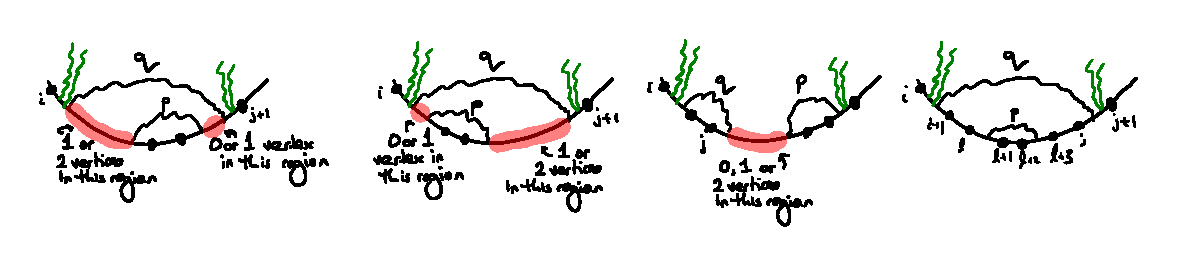
\includegraphics[scale=0.8]{3cases}
    \caption{Four cases for admissible WLDs with no unsupported vertices. The green half-propagators illustrate where propagators may occur, but are not required to exist; no other regions illustrated may support additional propagators.}\label{fig 3 cases}
  \end{figure}


In each of the four cases, when we remove the propagator labelled $p$ we obtain a diagram which satisfies the statement of the theorem by the induction hypothesis, and contains a propagator $q = (i,j)$ with no other propagators inside it (although this region may or may not contain unsupported vertices which we will call $l, l+1, \ldots$ as necessary). Call this diagram $V$ (figure \ref{fig V diagram}). 


\begin{figure}
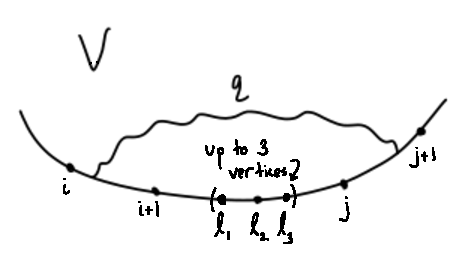
\includegraphics[scale=0.8]{Vdiagram_modified}
\caption{Diagram $V$ is $W$ with $p$ removed; there are no propagators inside $q = (i,j)$, though there may be up to 4 unsupported vertices labelled $l, l+1, \ldots$.}
\label{fig V diagram}
\end{figure}


Consider the fourth case of Figure~\ref{fig 3 cases} first, as it is the easiest.  In this case the support of $p$ is unsupported in $V$ so for every propagator $r$ in $V$ (including $q$) $J_r^{(V)} = J_r^{(W)}$.  Additionally, $J_p^{(W)}(l+a) = \{l+a\}$ for $a\in\{1,2,3\}$ and $J_p^{(W)}(l) = [n] \backslash \{l+1, l+2, l+3\}$ which proves the result in this case.


Now we proceed to consider the first three cases of Figure~\ref{fig 3 cases}.
We first describe $J_q^{(V)}(*)$: since there are no propagators inside $q$, we see from the diagram that
\[l, l+1, \ldots ,j \in J^{(V)}_q(j) \text{ (if $l$ exists) and }  j+1 \in J^{(V)}_q(j+1).\]
Note that $j+2 \not\in J^{(V)}_q(j+1)$ by Lemma~\ref{lem no fourth vertex}, so $J^{(V)}_q(j+1) = \{j+1\}$ and $j+2 \in J^{(V)}_q(i)$ by the induction hypothesis. Thus there exist vertices $d,e \in [j+2,i+1]$ with $d <e$, such that
\[J^{(V)}_q(i) = [j+2,d-1], \quad J^{(V)}_q(i+1) = [d,e-1], \quad J^{(V)}_q(j) = [e,j], \quad J^{(V)}_q(j+1) = \{j+1\},\]
and all intervals are non-empty.




We now examine what happens in each of the three cases.

%%%%%%%%%

\textbf{Left two cases}: In both of these cases, $p$ has limited effect on the Grassmann necklace of $W$ due to the presence of at least one previously unsupported vertex $l$.  Let $1\leq a\leq 3$ be the number of unsupported vertices inside $q$ in $V$; so these vertices are $l, \ldots, l+a-1$.  Write $p=(m,m+2)$ where $m\in \{i, i+1, l\}$.  Note that $l, \ldots, l+a-1$ are all in the support of $p$.  We first calculate $I^{(W)}_w$ for a starting vertex ${w \in [n]\backslash \{l, l+1, \ldots,j,j+1\}}$: if $w\in J_q^{(V)}(i)$ then
    \[
    I_w^{(W)}(r) =  \begin{cases}
        \max\{i+1, m\} & \text{if } r=p \\
        I_{w}^{(V)}(r) & \text{if } r\neq p
      \end{cases} 
    \]
    while if $w\in J_q^{(V)}(i+1)$ or $w\in J_q^{(V)}(j)$ then
    \[
    I_w^{(W)}(r) =  \begin{cases}
        l & \text{if } r=p \\
        I_{w}^{(V)}(r) & \text{if } r\neq p
      \end{cases} 
      \]
For the majority of the remaining vertices, we use the following observation: if $p$ is the first propagator to contribute to a Grassmann necklace term $I_w^{(W)}$, then the remainder of $I_w^{(W)}$ proceeds identically to the assignments of $I^{(V)}_{w+1}$.  Thus in both cases, we have for any $0\leq b <a$
    \[
    I_{l+b}^{(W)}(r) = \begin{cases}
      l+b & \text{if } r=p\\
      I_{l+b}^{(V)}(r) & \text{if } r\neq p
    \end{cases}
    \]
    If $j$ is in the support of $p$ which occurs in all cases except the second case with two vertices in the right hand region then
     \[
       I_j^{(W)}(r) = \begin{cases}
         j & \text{if $r=p$ and $j$ is in the support of $p$}\\
         I_{j+1}^{(V)}(r) & \text{if $r\neq p$ and $j$ is in the support of $p$}\\
         I_{j}^{(V)}(r) & \text{if $r\neq p$ and $j$ is not in the support of $p$}
       \end{cases}
       \]
       If $j$ is not in the support of $p$, then we must be in the second case with two vertices in the right hand region.  In this case if we start at $j$ we need to know whether propagators other than $p$ will remain around $i$ and $i+1$ when we reach vertex $i$ in the Grassmann necklace algorithm so as to know what $p$ contributes.  Consider the WLD $X$ formed from $V$ by moving the second end of $q$ to the edge $j-1$ instead of $j$.  $X$ is still admissible since we have not decreased the support of any set of propagators, so the induction hypothesis applies to it as well.  Note that $J_{j}^{(V)}(r) = J_{j}^{(X)}(r)$ for all $r\neq p$ and $J_{j}^{(X)}(r) = J_{j+1}^{(X)}(r)$ for $r\neq q,p$.  Additionally $I_{j+1}^{(X)}(q) = i$ by the induction hypothesis applied to $X$, and so starting at $j+1$ and assigning propagators to vertices according to the Grassmann necklace algorithm, when we get to the vertex $i$ in $X$ all propagators other than $q$ must have been assigned.  Starting then at $j$ in $W$ we first assign $q$ to $j$, then proceed to assign as in $X$ starting at $j+1$ and then when we get to $i$ the only propagator left to assign is $j$.  Therefore
       \[
       I_j^{(W)}(p) = m \text{ if $j$ is not in the support of $p$}
       \]
       
For the left two cases of Figure~\ref{fig 3 cases} it remains to consider the starting vertex $j+1$. If $j+1$ is in the support of $p$ then we can argue as above to get
\[
       I_{j+1}^{(W)}(r)  = \begin{cases}
         j+1 & \text{if $r=p$ and $j+1$ is in the support of $p$}\\
         I_{j+2}^{(V)}(r) & \text{if $r\neq p$ and $j+1$ is in the support of $p$}.
       \end{cases}
       \]
%Thus if $j+1$ is in the support of $p$ then $m=j-2$, the intervals $J^{(W)}_r(*)$ are still cyclic for all $r \neq p$, and
%       ***these intervals need checking***
%\[J^{(W)}_p(j-2) = [j+2,c], \quad J^{(W)}_p(j-1) = [c+1,j-1], \quad J^{(W)}_p(j) = \{j\}, \quad J^{(W)}_p(j+1) = \{j+1\}\]
%  where
%  \[
%  c = \begin{cases} d-1 & \text{if } m=i+1 \\
%    j-2 & \text{otherwise}
%      \end{cases}
%  \]
%also satisfies the statement of the theorem.

Now suppose $j+1$ is not in the support of $p$. If we start at $j+1$ we need to know whether any other propagators remain on edge $i$ when we reach vertex $i$. We already know that $J_q^{(V)}(j+1) = \{j+1\}$; in particular this means that $q$ contributes $i$ in $I_{j+2}^{(V)}$.  However the construction of $I^{(V)}_{j+1}$ first associates $q$ to $j+1$ and then proceeds identically to $I^{(V)}_{j+2}$.  In particular if $i$ was assigned in $I^{(V)}_{j+1}$, then it would not be available to assign to $q$ in $I^{(V)}_{j+2}$ as all other propagators supported at $i$ in $V$ come before $q$. 
    Therefore $p$ is the only potentially unassigned propagator on edge $i$ when we reach vertex $i$ in $W$, and
    \[
    I_{j+1}^{(W)}(r)  = \begin{cases}
      m & \text{if  $r=p$ and $j+1$ is not in the support of $p$}\\
      I_{j+1}^{(V)}(r) & \text{if  $r\neq p$ and $j+1$ is not in the support of $p$}
    \end{cases}
    \]
    
    Taking all the possibilities for the left two cases of Figure~\ref{fig 3 cases}, the intervals $J^{(W)}_r(*)$ are still cyclic for all $r \neq p$, and we can assemble the intervals for the $J_p^{(W)}(*)$ as follows.
    \begin{itemize}
      \item 
    If $m=l$ then either $a=2$ (so $l+1=m+1$, $j=m+2$, and $j+1=m+3$) or $a=3$ (so $l+1=m+1$, $l+2=m+2$, $j=m+3$, and $j+1$ is not in the support of $p$), and in both cases
    \[
    J^{(W)}_p(m) = [m+4, m], \  J^{(W)}_p(m+1) = \{m+1\}, \  J^{(W)}_p(m+2) = \{m+2\}, \  J^{(W)}_p(m+3) = \{m+3\},
    \]
    which are nonempty and otherwise as required.
  \item
        If $m=i+1$ then checking each of the three different possibilities for $a$ we likewise get
    \[
    J^{(W)}_p(m) = [m+4, d-1], \  J^{(W)}_p(m+1) = [d, m+1], \  J^{(W)}_p(m+2) = \{m+2\}, \  J^{(W)}_p(m+3) = \{m+3\},
    \]
    which are nonempty and otherwise as required.
  \item If $m=i$ then $a=1$ or $a=2$, in the former case $l=m+2$, $j=m+3$ and $j+1$ is not in the support of $p$ so
    \[
    J^{(W)}_p(m) = \{m+4\}, \  J^{(W)}_p(m+1) = [m+5, d-1], \  J^{(W)}_p(m+2) = [d, m+2], \  J^{(W)}_p(m+3) = \{m+3\},
    \]
    while in the latter $l=m+2$, $l+1=m+3$, and $j$ and $j+1$ are not in the support of $p$ so
    \[
    J^{(W)}_p(m) = [m+4, j+1], \  J^{(W)}_p(m+1) = [j+2, d-1], \  J^{(W)}_p(m+2) = [d, m+2], \  J^{(W)}_p(m+3) = \{m+3\},
    \]
    which are again as required.
    \end{itemize}

\textbf{Third case}: In this case there are no unsupported vertices $l, \ldots$ inside $q$.  Again write $p=(m, m+2)$ where $m\in \{j, j+1, j+2\}$. For $w \in [n]\backslash\{j+1,m,m+1,m+2,m+3\}$: if $w\in J_q^{(V)}(i)$ or $w\in J_q^{(V)}(i+1)$ then
    \[
    I_w^{(W)}(r) =  \begin{cases}
        m & \text{if } r=p \\
        I_{w}^{(V)}(r) & \text{if } r\neq p
      \end{cases} 
    \]
    while if $w\in J_q^{(V)}(j)$ then
    \[
    I_w^{(W)}(r) =  \begin{cases}
        \max\{m, j+1\} & \text{if } r=p \\
        I_{w}^{(V)}(r) & \text{if } r\neq p
      \end{cases} 
    \]

Finally, for $j+1$ and the vertices in the support of $p$, we have

\begin{align*}
  I_{j+1}^{(W)}(r) &= \begin{cases}
    j+1 & \text{if } r=q\\
    j+2 & \text{if } r=p\\
    I_{j+3}^{(V)}(r) & \text{if } r\neq p,q
  \end{cases}\\
  I_m^{(W)}(r) &= \begin{cases}
    m & \text{if $r=p$ and $q$ not supported on $m$}\\
    m+1 & \text{if $r=p$ and $q$ supported on $m$}\\
    I_{m}^{(V)}(r) & \text{if } r\neq p
  \end{cases}\\
  I_{m+1}^{(W)}(r) & = \begin{cases}
    m+1 & \text{if $r=p$ and $q$ not supported on $m+1$} \\
    m+2 & \text{if $r=p$ and $q$ supported on $m+1$} \\
    I_{m+1}^{(V)}(r) & \text{if } r\neq p,q
  \end{cases}\\
  I_{m+2}^{(W)}(r) & = \begin{cases}
    m+2 & \text{if } r=p \\
    I_{m+3}^{(V)}(r) & \text{if } r\neq p
  \end{cases}\\
  I_{m+3}^{(W)}(r) & = \begin{cases}
    m+3 & \text{if } r=p \\
    I_{m+4}^{(V)}(r) & \text{if } r\neq p
  \end{cases}
\end{align*}
Note that $I_{m+2}^{(V)}(r) = I_{m+3}^{(V)}(r)$ for all propagators $r$ in $V$, and that if $j+1\not\in\{m, m+1, m+2, m+3\}$ then $j+2$ and $j+3$ are unsupported in $V$ so in that case $I_{j+2}^{(V)}(r) = I_{j+3}^{(V)}(r) = I_{j+4}^{(V)}(r)$ for $r$ in $V$. Therefore, once again we can see that the $J_r^{(W)}(*)$ are cyclic for all $r$ in $V$.  Assembling the intervals for $p$ we get,
 if $m=j$ then
\[J_p^{(W)}(m) = [m+4,e-1], \  J_p^{(W)}(m+1) = [e,m], \  J_p^{(W)}(m+2) = [m+1,m+2], \  J_p^{(W)}(m+3) = \{m+3\},\]
 if $m=j+1$ then
\[J_p^{(W)}(m) = [m+4,m-1], \ J_p^{(W)}(m+1) = [m,m+1], \  J_p^{(W)}(m+2) = \{m+2\}, \  J_p^{(W)}(m+3) = \{m+3\},\]
and if $m=j+2$ then
\[J_p^{(W)}(m) = [m+4,m], \  J_p^{(W)}(m+1) = \{m+1\}, \  J_p^{(W)}(m+2) = \{m+2\}, \  J_p^{(W)}(m+3) = \{m+3\}.\]
The result now follows by induction.

%Fix $p = (i, j)$. By symmetry, we need only consider the vertices $j$, $j+1$.
%
%Let $k_1 \ldots k_r$ be the set of propagators of the form $k_x = (i_{k_x}, j)$, with $i <_{j+1} k_1 <_{j+1} \ldots k_r <_{j+1} j$. Write $k_{r+1}$ to be the counterclockwise most propagator with an end on the edge $j-1$, if it exists. If $r \geq 2$ or $r+1 = 2$, then both $P_j(p)$ and $P_{j+1}(p)$ exists for some subset of $a \in [n]$. If $r=1$ or $r+1= 2$ then only $P_j(p)$ exists. Otherwise, $P_j(p) = \emptyset$. 
%
%Consider a protecting set $P_j(p) \subset \cP$ such that $k_1 \in P_j(p)$, if it exists. Write it \bas P_j(p) = \{s_1 \ldots s_r, t_2, \ldots t_r\} \;.\eas Define $b_1 = i_{s_r}+1$. By construction, $P_j(p)$ prevents $p$ from contributing $j$ to $I_a$ for all $a \in [b_1+1, j]$. We see that, if $r >0$, for all $a \in [i+2, b_1]$, $p$ contributes $j$ to $I_a$. (\hlfix{Note that by construction, one cannot have $i_{s_r}+1 <_{j+1} i+2$.}{verify}) This is because in this range, $j$ is the first vertex of $p$ encountered by Algorithm \ref{Alg: put GN on WLD}. Furthermore, by Lemma \ref{protect conv lem}, and definition \ref{protect dfn} if $i_{s_r}+1 \not <_{j+1} i+2$ $P_1$ does not protect $p$ at $j$ for $a$ in this range. If $r = 0$ then $p$ contributes $j$ for all $a \in [i+2, j]$. In this case, we say $b_1 = j$.
%
%Now suppose $r$ is such that both $P_j(p)$ and $P_{j+1}(p)$ exists for some $a$. This time $k_2 \subset P_j(p)$. Define $b_2 = i_{s_r}+1$, where now we use $s_r$ to indicate the last propagator in this new protecting set. By construction, $P_{j+1}(p)$ prevents $p$ from contributing $j+1$ to $I_a$ for all $a \in [b_2+2, j+1]$. Therefore, if both protecting sets exist, for all $a \in [b_1+1, b_2]$ $p$ contributes $j+1$ to $I_a$. This is exactly the range in which there is exactly one valid protecting set. Therefore, in this range, $j+1$ is the first vertex of $p$ without a protective set. If there is no $a$ such that both $P_j(p)$ and $P_{j+1}(p)$ do not hold, then  $p$ contributes $j+1$ for all $a \in [b_1 +1, j+1]$.
%
%Finally, for $r > 1$, and $j_{k_2}=j$,$a \in [b2+1, j+1]$, $p$ contributes $i$ to $I_a$. Again, for all $a$ in this range, both sets $P_j(p)$ and $P_{j+1}(p)$ protect $p$ at $j$ and $j+1$ from $a$. Furthermore, by Corrollary \ref{protect cor}, there can be no protective sets of $i$ or $i+1$ in this range. 
%
%By switching the roles of $i$ and $j$, we see that for every element of $V(p)$, there is a non-empty cyclic interval such that $p$ contributes $v$ to all $I_{a}$ for in said interval.

\end{proof}


We need one more lemma before we can prove that Algorithm~\ref{alg:put GN on WLD} does in fact give the Grassmann necklace of the positroid associated to $W$.

\begin{lem}\label{lem basis as perm}
Let $W = (\cP,[n])$ be an admissible Wilson loop diagram and let $M(W)$ be its associated matroid. A subset $J \subseteq [n]$ is an independent set of $M(W)$ if and only if there exists an injective set map $f : J \rightarrow \cP$ with the property that for each $j\in J$ we have $j \in V(f(j))$.
\end{lem}

One of the most important uses of this lemma is for bases.  The lemma says that a subset $J$ of $[n]$ is a basis of $M(W)$ if and only if there is a set bijection between $J$ and $\cP$ with the property that for each $j\in J$ the propagator associated to $j$ under the bijection is supported on vertex $j$.

\begin{proof}
  Because the nonzero entries of $C(W)$ are independent indeterminants,
  $J$ is an independent set is if and only if there is some choice of $|J|$ nonzero entries of $C(W)$ one in each row associated to an element of $J$ and each in different columns.

  Each entry in $C(W)$ identifies a propagator by the row of the entry and a vertex by the column of the entry.  The entry is nonzero if and only if the propagator is supported on that vertex.
  
  Consequently, a choice of $|J|$ nonzero entries of $C(W)$ one in each row associated to an element of $J$ and each in different columns is equivalent to an assignment of the propagators of $J$ to supporting vertices so that no two are assigned to the same vertex.  Such an assignment of the propagators of $J$ to supporting vertices is exactly a map $f$ as described in the statment, hence proving the result.
\end{proof}

\begin{prop}\label{res:alg gives GN}
The sequence of $k$-subsets obtained by applying Algorithm~\ref{alg:put GN on WLD} to an admissible diagram $W$ is exactly the Grassmann necklace of the positroid associated to $W$; specifically if we let  $I_i$ be the set of labels on edge $(i,i+1)$ then the sequence $\II = (I_1, \dots, I_n)$ is the Grassmann necklace of the positroid associated to $W$.
\end{prop}

\begin{proof}
Let $I_i$ be the set of labels on edge $(i,i+1)$; the sequence $\II = (I_1, \dots, I_n)$ is a Grassmann necklace if and only if $I_{i+1} \supseteq I_i \backslash \{i\}$ for all $i \in \{1, \dots, n\}$.


Suppose for a contradition that there exists an admissible diagram for which there exists an $i$ with $k\in I_{i\backslash\{i\}}$ and $k \not\in I_{i+1}$.  Fix $n$.  Let the triple $(W, i, k)$ be such a counterexample on $n$ vertices which is minimal with respect to the number of propagators. %, and among all those counterexamples on $n$ vertices with the same number of propagators, let $(W,i,k)$ be minimal with respect to the distance from $i$ to $k$ in the $\leq _i$ order.

If $i \not\in I_i$, then there are no propagators supported on $i$ at all.  In this case it is clear that applying Algorithm~\ref{alg:put GN on WLD} at vertex $i$ and vertex $i+1$ produces exactly the same result, i.e. $I_{i+1} = I_i$, and so $(W, i, k)$ is not a counterexample at all.

Now suppose that $i \in I_i$.  Let $p$ be the propagator which contributes $i$ to $I_i$.  Either $p$ has one end on the edge $(i-1, i)$ or it has one end on the edge $(i, i+1)$.  In both cases let $(b, b+1)$ be the edge with the other end of $p$.

\textbf{case I}:  Suppose $p$ has one end on $(i-1, i)$.  Then $p$ is not supported on $i+1$, so in building $I_{i+1}$ we will take the same propagators as in the construction of $I_i$ from vertices $i+1$ up to $b-1$, that is $I_{i+1} \cap \interval{i+1}{b-1} = I_{i} \cap \interval{i+1}{b-1}$.  Furthermore, by Lemma~\ref{vertex cyclic int lem}, in building $I_{i+1}$, it must be that $p$ is taken at vertex $b$, as otherwise $b$ would never be contributed by $p$.    Consequently, in building $I_{i+1}$, when at vertex $b$ no propagator still remaining is before $p$.  This is also true in building $I_i$ when at $b$ since the same propagators have been taken beforehand.  Additionally $k\geq_i b+1$.

Let $W'$ be the diagram obtained from $W$ by removing $p$ and all propagators under it in the sense of supported between $i+1$ and $b-1$.

By the above observations when we are in $W'$ at $b$ then we are in the same situation with respect to the remaining propagators as if we began at $i$ in $W$ and moved to $b$ following the algorithm; the propagators we took in the latter case are exactly the ones removed to build $W'$.  Similarly starting at $i+1$ in $W$ and moving to $b+1$ leaves us in the same situations with respect to the remaining propagators as beginning at $b+1$ in $W'$.  This gives the equations
\begin{align*}
  I_i^W \cap \interval{b}{i-1} & = I_b^{W'} \\
  I_{i+1}^W \cap \interval{b+1}{i-1} & = I_{b+1}^{W'}
\end{align*}
where the diagram is indicated in the superscript.
Thus we have $k\in I_b^{W'}\backslash\{b\}$ and $k\not\in I_{b+1}^{W'}$ contradicting the minimality of $(W, i, k)$.

\textbf{case II}: Suppose $p$ has one end on $(i, i+1)$.  Note that by definition $p$ is the propagator contributing $i$ to $I_i$ and so it must be the first propagator in $(i, i+1)$ and hence $p$ contributes $i+1$ to $I_{i+1}$.  Observe that $k\geq_i i+2$ since $i+1\in I_{i+1}$.

Let $W'$ be the diagram obtained from $W$ just by removing $p$.  Then
\begin{align*}
  I_i^W \backslash \{i\} & = I_{i+1}^{W'} \\
  I_{i+1}^W \backslash \{i+1\} & = I_{i+2}^{W'}
\end{align*}
since in both cases in $W'$ we are simply taking the remaining propagators in the same way as we would have in $W$ after taking $p$ for the previous vertex.  Since $k \neq i+1$, we have $k\in I_{i+1}^{W'}\backslash\{i+1\}$ but $k\not\in I_{i+2}^{W'}$ contradicting the minimiality of $(W, i, k)$

%If $i \not\in I_i$, then there are no propagators supported on $i$ at all.  In this case it is clear that applying Algorithm~\ref{alg:put GN on WLD} at vertex $i$ and vertex $i+1$ produces exactly the same result, i.e. $I_{i+1} = I_i$.
%
%Now suppose that $i \in I_i$.  Order $I_i$ and $I_{i+1}$ with respect to $\leq_{i+1}$; in particular, $i$ is the last term in $I_i$ with respect to this ordering.
%
%Let $p_1$ be the rightmost propagator supported on $i$, and suppose it is removed at step $a$ with respect to vertex $i+1$.  This is the first point at which $I_{i+1}$ can differ from $I_i$, i.e. we have $I_{i+1} \cap \interval{i+1}{a-1} = I_{i} \cap \interval{i+1}{a-1}$.  If $a \not\in I_i$, then $p_1$ is the only propagator supported on $a$ at step $a$ with respect to vertex $i+1$.  All remaining steps are unchanged and we conclude that $I_{i+1} = I_i \backslash \{i\} \cup \{a\}$.
%
%If $a \in I_i$, then at step $a$ with respect to vertex $i+1$ there must be another propagator $p_2$ which lies to the left of $p_1$.  We have $I_{i+1} \cap \interval{i+1}{a} = I_i \cap \interval{i+1}{a}$, and the next possible difference
%
%{\color{red}[argh]}
%
%Although there are many different subcases to consider, the idea is always the same: we look for the first entry where $I_{i+1}$ and $I_i \backslash \{i\}$ differ (with respect to $<_{i+1}$), and show that this is the only possible difference.
%
%The reader should keep in mind that due to Proposition~\ref{res:alg k labels}, the following process cannot double back on itself.
%
%\begin{enumerate}
%\item If $p_1$ contributes $k$ to $I_{i+1}$ and $k \in I_i$, then there is another propagator $p_2$ which was deleted at step $k$ with respect to vertex $i$, but now survives at step $k$ with respect to vertex $i+1$.  All intermediate steps of the algorithm are unchanged, so $I_{i+1}$ and $I_i \backslash \{i\}$ agree up to (and including) $k$.
%\item We now look at which label $p_2$ contributes in $I_{i+1}$, and apply the same argument.  Iterate this process until we find a propagator $p_r$ which is deleted at step $j$ with respect to vertex $i+1$, but $j \not\in I_i$.
%\item $j \not\in I_i$ implies that $p_r$ is the \textit{only} propagator supported on vertex $j$ at this step.  There is therefore no knock-on effect, and any remaining propagators in the diagram contribute the same label to both $I_i$ and $I_{i+1}$. We conclude that $I_{i+1} = I_i \backslash \{i\} \cup \{j\}$.
%\end{enumerate}

\medskip

We have shown that $\II$ is a Grassmann necklace; it remains to check that this Grassmann necklace defines the positroid $\PP_W$ associated to $W$.  We need to show that:
\begin{itemize}
\item For each $i \in \interval{1}{n}$, $I_i$ is a basis for $\PP_W$.
\item If $J$ is lexicographically smaller than $I_i$ with respect to $<_i$, then $J$ is not a basis for $\PP_W$.
\end{itemize}
The algorithm is pairing each $j \in I_i$ with a unique propagator supported on that vertex so by Lemma~\ref{lem basis as perm} $I_i$ is a basis for $\PP_W$.
%%Recall from [ref] that a $k$-subset $J \in \binom{[n]}{k}$ is a basis for $\PP_W$ if and only if it has no subset $U \subseteq J$ such that $|U| > |Prop(U)|$.  It is immediately clear from the construction that $I_i$ is a basis for each $i$: the algorithm is pairing each $j \in I_i$ with a unique propagator supported on that vertex, so $|Prop(U)| \geq U$ for all $U \subseteq I_i$.

%%If $\exists l \in J$ with $Prop(l) = \emptyset$ then $J$ is clearly not a basis, so suppose otherwise.  Write
%%\[I_i = [i_1 <_i i_2 <_i \dots <_i i_r <_i \dots <_i i_k], \quad J = [i_1 <_i i_2 <_i \dots <_i j_r <_i \dots <_i j_k],\]
%%so that $I_i$ and $J$ differ for the first time in the $r$th position.  Then
%%\[r-1 \geq |Prop(\{i_1, \dots, i_{r-1}\})| = |Prop(\{i_1, \dots, i_{r+1},j_r\})|,\]
%%If $|Prop(\{i_1, \dots, i_{r-1}|\}| = r-1$ then we are done; otherwise

Suppose we have $J$ such that $J$ is a basis and yet is lexicographically less than $I_i$ with respect to $<_i$.  By Lemma~\ref{lem basis as perm} there is a set bijection between $J$ and the propagators of $W$ such that the propagator associated to $j$ is supported on vertex $j$.  Choose one such bijection.  For a propagator $p$ of $W$ write $J(p)$ for the associated $j$ according to this bijection.  Similarly write $I_i(p)$ for the vertex assigned to $p$ by the algorithm.  Since $J$ is lexicographically smaller than $I_i$, the $<_i$-smallest element of the symmetric difference of $J$ and $I_i$ is some $j_0\in J$, $j_0 \not\in I_i$.

Let $p$ be the propagator such that $J(p)=j_0$.  Since $j_0\not\in I_i$ but $p$ is supported at $j_0$, then $I_i(p) <_i j_0$.  Thus the propagator $p$ has the following property: $I_i(p) <_i J(p)$ and $I_i\cap \interval{i}{I_i(p)} = J\cap \interval{i}{I_i(p)}$.  Call this property $A$.

{}From the previous paragraph we conclude that if we ever had a $J$ which is lexicographically less than $I_i$ and yet a basis of $\PP_W$ then there exists a propagator $p$ which has property $A$.

Finally, we will prove that whenever there is a propagator $p$ which has property $A$ then there is another propagator $r$ which also has property $A$ and for which $I_i(r) <_i I_i(p)$.  Since $I_i$ is finite this would lead to infinte regress and hence is impossible and thus there can be no such $J$ which will complete the proof of the proposition.

So suppose $p$ has property $A$.  The same vertices in $\interval{i}{I_i(p)}$ are in the image of the assignment from $J$ and the image of the assignment from $I_i$ so the same number of propagators are assigned to vertices in this interval by each assignment.  However $p$ is one of the propagators assigned to a vertex in this interval in $I_i$ but not in $J$.  Thus there exists a propagator $q$ for which $J(q)\in \interval{i}{I_i(p)}$ but $I_i(q) >_i I_i(p)$.  Therefore $J(q)<_i I_i(q)$ and  $I_i\cap \interval{i}{J(q)} = J\cap \interval{i}{J(q)}$.  This is analogous to property $A$ but with the roles of $J$ and $I_i$ switched.  Thus by the same argument we must have a propagator $r$ for which $I_i(r)\in \interval{i}{J(q)}$ but $J(r)>_i J(q)$.  Therefore $r$ has property $A$ which is what we wanted to prove.

\end{proof}





In an arbitrary Grassmann necklace, it is possible for an index $i$ to appear in no terms of the Grassmann necklace (a {\em loop}) or in all terms of the necklace (a {\em coloop}). Clearly any vertex of $W$ that supports no propagators will yield a loop [ref][check: is this iff?], but with Theorem [ref][cyclic intervals thm] in hand we can now easily verify that admissible Wilson loop diagrams do not admit coloops.


\begin{cor}\label{no coloops}
Grassmann necklaces coming from admissible Wilson loop diagrams have no coloops, that is no indices $a$ such that $a \in I_i$ for all $i$.
\end{cor}
\begin{proof}
For any $a \in [n]$, $a-1$ is maximal with respect to the $<_{a}$ order. Therefore there is no propagator $p$ with $I_{a}(p) = a-1$ by Lemma~\ref{lem no fourth vertex}, i.e. $a-1 \not\in I_{a}$.
\end{proof}





\subsection{Dimension of the Wilson Loop cells}

Our next goal is to show that the dimension of the positroid cell defined by a Wilson loop diagram $(\cP, [n])$ has dimension $3|\cP|$.  Marcott in ***cite this*** has a different proof which is geometric and more elegant, bit it is not easy to track the effect of a particular propagator.  Our approach is much more explicit.


The dimension of a positroid cell is the same as the number of plusses in the associated Le diagram ***cite something***, and so with Algorithm~\ref{alg:put GN on WLD} along with the algorithm for passing from a Grassmann necklace to a Le diagram (reversing Oh's algorithm) described by some of us in \cite{reversingOh}, we can, at the cost of a bit of messy grunt work, give a recursive proof of the $3|\cP|$-dimensionality that explicitly describes the changes in the positions of the plusses in the Le diagram.

%In \cite{reversingOh}, Agarwala and Fryer give an algorithm for passing from a Grassmann Necklace to a Le diagram. We use this algorithm here to pass from a Wilson loop diagram to its associated Le diagram. In this manner, we show that the positroid cell defined by a Wilson loop diagram has dimension $3|\cP|$. Maybe say something about Amplituhedra having $4k$ dimension, but this is not quite what we have, since we are ignoring one column.
%
%When I speak of a \emph{WLD}, I mean one which satisfies your density hypothesis and other standard hypotheses.  When I speak of a propagator \emph{contributing} a vertex to an element of the Gra\ss mann\footnote{I suppose it is a bit of an affectation to use an eszett when writing in English, and actually the eszett is kind of ugly in this font, but since I've started to I'll stick with it for now but you certainly shouldn't feel obliged to do it too.} necklace I mean that according to the rule you guys have to build the Gra\ss mann necklace from the diagram by starting at a vertex and taking the clockwise-most covering propagator which hasn't already been taken, when a propagator is taken then it is contributing that vertex.  Also, I will be using your algorithm to convert the Gra\ss mann necklace into a Le diagram by non-intersecting paths.
%
%
%We need four lemmas from stuff you guys have already figured out.  The first one is a corollary of your lemma characterizing intervals contributed by each covered vertex of a
%propagator.
%
%The first lemma is Lemma~\ref{vertex cyclic int lem} and I moved it up to a previous section.
%
%The second lemma is the fact that we understand uncovered vertices.  You probably see many ways to prove this from things you already know.  One would be to say that from your algorithm the column of the uncovered vertex simply plays no role.

We need a number of lemmas, of roughly increasing degree of technicality.

\begin{lem}\label{lem uncovered}
  Let $W$ be an admissible Wilson loop diagram with $k$ propagators and with a vertex $i$ which supports no propagators.  Let $V$ be $W$ with $i$ removed.  Then the Le diagram of $W$ is the Le diagram of $V$ with an extra column of all $0$s inserted so as to be labelled $i$ on its bottom in the Oh labelling of the border of the shape of the Le diagram
\end{lem}

\note{I'm not sure how much I should assume here in terms of what the reader already knows}

\begin{proof}
  By Algorithm~\ref{alg:put GN on WLD} the Grassmann necklace of $W$ is obtained from the Grassmann necklace of $V$ by duplicating the $i$th element of the Grassmann necklace of $V$ (shifting indices as appropriate), and incrementing all indices greater than $i$ in each Grassmann necklace element.  Formally, if $I_1^{(V)}, \ldots, I_{n-1}^{(V)}$ and $I_1^{(W)}, \ldots, I_n^{(W)}$ are the Grassmann necklaces of $V$ and $W$ respectively then
  \[
  I_j^{(W)} =
  \begin{cases}
    \{\ell \in I_j^{(V)} : \ell < i\} \cup \{\ell+1 \in I_j^{(V)} : \ell \geq i\} & \text{if $j\leq i$} \\
    \{\ell \in I_{j-1}^{(V)} : \ell < i\} \cup \{\ell+1 \in I_{j-1}^{(V)} : \ell \geq i\} & \text{if $j > i$.}
  \end{cases}
  \]

  Since $i$ does not appear in the Grassmann necklace of $W$, in particular it is not in the first element of the necklace, and so in the Oh labelling of the boundary of the partition shape for the Le diagram (inside the rectangle $(k, n-k)$), $i$ labels a horizontal edge or equivalently the bottom of a column of boxes.  The shapes of the Le diagrams of $V$ and $W$ are the same except for the insertion of this column since the first Grassmann necklace elements are the same except for the incrementation of the indices $\geq i$ in the transition from the neccklace for $V$ to the necklace for $W$.

  By the algorithm of \cite{reversingOh}, since $i$ never appears in the Grassmann necklace of $W$, the column labelled $i$ is filled with all $0$s.  Otherwise the algorithm of \cite{reversingOh} behaves identically on $V$ and $W$ with the plusses for the incremented indices shifted one column to the left, thus skipping over column $i$ in the Le diagram for $W$.
\end{proof}

%The third lemma is now lemma~\ref{lem sian}.

%The fourth lemma is that we can rotate or reflect without changing the number of plusses.  The best way to see this is probably geometrically so I leave that up to you.

\begin{lem}\label{lem dihedral}
  If two Wilson loop diagrams differ by a dihedral transformation then their Le diagrams have same number of plusses.
\end{lem}

\note{Can I just cite something for this, or can one of you provide a quick geometric proof.  It would be a horrible mess to do by hand combinatorially}

%\subsubsection{Changes in Gra\ss mann necklaces for nice configurations}

%Given a propagator $p$ in a WLD $D$, note that $p$ divides remaining propagators of $D$ into two sets depending on which side of $p$ they live.

\begin{lem}\label{lem good p}
  Let $W$ be an admissible Wilson loop diagram with $n\geq 1$ propagators.  Then there is some dihedral transformation $W'$ of $W$ such that there is a propagator $p$ of $W'$ with the following properties.
  \begin{itemize}
  \item $p = (i, n-1)$ with no propagators inside it (that is $i+2, \ldots, n-2$ do not support any propagators in $W'$).
  \item Either the edges $i$ in $W'$ only supports $p$ or the edge $i$ in $W'$ supports exactly one other propagator $q = (j ,i)$ with no other propagators inside $q$.
  \end{itemize}
\end{lem}

\begin{proof}
  Remove all vertices of $W$ which do not support any propagators to get a weakly admissible Wilson loop diagram $V$.  Lemma~\ref{lem sian} applied to $V$ gives a length 2 propagator $p$ in $V$ for which either no other propagator is supported on one of the supporting edges of $p$ or there is a second length 2 propagator which is the only other propagator supported on one of the supporting edges of $p$.  Figure~\ref{fig 3 cases} shows the possible cases, and the reader can easily check that in each case $p$ must be in one of the two situations described above.

  By Lemma~\ref{lem dihedral} there is a dihedral transformation of $V$ satisfying the statement of the lemma with $p$ and $q$ both length 2.  Restoring the vertices which do not support any propagators, we obtain a dihedral transformation $W'$ of $W$ as desired (with potentially longer lengths for $p$ and $q$). 
\end{proof}

%Given an admissible Wilson loop diagram $W$, $I_i^{D}$ denotes the $i$th Grass mann necklace element corresponding to $W$.

\begin{lem}\label{lem I}
  Let $W$ be an admissible Wilson loop diagram with $n\geq 1$ propagators.  Suppose $p$ is a propagator of $W$ so that the properties of Lemma~\ref{lem good p} are satisfied for $p$ in $W$ and that $p$ has length $2$, as does $q$ if we are in the case of Lemma~\ref{lem good p} involving $q$.  Let $V$ be $W$ with $p$ removed.  Then
  \begin{align*}
    I_1^{W} & = I_1^{V} \cup \{n-3\} \\
    I_n^{W} & = I_1^{V} \cup \{n\} \\
    I_{n-1}^{W} & = I_n^{V} \cup \{n-1\} \\
    I_{n-2}^{W} & =
    \begin{cases}
      I_{n-2}^{V}\cup \{n-2\} & \text{if $n-2\not\in I_{n-2}^{V}$} \\
      I_{n-2}^{V}\cup \{n-1\} & \text{if $n-2\in I_{n-2}^{V}$, $n-1\not\in I_{n-2}^{V}$} \\
      (I_{n}^{V} - \{n-5\})\cup \{n-1,n-2\} & \text{if $n-1, n-2\in I_{n-2}^{V}$}
    \end{cases} \\
    I_{k}^{W} & =
    \begin{cases}
      I_k^{V}\cup \{n-3\} & \text{if $n-3 \not\in I_k^{V}$}\\
      I_k^{V}\cup\{n-2\} & \text{if $n-3\in I_k^{V}$}
    \end{cases} \\
    & \text{for $1<k<n-2$}
  \end{align*}
\end{lem}

\begin{figure}
 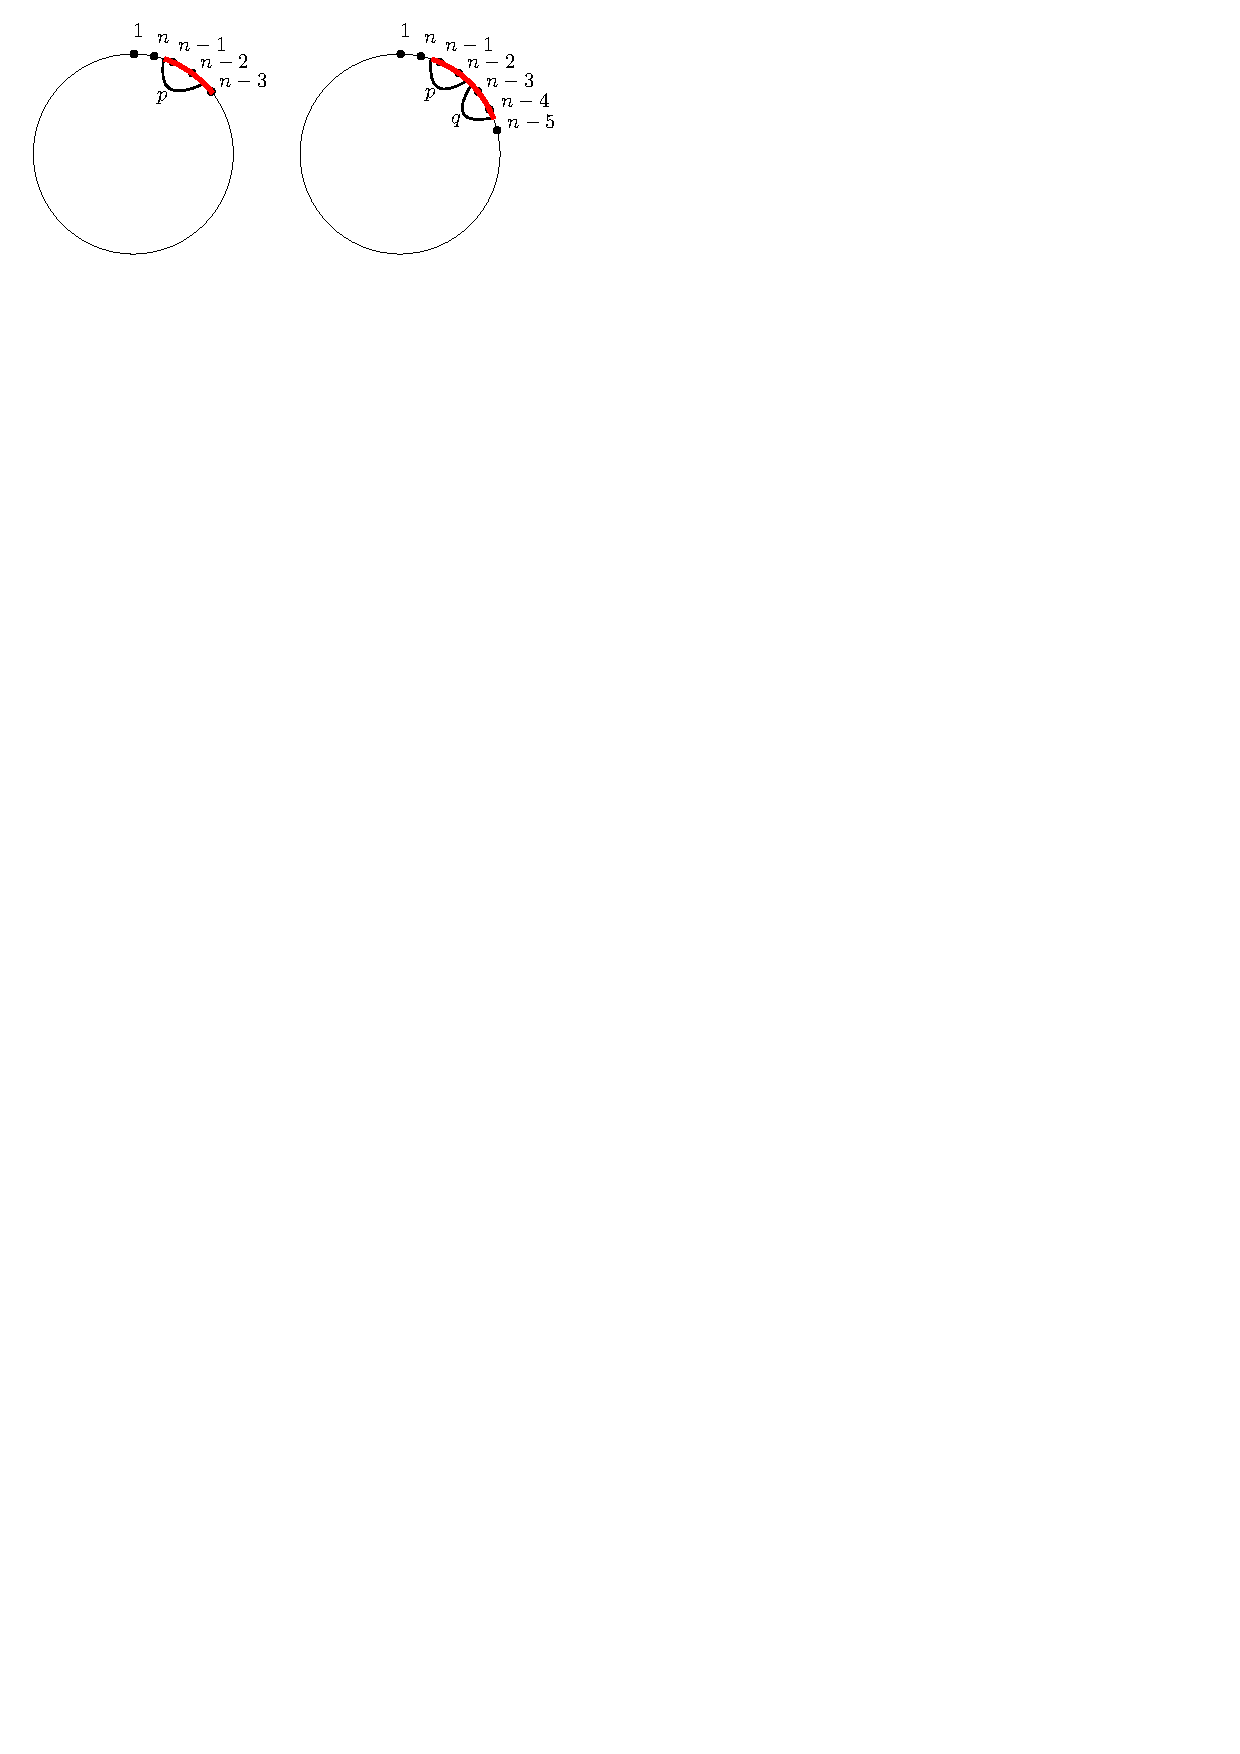
\includegraphics{specialp}
  \caption{The different possibilities for $W$ and $p$.  No other propagators can end in the fat red sections.  Other segments may have additional propagators ending in them.}\label{fig special p}
\end{figure}

\begin{proof}
  The two possible situations are illustrated in Figure~\ref{fig special p}.

  If $n-3\in I_1^{V}$ then $n-3\not\in I_1^{W}$, but then $p$ never contributes $n-3$ contradicting Lemma~\ref{vertex cyclic int lem}.  Thus $n-3\not\in I_1^{V}$ and so in building the Grassmann necklace when we get to vertex $n-3$ any other propagators of $V$ which are supported at $n-3$ have already been taken and so we take $p$.  Therefore $I_1^{W}= I_1^{V}\cup \{n-3\}$.

  In constructing $I_n^{W}$, first for vertex $n$ we take propagator $p$.  Then we are at vertex $1$ and precisely the propagators of $V$ remain.  Thus the rest of the construction will give $I_1^{V}$.  Therefore $I_n^{W} = I_1^{V}\cup \{n\}$.  Essentially the same reasoning gives $I_{n-1}^{W} = I_n^{V}\cup \{n-1\}$.

  Now consider $I_{n-2}^{W}$.  If $n-2\not\in I_{n-2}^{V}$ then at vertex $n-2$ we take $p$ and this does not affect the rest of the construction of $I_{n-2}^{V}$, so $I_{n-2}^{W} = I_{n-2}^{V}\cup \{n-2\}$.  An analogous argument takes care of the first case for $I_k^{W}$.  Suppose $n-2\in I_{n-2}^{V}$ but $n-1\not\in I_{n-2}^{V}$.  Then at vertex $n-2$ we take the same propagator in $V$ as in $W$ (in particular not $p$) because $p$ is the counterclockwisemost propagator supported on $n-2$ and so the last propagator the algorithm would choose at this vertex, and by hypothesis $n-2$ does support at least one propagator in $V$.  However, $n-1$ is not yet taken in $I_{n-2}^{V}$, so at this vertex we will take $p$ in $I_{n-2}^{W}$.  Following this the construction continues as in $I_{n-2}^{V}$.  Therefore $I_{n-2}^{W} = I_{n-2}^{V}\cup \{n-1\}$.  An analogous argument takes care of the case when we have $1<k<n-2$ and $n-3\in I_k^{V}$ but $n-2\not\in I_{k}^{V}$.  Furthermore, either $n-2$ supports no propagators in $V$ or only $q$ is supported by $n-2$ in $V$ and $q$ is also the only propagator supported by $n-3$.  Thus it is not possible for $n-3$ and $n-2$ to both be in $I_{k}^{V}$.  This means that all the cases for $I_k^{W}$ are now proved.

  The remaining case is when $n-1,n-2\in I_{n-2}^{V}$ for the construction of $I_{n-2}^{W}$.  We must then have a propagator $q$ as in the right hand side of Figure~\ref{fig special p}.  In the construction of $I_{n-2}^{W}$, at vertex $n-2$ we take propagator $q$, as in $I_{n-2}^{V}$.  Then at vertex $n-1$ we take propagator $p$ which is different from what occurs in $I_{n-2}^{V}$.  Next we are at vertex $n$ and propagators $p$ and $q$ have been taken.  Thus we are proceeding like $I_{n}^{V}$ but without propagator $q$.  Fortunately we can determine explicitely how propagator $q$ contributes to $I_{n}^{V}$.  By Lemma~\ref{vertex cyclic int lem} propagator $q$ contributes $n-5$ to $I_{n}^{V}$, and the only way this can occur is if all other propagators of $V$ were already taken by the time we got to vertex $n-5$.  Therefore $I_{n-2}^{W} = (I_{n}^{V} - \{n-5\}) \cup \{n-1, n-2\}$.  This covers all cases and hence completes the proof.
\end{proof}


\begin{lem}\label{lem shape}
  Let $V$ and $W$ be as in Lemma~\ref{lem I}.
  The shape of the Le diagram of $V$ can be built from left to right of the following blocks: a rectangle with 3 columns, one more column of the same length, a partition shape with at most as many rows as the rectangle.
  The shape of the Le diagram of $W$ can be built from left to right of the following blocks: a rectangle with 3 columns and one more row than the first rectangle of $V$, the same partition shape as in $V$.
\end{lem}

\begin{proof}
  $I_1$ determines the shape of the Le diagram.
  By Lemma~\ref{lem I}, $I_1^{W} = I_1^{V}\cup \{n-3\}$.  This implies that the right hand boundary of the shape of $V$ is the same as the right hand boundary of the shape of $W$ except that $W$ has one additional row of 3 boxes while $V$ has an additional column in the $n-3$ position; that is, a new column fourth from the left.
\end{proof}

The shapes of the Le diagrams of $V$ and $W$ are illustrated in Figure~\ref{fig Le}.  The pieces of the Le diagrams will be called $\mathcal{A}$ and $\mathcal{B}$ in what follows, as in the figure.  Over the course of the next few lemmas we will prove that the plusses in the $\mathcal{B}$ parts of the Le diagrams of $V$ and $W$ are identical and the plusses in the $\mathcal{A}$ parts are very closely related.  When we speak of a plus in the Le diagram of $V$ being the same as in $W$ or vice versa, we mean that the plus' position in $\mathcal{A}$ or $\mathcal{B}$ is the same.  Because of the column insertion the absolute indices may differ.

\begin{figure}
  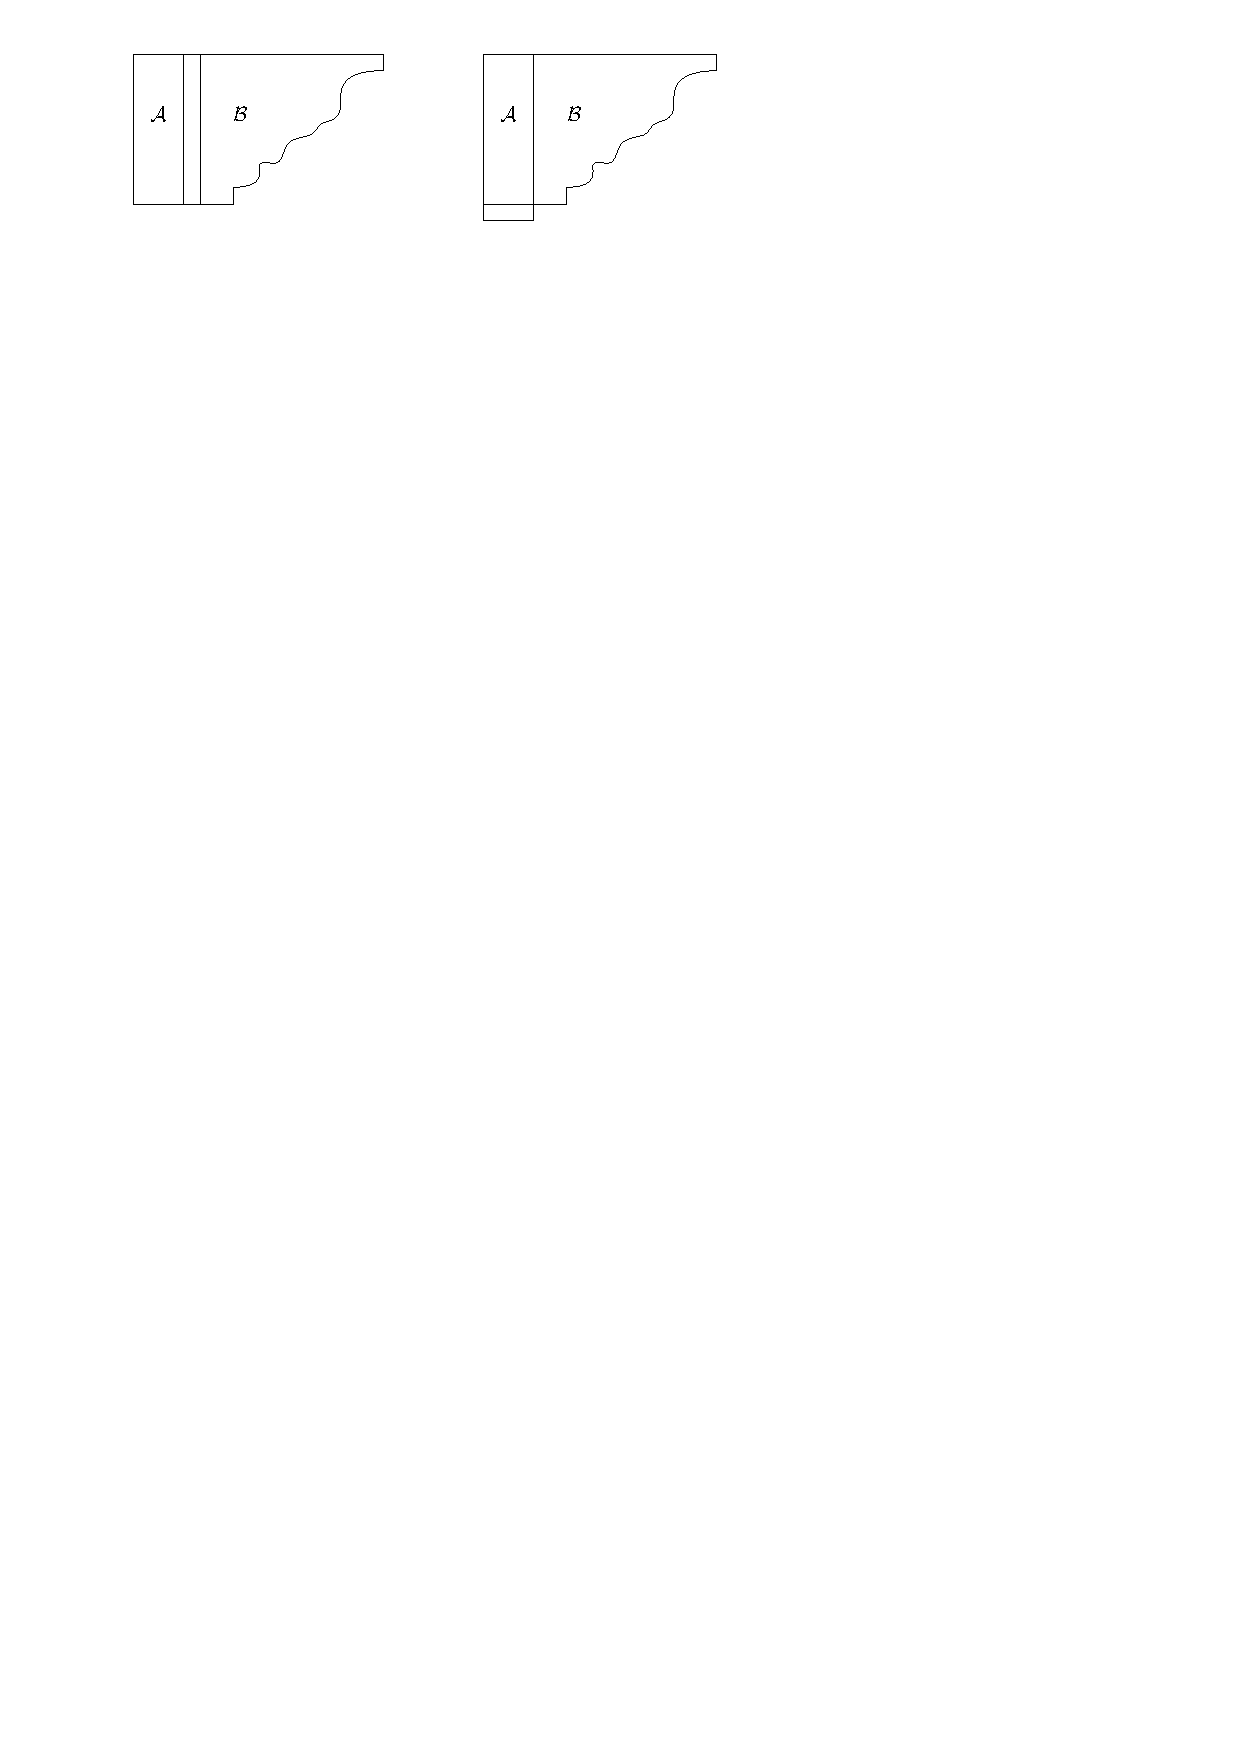
\includegraphics{Le_diagrams}
  \caption{Le diagrams for $V$ (left) and $W$ (right).}\label{fig Le}
\end{figure}

Suppose we are following the Grassmann necklace to Le diagram algorithm, and we put a plus in a box because of a path from vertical boundary edge $i$ to bottom boundary edge $j$.  Then say this plus is in the $i\rightarrow j$ position.

\begin{lem}\label{lem n and n-1}
  Let $V$ and $W$ be as in Lemma~\ref{lem I}.
  Then $I_n^{W}$ and $I_{n-1}^{W}$ give all the same plusses as $I_n^{V}$ along with plusses in the leftmost two boxes of the bottom row of the Le diagram of $W$.
\end{lem}

\begin{proof}
  By Lemma~\ref{lem I} $I_n^{W}= I_1^{V} \cup \{n\}$, so by the Grassmann necklace to Le diagram algorithm the only plus this builds in the Le diagram of $W$ is  the one in the $n-3\rightarrow n$ position, that is in the leftmost box of the bottom row.

  Also by Lemma~\ref{lem I} $I_{n-1}^{W} = I_n^{V} \cup \{n-1\}$.  Additionally $n-3\not\in I_{n}^{V}$ since if it were then $n-3$ would also be in $I_1^{V}$ and hence propagator $p$ could not contribute $n-3$ to $I_1^{W}$ in contradiction to Lemma~\ref{vertex cyclic int lem}.  Similarly $n-1, n-2\not\in I_n^{V}$.  Thus the paths putting the plusses in from $I_n^{V}$ lie completely in $\mathcal{B}$ or take some vertical boundary edge $>n-3$ to $n$.   Now view these paths in the Le diagram of $W$ and note that the path $n-3\rightarrow n-1$ is compatible, and so these paths together build the plusses that $I_{n-1}^{W}$ contributes.  That is, we get all the plusses from $I_{n}^{V}$ along with a $n-3\rightarrow n-1$ plus, that is a plus in the second to the right box of the bottom row.
\end{proof}

\begin{lem}\label{lem n-2 good}
  Let $V$ and $W$ be as in Lemma~\ref{lem I} with $n-2 \not\in I_{n-2}^{V}$.

  Then $I_{n-2}^{W}$ gives
  an $n-3\rightarrow n-2$ plus and
  all the $I_{n-1}^{V}=I_{n-2}^{V}$ plusses.
\end{lem}

\begin{proof}
  If $n-2\not\in I_{n-2}^{V}$ then $I_{n-1}^{V}=I_{n-2}^{V}$ and by Lemma~\ref{lem I} $I_{n-2}^{W} = I_{n-1}^{V} \cup \{n-2\}$.  Note that $n-3\not\in I_{n-2}^{V}$ by Lemma~\ref{vertex cyclic int lem}.  Therefore the paths for $I_{n-2}^{W}$ are the paths for $I_{n-1}^{V}$ along with the $n-3\rightarrow n-2$ path.  This gives the statement of the lemma.

\end{proof}

\begin{lem}\label{lem n-2 bad}
  Let $V$ and $W$ be as in Lemma~\ref{lem I} with $n-2,n-1 \in I_{n-2}^{V}$.

  Then $I_{n-2}^{W}$ and $I_{n-3}^{W}$ give the following plusses:
  \begin{itemize}
  \item An $n-3\rightarrow n-2$ plus and an $n-5\rightarrow n-1$ plus.
  \item All the $I_{n-1}^{V}$ plusses.
  \item $I_{n-2}^{V}$ gives an $n-5\rightarrow n-2$ plus and no other term in the Gramann necklace of $V$ gives a plus in this column.  This $+$ does not appear in $W$ from $I_{n-2}^{W}$ but an $n-5\rightarrow n-1$ plus does instead.
  \item All other plusses of $I_{n-2}^{V}$.
  \item $I_{n-3}^{V}$ gives a plus in the $n-3$ column.  This $+$ is shifted over into the $n-2$ column in $W$.
  \item All other plusses of $I_{n-3}^{V}$.
  \end{itemize}
  Furthermore, no element of the Gramann necklace of $V$ gives an $n-5\rightarrow n-1$ plus.
\end{lem}

\begin{proof}
  By Lemma~\ref{lem I} $I_{n-2}^{W}= (I_{n}^{V} - \{n-5\})\cup \{n-1,n-2\}$.  Also, by the location of $q$ in the WLD,  $n-2\not\in I_{n-3}^{V}$ and and $n-5$ is the index of the lowest vertical edge in $\mathcal{B}$.  Thus this section of the Gramann necklace of $V$ looks like
  \begin{equation}\label{eq necklace}
  I_{n-3}^{V} \underset{\substack{n-3\text{ out}\\n-2\text{ in}}}{\rightarrow} I_{n-2}^{V} \underset{\substack{n-2\text{ out}\\n-5\text{ in}}}{\rightarrow} I_{n-1}^{V} \underset{\substack{n-1\text{ out}\\\text{something in}}}{\rightarrow} I_{n}^{V} \underset{\substack{n \text{ out}\\\text{something in}}}{\rightarrow} I_1^{V}
  \end{equation}
  where the first ``something'' is either $n$ or an element of $I_1^{V}$ and the second ``something'' is an element of $I_1^{V}$.  Additionally all elements not explicitly mentioned must be in $I_1^{V}$ as they remain unchanged through this portion of the necklace.

  Using this information now determine the symmetric difference of $I_{n-2}^{V}$ and $I_1^{V}$: $n-1, n-2$ and possibly $n$ are in $I_{n-2}^{V}$ but not in $I_1^{V}$.  $n-5$ is in $I_1^{V}$ as are at least one and at most two other elements.  If there is one such element call it $a$.  If there are two call them $a$ and $b$ with $a>b$.  This means that the plusses in the Le diagram of $V$ coming from $I_{n-2}^{V}$ are as in the first part of Figure~\ref{fig messy}.  Stepping to $I_{n-1}^{V}$ simply removes the $n-5\rightarrow n-2$ path, see the second part of Figure~\ref{fig messy}.

  \begin{figure}
    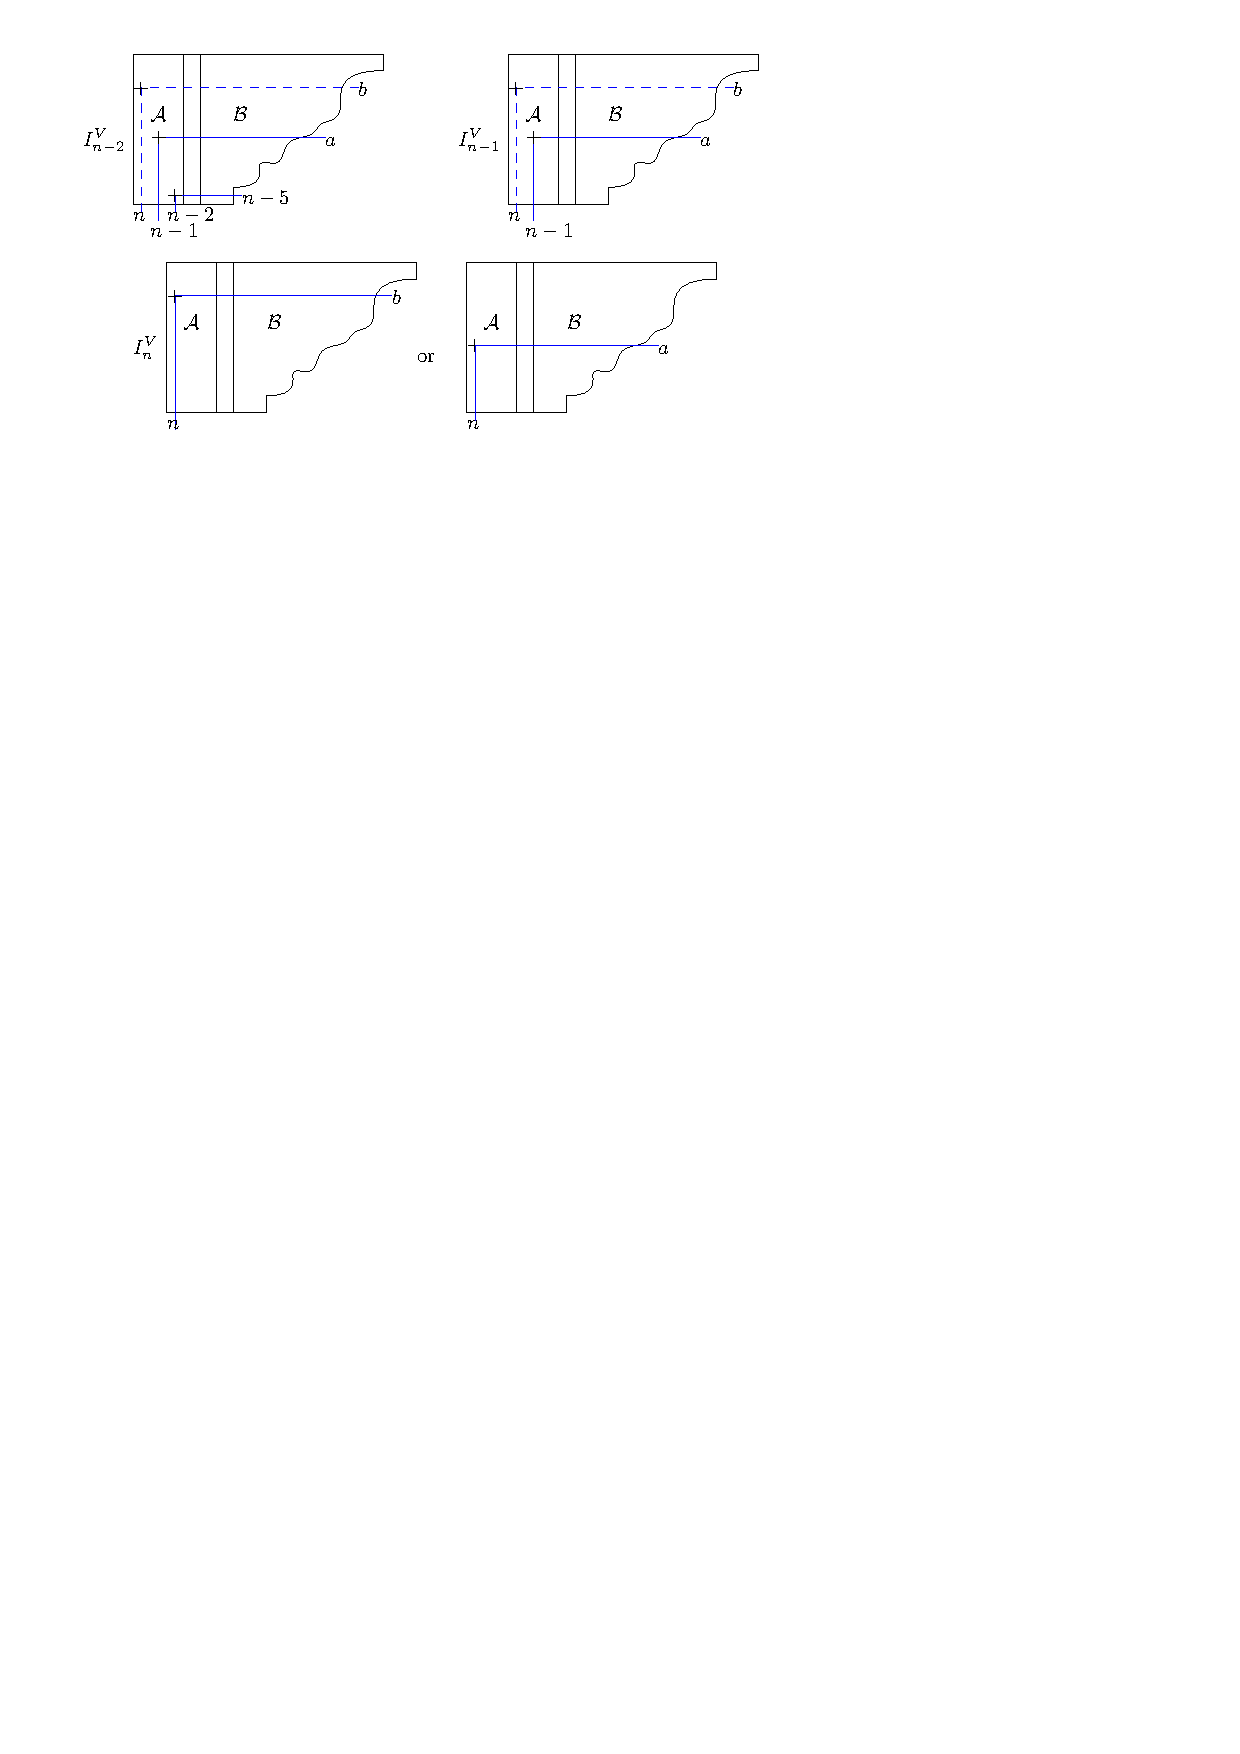
\includegraphics{messy}
    \caption{Plusses coming from $I_{n-2}^{V}$ (top left),  $I_{n-1}^{V}$ (top right) and $I_{n}^{V}$ bottom when $n-1, n-2\in I_{n-1}^{V}$.  The blue lines are the non-intersecting paths.  The dashed blue lines may or may not appear, but if one appears then they both do.}\label{fig messy}
  \end{figure}

  Stepping to $I_{n}^{V}$, $n-1$ is taken out and either $n$ is put in if it was not there before, or one of $a$ or $b$ is put in and hence no longer available as a right end for a path.  This gives two possible configurations illustrated in the bottom two parts of Figure~\ref{fig messy}.

  Now we know that $I_{n-2}^{W}  = (I_{n}^{V} - \{n-5\})\cup \{n-1,n-2\}$ so the paths for building plusses from $I_{n-2}^{W}$ go from the set $\{n-5, n-3\}$ along with whichever of $a$ and $b$ is not in $I_{n}^{V}$ to $\{n-2, n-1, n\}$.  This means that we get plusses as in Figure~\ref{fig messyD} where the left and right cases correspond to the left and right cases in the bottom parts of Figure~\ref{fig messy}

  \begin{figure}
     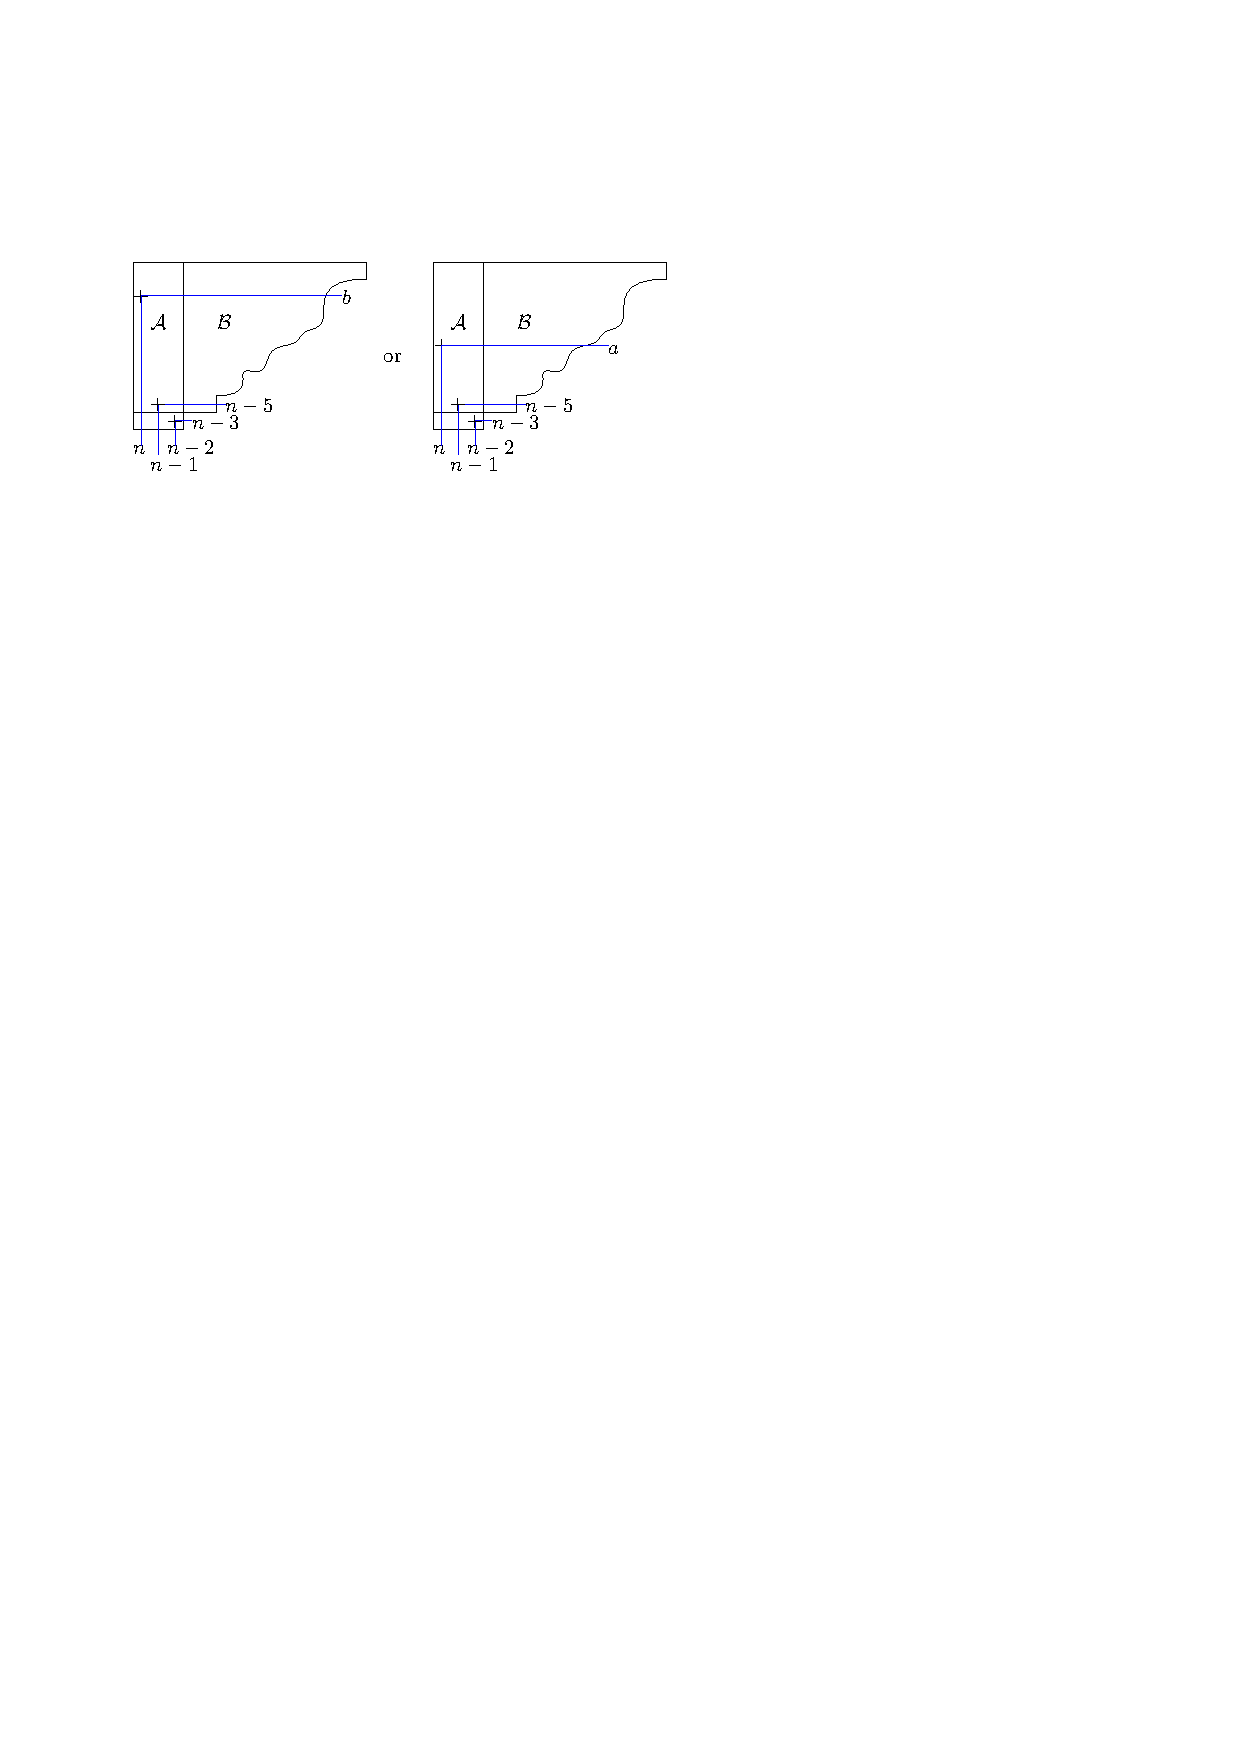
\includegraphics{messyD}
    \caption{Plusses coming from $I_{n-2}^{W}$.}\label{fig messyD}
  \end{figure}

  This proves the first item of statement of the lemma.

  Now consider $I_{n-3}^{V}$.  By \eqref{eq necklace} $I_{n-3}^{V}$ contributes the same plusses as $I_{n_2}^{V}$ except that it contributes an $n-5\rightarrow n-3$ plus in place of the $n-5\rightarrow n-2$ plus.  Also, we have $n-3\in I_{n-3}^{V}$ be the location of $q$ and so $I_{k}^{W} = I_k^{V}\cup\{n-2\}$.  Thus the paths for $I^{W}_{n-3}$ are the same as for $I^{V}_{n-3}$ except that the path that did go to $n-3$ now goes to $n-2$.  This cannot conflict with another path since \eqref{eq necklace} shows that $n-2$ only appears in $I_{n-2}^{V}$ among the necklace elements of $V$.

  Also note that $I_{n-3}^{V}, I_{n-2}^{V}$, and $I_{n-1}^{V}$ share their plusses outside of the $n-3$ and $n-2$ columns.  This proves the remaining statements of the lemma except the furthermore.

  Finally, suppose there were a $n-5\rightarrow n-1$ plus in the Le diagram of $V$.  By the algorithm, it would have to come when $n-5 \not\in I_j^{V}$.  By \eqref{eq necklace} this means that it would have to come from $I_{n-4}^{V}$, $I_{n-3}^{V}$, or $I_{n-2}^{V}$. The analysis above shows it does not come from $I_{n-3}^{V}$ or $I_{n-2}^{V}$.   Now, $n-4\in I_{n-4}^{V}$ by the location of $q$ and so $I_{n-4}^{V}$ must give an $n-5\rightarrow n-4$ plus and so cannot give an $n-5\rightarrow n-1$ plus.

\end{proof}


\begin{lem}\label{lem other k}
  Let $V$ and $W$ be as in Lemma~\ref{lem I} and take $1<k<n-2$.  Suppose that if $n-2\in I_{n-2}^{V}$ then also $n-1\in I_{n-2}^{V}$.
  Then $I_k^{W}$ gives the same plusses as $I_{k}^{V}$ except that if there is a plus in the $n-3$ column for $I_{k}^{V}$ then this plus is shifted into the $n-2$ column and no plus was already in that location.
\end{lem}

\begin{proof}
  If $n-3\not\in I_{k}^{V}$ then by Lemma~\ref{lem I} $I_{k}^{W} = I_k^{V}\cup \{n-3\}$.  Then since $n-3$ is the largest element of $I_1^{W}$ this transformation leaves the disjoint paths unchanged and so the plusses carry over from $V$ to $W$ directly.

  If $n-3\in I_{k}^{V}$ then by Lemma~\ref{lem I} $I_{k}^{W} = I_k^{V}\cup \{n-2\}$.  If $n-2$ supports no propagators in $V$ then certainly no pluses appear in the $n-2$ column of the Le diagram of $V$.  If $n-2$ supports at least one propagator in $V$ then by hypothesis so is $n-1$ and so we satisfy the hypotheses of Lemma~\ref{lem n-2 bad}.  Thus the only necklace element of $V$ containing $n-2$ is $I_{n-2}^{V}$ and this particular plus is not contributed to the Le diagram of $D$ by $I_{n-2}^{W}$.

  {}From $I_{k}^{V}$ there is a path from some vertical edge to the bottom edge $n-3$.  In $I_{k}^{W}$, $n-3$ is a vertical edge with no path and instead there must be a path to $n-2$.  By the previous paragraph no other path can end in $n-2$, so shifting the path that did go to $n-3$ to go to $n-2$ while leaving the others the same maintains non-crossingness and so must be the paths for $I_{k}^{W}$.  Thus the plus in the $n-3$ column for $C$ is shifted into the $n-2$ column, where there was no plus before, and no other plusses are changed.
\end{proof}

\begin{thm}
  The number of plusses in the Le diagram of an admissible Wilson loop diagram is three times the number of propagators.
\end{thm}

\begin{proof}
  The proof is by induction on the number of propagators.

  First note that a Wilson loop diagram $W$ with one propagator supported on vertices $i<j<k<\ell$ has Le diagram a single row with $|W|-i$ boxes.  Labelling them from left to right by $|W|, \ldots, |W|-i+1$, by the algorithm there are plusses in the $j$, $k$, and $\ell$ positions.

  Now consider Wilson loop diagrams with $k>1$ propagators.  By Lemma~\ref{lem uncovered} it suffices to prove the result for weakly admissible Wilson loop diagrams with $k$ propagators and no vertices that do not support at least one propagator.  By Lemma~\ref{lem dihedral} it suffices to prove the result for at least one Wilson loop diagram from each dihedral orbit.  Take a weakly admissible Wilson loop diagram $W$ with $k$ propagators and no vertices which do not support at least one propagator.  Make a dihedral transformation of $W$ if necessary so that $W$ has a propagator $p$ with the properties in Lemma~\ref{lem good p} relative to $W$.  If $n-1$ supports only $p$ but $n-2$ supports at least one other propagator, then flip $W$ on the line perpendicular to the edge from $n-2$ to $n-1$.  This will be our $W$ for the rest of the proof.

  Let $V$ be $W$ with $p$ removed.  Note that if $n-2$ supports at least one propagator in $V$ then so is $n-1$ by the end of the previous paragraph and so if $n-2$ supports at least one propagator in $V$ then the hypotheses of Lemma~\ref{lem n-2 bad} are satisfied.

  {}From Lemma~\ref{lem shape} we know how the shapes of the Le diagrams of $V$ and $W$ relate; let $\mathcal{A}$ and $\mathcal{B}$ be as described after that lemma.  Lemmas~\ref{lem n and n-1}, \ref{lem n-2 good}, and \ref{lem n-2 bad} tell us that the three boxes of the bottom row of the Le diagram of $W$ each have a plus.  Lemmas~\ref{lem n and n-1}, \ref{lem n-2 good}, \ref{lem n-2 bad}, and \ref{lem other k} show that there is a bijection between the plusses of the Le diagram of $V$ and the plusses of the Le diagram of $W$ that are not in the bottom row.  This bijection can be described as follows.
  \begin{itemize}
  \item Plusses from $\mathcal{B}$ for $V$ maintain their positions in $\mathcal{B}$ for $W$.
  \item Plusses from the first two columns (the $n$ and the $n-1$ columns) of $\mathcal{A}$ for $V$ maintain their positions in $\mathcal{A}$ for $W$.
  \item If there is a plus in the $n-2$ column of $\mathcal{A}$ in $V$ then Lemma~\ref{lem n-2 bad} applies, so there is exactly one such plus.  This plus maps to the $n-5\rightarrow n-1$ plus for $W$.
  \item The plusses in the $n-3$ column for $V$ shift over to the third column (the $n-2$ column) of $\mathcal{A}$ in $W$.
  \end{itemize}
  This map is clearly reversible and hence bijective except possibly for the $n-5\rightarrow n-1$ plus for $W$.   If the Le diagram of $W$ has an $n-5\rightarrow n-1$ plus then look at the Le diagram for $V$.  If the Le diagram for $V$ has a plus in the $n-2$ column then Lemma~\ref{lem n-2 bad} applies and so there is no $n-5\rightarrow n-1$ plus in the Le diagram of $V$ and the $n-5\rightarrow n-1$ plus of $W$ can be uniquely mapped to the plus in the $n-2$ column of the Le diagram of $V$.  If the Le diagram for $V$ has no plus in the $n-2$ column, then leave the $n-5\rightarrow n-1$ plus where it is in moving back to $V$.  This reverses the map.

  From all of this we get that the number of plusses in the Le diagram for $W$ is three more than the number of plusses in the Le diagram for $V$.  Applying induction completes the proof.
\end{proof}


\section{Poles of Wilson Loop Integrals}



The results of Section~\ref{sec GN algorithm} allow us to relate the position of propagators in a Wilson loop diagram $W$ to minors of $C(W)$, which we use in this section to understand the denominator of the integral $I(W)$ associated to a Wilson loop diagram (see Definition~\ref{def R(W)}). 

The main result of this section is Theorem~\ref{thm denom}, which expresses the denominator $R(W)$ in terms of the Grassmann necklace of $W$. This simplifies the computation of $R(W)$ and allows us to directly relate the poles of the integral to the combinatorics of the diagram.

We first give an algorithm which extracts the required minors from the Grassmann necklace. 


\begin{algorithm}\label{alg WLD to denom via GN}
Let $W = (\cP,n)$ be a Wilson loop diagram, and let $C(W)$ be the matrix of $W$ as defined in \eqref{C(W) dfn} (see Section~\ref{section background}).
\begin{itemize}
  \item For each $i \in [n]$, we construct a factor $r_i$ as follows:
    \begin{itemize}
      %\item Use Algorithm~\ref{alg:put GN on WLD} to obtain a bijection between the propagators and the $i-1$st Grassmann necklace element, $I_{i-1}$.  (By convention set $I_{-1}=I_n$.)  Write $I_{i-1}(p)$ for the vertex associated to propagator $p$ under this bijection.
      %\item Use Algorithm~\ref{alg:put GN on WLD} to obtain a bijection between the propagators and the $i$th Grassmann necklace element, $I_{i}$.  Write $I_{i}(p)$ for the vertex associated to propagator $p$ under this bijection.
      \item Let $S_i = \{p \in \cP \ | \ I_{i-1}(p) \neq I_i(p)\}$. (By convention, set $I_{-1} = I_n$.)
	  \item Write $\Delta_{I_i}$ for the determinant of the $k \times k$ minor of $C(W)$ with columns indexed by $I_i$.
      \item Let $r_i$ be $\Delta_{I_i}$ with all variables from rows associated to $p\not\in S_i$ set to $1$.
    \end{itemize}
  \item Define $R = \prod_{i=1}^n r_i$.
\end{itemize}
\end{algorithm}

As we take each $\Delta_{I_i}$ to simply be the determinant of a particular submatrix of $C(W)$, the overall sign of each $\Delta_{I_i}$ is well-defined.  However, we will not be interested in these signs as they only contribute an overall sign to $R$ and our main theorem in this section (Theorem~\ref{thm denom}) will simply be to show that $R$ is equal up to a $\mathbb{Q}$-multiple to the denominator of the Wilson loop diagram (see Definition~\ref{def R(W)}). 

\begin{figure}
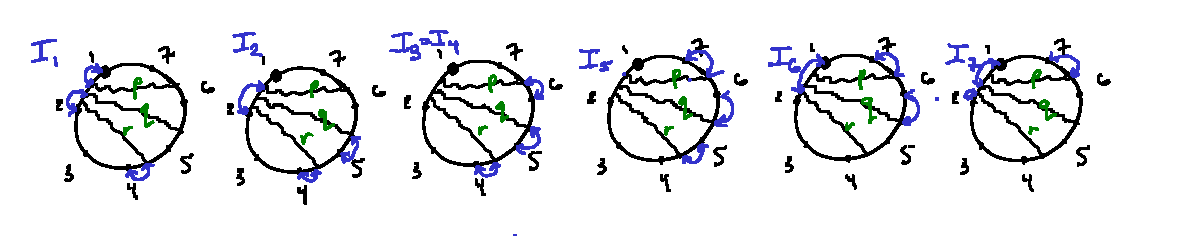
\includegraphics{egWLD_forR}
\caption{Example WLD for illustrating Algorithm~\ref{alg WLD to denom via GN} and bijections between propagators and vertices for each Grassmann necklace element.}\label{fig R eg}
\end{figure}

\begin{eg}
Consider the Wilson loop diagram in Figure~\ref{fig R eg}. Assigning propagators $p$, $q$, $s$ to rows $1,2,3$ respectively, we obtain the matrix
\[
C(W) = \begin{bmatrix} a & b & 0 & 0 & 0 & c & d \\ e & f & 0 & 0 & g & h & 0 \\ i & j & 0 & k & l & 0 & 0 \end{bmatrix}
\]
The Grassmann necklace of this diagram is 
\begin{gather*}I_1 = \{1,2,4\}, I_2 = \{2,4,5\}, I_3 = \{4,5,6\}, I_4=\{4,5,6\},\\ I_5=\{5,6,7\}, I_6 = \{6,7,1\}, I_7=\{7,1,2\}. \end{gather*}  
Figure~\ref{fig R eg} indicates the pairings between propagators and vertices for each $i \in [1,7]$.  

From $I_1$ to $I_2$, the propagators $p$ and $q$ change which vertex they are assigned to but $r$ is assigned to vertex 4 in both, so $S_2 = \{p,q\}$.  Then
\[
\Delta_{I_2}=\det\begin{bmatrix} b & 0 & 0 \\ f & 0 & g \\ j & k & l \end{bmatrix} = kgb, \qquad r_2 = \det\begin{bmatrix} b & 0 & 0 \\ f & 0 & g \\ 1 & 1 & 1 \end{bmatrix} = gb.
\]
where the 1s in the third row of the second matrix correspond to the fact that $I_1(s) = I_2(s)$.  Continuing likewise, we get $r_3 = c$, $r_4=1$ (since $I_4 = I_3$), $r_5 = lhd$, and $r_6 = i$.

At $I_7$ the situation is more complicated: we have $S_7 = \{q,s\}$, so we find that $\Delta_{I_7} = d(ej-fi)$ and $r_7 = ej-fi$. This quadratic factor corresponds to the fact that $q$ and $s$ share an edge {\em and} contribute both endpoints of that edge to $I_7$; see Proposition~\ref{prop alg gives rad} below.  

Finally, we have $r_1 = (af-be)k$.  Putting everything together, we obtain
\[
R = (af-be)kgbclhdi(ej-fi)
\]
which is squarefree and contains all factors of $\prod_{i=1}^{n}\Delta_{I_i}$. If one were to construct the denominator $R(W)$ associated to this Wilson loop diagram as per Definition~\ref{def R(W)}, we would find that (up to integer multiples) we have $R(W) = R$.
\end{eg}


\begin{prop}\label{prop alg gives rad}
  With notation as in Algorithm~\ref{alg WLD to denom via GN} and working over the field $\mathbb{Q}$ we have the following:
  \begin{enumerate}
    \item Each $\Delta_{I_i}$ is homogeneous, as is each $r_i$.
    \item Each $\Delta_{I_i}$ splits into linear and quadratic factors.  All linear factors of  $\Delta_{I_i}$ are single variables and all irreducible quadratic factors are $2\times 2$ determinants of single variables.
    \item Quadratic factors in $\Delta_{I_i}$ arise precisely when propagators $p$ and $q$ are supported on a common edge $(a,b)$ with $I_i(p)=a$ and $I_i(q)=b$.
    \item $r_i$ divides $\Delta_{I_i}$.
    \item The ideal generated by $R$ is the radical of the ideal generated by $\prod_{i=1}^{n}\Delta_{I_i}$.
  \end{enumerate}
\end{prop}

\begin{proof}
\begin{enumerate}
    \item The nonzero entries of $C(W)$ are independent indeterminates and so every $i\times i$ minor of $C(W)$ is either homogeneous of degree $i$ or is $0$.  Thus each $\Delta_{I_i}$ is homogeneous.  Furthermore, each row contributes one factor to each term in the expansion of $\Delta_{I_i}$ so the result of setting the variables from a subset of rows to $1$ is still homogeneous.  Thus each $r_i$ is homogeneous.
    \item Using the expression for the determinant as a sum over permutations we see that $\Delta_{I_i}$ is a sum over bijections between $I_i$ and $\mathcal{P}$.  The nonzero terms in this sum are precisely those bijections such that each propagator is associated to one of its supporting vertices in $I_i$, since only those locations in $C(W)$ are nonzero.  Since the nonzero entries of $C(W)$ are independent there can be no cancellation between terms in this expansion.

Suppose $\Delta_{I_i}$ has an irreducible factor $f$.  Let $\mathcal{P}'$ be the set of propagators which contribute a variable to $f$ and let $J$ be the set of vertices which contribute a variable to $f$.

The first claim is that the minor of $C(W)$ associated to $\mathcal{P}'$ and $J$ is precisely $f$.

{\em Proof of claim}: By the structure of determinants we know that $\Delta_{I_i} = fg$, where $g$ involves only variables associated to propagators not in $\mathcal{P}'$ and associated to vertices not in $J$.  

Expanding out $fg$ yields a signed sum of monomials. In each of these monomials, $f$ contributes those variables associated both to a propagator in $\mathcal{P}'$ and to a vertex in $J$, and $g$ contributes those variables associated both to a propagator not in $\mathcal{P}'$ and to a vertex not in $J$, and no other variables appear.  


Since there is no cancellation between terms, this means that the full expansion over permutations of $\Delta_{I_i}$ contains no other nonzero terms and hence no other variables.  Therefore $\Delta_{I_i}$ is equal to the determinant of the matrix obtained by taking the submatrix of $C(W)$ with columns indexed by $I_i$ and setting any variables not appearing in $\Delta_{I_i}$ to $0$.  This new matrix is, up to permutations of rows and columns, a block matrix with one block for $\mathcal{P}'$ and $J$ and the other block for the complements.  Thus its determinant, and hence also $\Delta_{I_i}$, is the product of the minors for these two blocks.  By considering which variables appear, these two factors must also be $f$ and $g$, and so in particular $f$ is the minor of $C(W)$ associated to $\mathcal{P}'$ and $J$.  This proves the claim.

A consequence of this claim is that every linear factor of $\Delta_{I_i}$ is a $1\times 1$ minor of $C(W)$, hence is a single variable, and every irreducible quadratic factor of $\Delta_{I_i}$ is a $2\times 2$ minor of $C(W)$, hence is a $2\times 2$ determinant of single variables.

All that remains is to prove that $\Delta_{I_i}$ has no irreducible factors of degree 3 or more.  Suppose for a contradiction that $f$ is a factor of $\Delta_{I_i}$ of degree $\geq 3$. Note that by removing the propagators which come before those contributing to $f$ and changing $i$ to be the first vertex which contributes to $f$, we obtain a different admissible diagram for which $f$ still divides $\Delta_{I_i}$ but also $i\in I_i$ and \note{would it be neater to note at the beginning that removing vertices which do not support any propagator has no effect so we assume there are no redundant vertices, and hence $i \in I_i$ for each $i$?  No, the point is that we can make it so that $i$ is the first index where a propagator of $f$ contributes, not just that it is in $I_i$.} $i$ contributes to $f$.  Showing that this different admissible diagram gives a contradiction is sufficient, and so we may assume that $i\in I_i$ and $i$ contributes to $f$.  Finally, we can suppose that $W$ is minimal in number of propagators with the above occuring.

Let $p$ be the propagator such that $I_i(p) = i$. There are two cases to consider, depending on which edge $p$ is supported on.  These are illustrated in Figure~\ref{fig no big factors}

\begin{figure}
  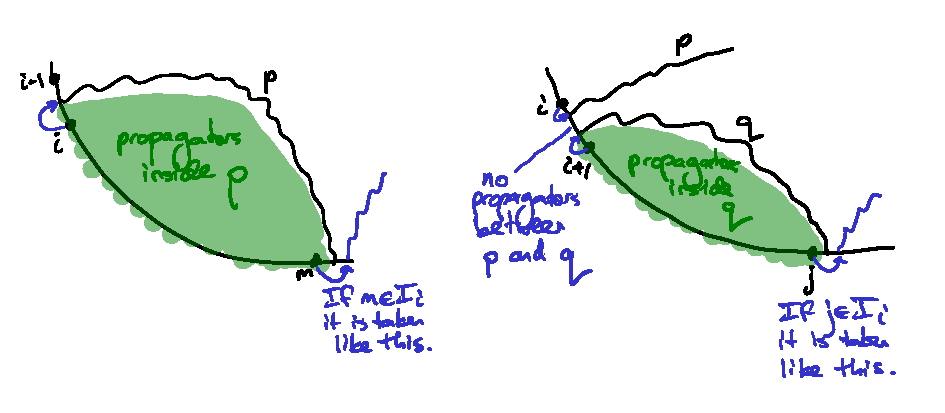
\includegraphics{no_big_factors}
  \caption{The two cases in the proof that no factors of $\Delta_{I_i}$ have degree 3 or more.}\label{fig no big factors}
\end{figure}

\textbf{Case 1}: Suppose $p$ has one end on the edge $(i-1, i)$.  Thus $p$ is supported on $(i-1, i, m, m+1)$ for some $m >_i i$, and $I_{i+1}(p) = m$ by Lemma~\ref{vertex cyclic int lem}.  

Let $S$ be the set of propagators inside $p$ along with $p$ itself. $I_i$ and $I_{i+1}$ can only differ once $p$ contributes to $I_{i+1}$, so $I_i(q) = I_{i+1}(q)$ for each $q \in S \backslash \{p\}$. Thus if a propagator contributes $m$ in $I_i$ then it must lie outside $p$.

If neither $m$ nor $m+1$ appear in $I_i$ then by Corollary~\ref{no coloops} $V(p) \cap I_i = \{i\}$, and so the row of $p$ in the matrix of $\Delta_{I_i}$ has only one nonzero entry; hence $\Delta_{I_i}$ has a linear factor contributed by $p$ and $i$, which is a contradiction.  So we must have at least one of $m$ and $m+1$ in $I_i$.  However, all propagators in $S$ are mapped by the function $I_{i}(\cdot)$ to vertices strictly before $m$, so the matrix giving $\Delta_{I_i}$ has the form
\[
\begin{bmatrix} A & B \\ 0 & C\end{bmatrix}
\]
where $A$ is the $|S|\times |S|$ matrix indexed by the propagators in $S$ and the vertices in $I_i(S)$. No other propagators can be supported on these vertices since all other propagators are outside of $p$, and $p$ is the first propagator supported at $i$; this explains the zero block.  Therefore $\Delta_{I_i} = \det A \det C$, and both factors are nontrivial since at least one of $m$ and $m+1$ appear in $I_i$.  If we remove the propagator outside of $p$ that contributes $m$ or $m+1$, we get a smaller diagram for which $\Delta_{I_i} = \det A$. This contradicts the minimality of our choices unless $\det A$ is quadratic, which in turn contradicts our assumption that $i$ and $p$ contribute to an irreducible factor $f$ of degree at least 3.

\textbf{Case 2}: Suppose $p$ has one end on the edge $(i, i+1)$.  If no other propagators are supported on $i$ then the column of $C(W)$ corresponding to vertex $i$ has only one nonzero entry in it, and so $\Delta_{I_i}$ has a linear factor contributed by $p$ and $i$; as above, this is a contradiction.  Thus we can take $q$ to be the propagator such that $I_i(q)=i+1$. We know that $q$ has one end on the edge $(i, i+1)$ and is adjacent to $p$ on that edge in the counterclockwise direction (see Figure \ref{fig no big factors}).  Write $(i, i+1, j, j+1)$ for the support of $q$.  The situation for $q$ is very similar to case 1: in particular, we have $I_{i+1}(q) = j$ by Lemma~\ref{vertex cyclic int lem} and so if $j\in I_i$ then the propagator which contributes $j$ is outside of $q$.  

Similarly to Case 1, let $S$ be the set of propagators inside $q$ along with $p$ and $q$ themselves. Then all propagators in $S$ are mapped by $I_i(\cdot)$ to vertices strictly before $j$ and no other propagators are supported on vertices strictly before $j$.  Thus the matrix giving $\Delta_{I_i}$ has the form
\[
\begin{bmatrix} A & B \\ 0 & C\end{bmatrix}
\]
where $A$ is the submatrix indexed by the propagators in $S$ and the vertices in $I_i(S)$. Again two things can now happen.  If some vertex $j$ or larger (with respect to $>_i$) belongs to $I_i$ then $B$ and $C$ are at least one column wide, and so the block form of the matrix gives a nontrivial factorization of $\Delta_{I_i}$.  This yields a contradiction as in Case 1: either $W$ contains unnecessary propagators which contradicts our minimality assumption, or $\det A$ is quadratic which contradicts the assumption that $p$ and $i$ contribute to $f$, an irreducible factor of degree at least 3.  

On the other hand, if no vertex $\geq_i j$ is in $I_i$ then $\Delta_{I_i} = \det A$.  Looking in more detail into $A$, note that the only vertices in the support of $p$ and $q$ which belong to $I_i$ are $i$ and $i+1$, and hence
\[
A = \begin{bmatrix} D & 0 \\ E & F\end{bmatrix}
\]
where $D$ is the $2\times 2$ matrix indexed by the propagators $p$ and $q$ and the vertices $i$ and $i+1$.  Thus $p$ and $i$ contribute to a quadratic factor of $\Delta_{I_i}$, once again contradicting our assumptions.

All cases have now been covered and so $\Delta_{I_i}$ has only irreducible factors of degree $2$ or less.

\item Suppose propagators $p$ and $q$ are supported on a common edge $(a,b)$, with $I_i(p)=a$ and $I_i(q)=b$.  Let $x_{p,a},x_{p,b},x_{q,a},x_{q,b}$ be the associated variables in $C(W)$. For any fixed bijection $\sigma$ from $\cP-\{p,q\}$ to $I_i -\{a,b\}$ for which each propagator is supported on its image under the bijection, we can extend $\sigma$ to a bijection of all propagators with $I_i$ in two ways: either $p\mapsto a$ and $q\mapsto b$ or $p\mapsto b$ and $q\mapsto a$.  The sum of the contributions of all these bijections to $\Delta_{I_i}$ is therefore the product of $x_{p,a}x_{q,b}-x_{p,b}x_{q,a}$ with the minor coming from $\cP-\{p, q\}$ and $I_i - \{a,b\}$.  Since there is no cancellation of terms in the expansion of $\Delta_{I_i}$, if any other terms appear then they will cause a factor which is not in the form described in the previous part.  Therefore no such terms exist and $x_{p,a}x_{q,b}-x_{p,b}x_{q,a}$ is a factor of $\Delta_{I_i}$.

Now let $f$ be a quadratic factor of $\Delta_{I_i}$.  By part (2) we know that $f$ is a $2\times 2$ minor coming from two propagators, call them $p$ and $q$, and two vertices, call them $a <_i b$.  It remains to show that $a$ and $b$ are adjacent.  From this we can conclude that $p$ and $q$ each have one end on $(a,b)$, as any other way for both $p$ and $q$ to be supported on two consecutive vertices would contradict noncrossing or the density requirement of admissibility.

As in the proof of part (2), make a new admissible diagram by removing the propagators which come before $f$ and set $i=a$.  The cases in the proof of part (2) show how $\Delta_{I_i}$ factors: in particular the vertices supporting the other end of $p$ either do not appear in $I_i$, or they contribute to a different factor of $\Delta_{I_i}$ than $p$ and $a$ do.  By assumption $b$ contributes to the same factor as $a$.  Therefore $(a,b)$ is an edge.

\item Consider $p\in S_i$, and note that $\Delta_{I_i}$ is homogeneous linear in the variables of the row corresponding to $p$.  By part (2), either exactly one variable in the row corresponding to $p$ appears in $\Delta_{I_i}$ and this variable is a factor of $\Delta_{I_i}$, or exactly two variables from the row corresponding to $p$ appear in $\Delta_{I_i}$ and they appear as part of a quadratic factor.  In the first case let the variable be $x$, then $x$ is a factor of both $r_i$ and $\Delta_{I_i}$ and is the only variable from this row in either polynomial.  

Now suppose two variables from the row $p$ appear in a quadratic factor $f$.  By part (3), there is another propagator $q$ and an edge $(a,b)$ such that $f$ is the $2\times 2$ minor coming from $p, q$ and $a, b$, with $I_i(p)=a$, $I_i(q)=b$.  There are two situations which can occur, both illustrated in Figure~\ref{fig quadratic}; we show that in both cases it follows that $q \in S_i$ as well.

\begin{figure}
  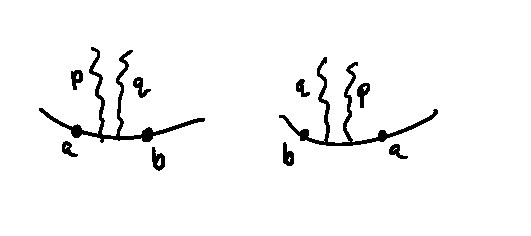
\includegraphics{quadratic}
  \caption{The situations giving a quadratic factor with variables appearing in $r_i$.}\label{fig quadratic}
\end{figure}

In both cases, since $I_{i-1}(p)\neq a$ by assumption it follows from Lemma~\ref{vertex cyclic int lem} that $I_{i-1}(p) <_{i-1} a$ and no other vertex supporting $p$ lies between $I_{i-1}(p)$ and $a$. In the case that $b<_i a$ and $q$ is taken before $p$ in $I_i$, this means that $I_{i-1}(p)=b$ and so $I_{i-1}(q)\neq b$.  Thus $q\in S_i$ and so $f$ is a factor of $r_i$.

Now consider the case where $a<_i b$, and suppose for contradiction that $q \not\in S_i$, i.e. that $I_{i-1}(q) = b$. Since $I_{i-1}(p) \neq a$, there must be some other propagator $s$ with $I_{i-1}(s) = a$ (else $I_{i-1}$ assigns $q$ to $a$). This propagator cannot lie on edge $(a,b)$ since by Lemma~\ref{vertex cyclic int lem} we must have $I_i(s) = a$ or $b$, contradicting the fact that $I_i(p) = a$ and $I_i(q) = b$; thus $s$ has an end on $(a-1,a)$ and is inside $p$ from the point of view of $i-1$.

Say $s$ is supported on $(j, j+1, a-1, a)$ and $p$ is supported on $(k, k+1, a, b)$ with $i-1 \leq_{i-1} k+1 \leq_{i-1} j+1$. But by Lemma~\ref{lem no fourth vertex}, if $I_{i-1}(s) = a$ then $a$ cannot be maximal in the support of $s$ with respect to $<_{i-1}$; thus we must have $i-1 = j+1$, and we are in the situation in figure~\ref{fig part 4}.

\begin{figure}
  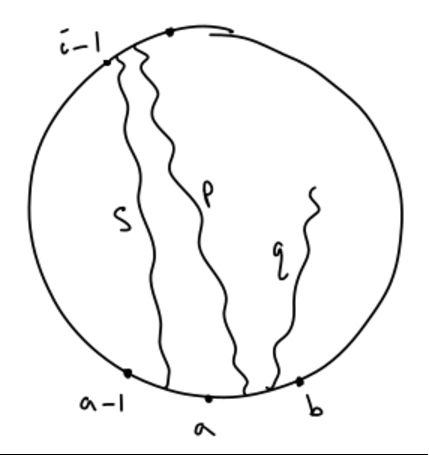
\includegraphics[scale=0.5]{part4}
  \caption{In order to obtain $I_{i-1}(s) = a$, propagators $s$ and $p$ must each have an end on the edge $(i-2,i-1)$.}\label{fig part 4}
\end{figure}

Since $p$ changed its association from $I_{i-1}$ to $I_i$, we have $I_{i-1}(p) = i-1$ by Lemma~\ref{vertex cyclic int lem}. From figure~\ref{fig part 4} it follows that $I_{i-1}$ assigns $p$ to $i-1$ and then proceeds identically to $I_i$ for all vertices inside $p$, implying that $I_{i-1}(s) = I_i(s)$. Since $I_{i-1}(s) = a$ and $I_i(s) \neq a$, this is a contradiction. 

Thus $q\in S_i$ after all, and so again $f$ is a factor of $r_i$ as required.

  

% Thus $s$ is supported on $a$ but does not have an edge on $(a,b)$ and so $s$ must have an end on $(a-1, a)$ and so be inside $p$ from the point of view of $i-1$.  Say $s$ is supported on $(j, j+1, a-1, a)$ and $p$ is supported on $(k, k+1, a, b)$ with $i-1 \leq_{i-1} k+1 \leq_{i-1} j+1$.  Again by Lemma~\ref{lem susama}, immediately after $s$ contributes $a$ it must contribute $j$ and so $I_i(s)=j$.

% Finally we want to show $I_i(s)=j$ gives a contradiction.  If $k=j$ then $I_{i}(s)= k$, but $p$ has not yet been taken as $I_i(p)=a$ and $p$ comes before $s$ around $k$, so this is a contradiction.  If $k+1=j$ then similarly $I_{i}(s)=k+1$ and yet $p$ comes before $s$ around $k$, a contradiction to $I_i(p)=a$.  Now suppose $k+1 <_{i-1} j$ then we have $i-1 \leq_{i-1} k+1 <_{i-1} I_i(s) = j$ so $i\leq_{i} I_i(s)$ which gives that
% \[
% I_i(s) <_i I_{i-1}(s) \qquad \text{and} \qquad I_i(s) <_{i-1} I_{i-1}(s)
% \]
% \note{Is this known to be impossible by the proof sketch of Lemma~\ref{lem susama} that you emailed or something similar.  I'm thinking this proof is already too long and the fact that this is impossible would be better as a lemma.}

\item If $W$ has zero propagators then all $I_i=\emptyset$ and both $R$ and $\prod_{i=1}^n \Delta_{I_i}$ are equal to $1$, so the result holds in this case.  Now assume $W$ has at least one propagator.

First we show that every factor of $\prod_{i=1}^n \Delta_{I_i}$ divides $R$.  Take an irreducible factor $f$ of $\prod_{i=1}^n \Delta_{I_i}$. There exists some $i$ such that $f|\Delta_{I_i}$ but $f\!\!\nmid\!\! \Delta_{I_{i-1}}$, since otherwise the variables corresponding to the propagators contributing to $f$ which do not themselves appear in $f$ could never appear, contradicting Lemma~\ref{vertex cyclic int lem}.  If $f$ is a linear factor, say from associating propagator $p$ to vertex $a$, then $I_{i}(p)=a$ and $I_{i-1}(p)\neq a$ so this factor appears in $r_i$.  If $f$ is a quadratic factor, say from associating propagators $p$ and $q$ to vertices $a$ and $b$ respectively, then again we cannot have both $I_{i-1}(p) = a$ and $I_{i-1}(q) = b$, else $f$ divides $\Delta_{i-1}$. However, by the proof of part (4), if one of $p,q$ belongs to $S_i$ then the other does as well.  Thus $f$ divides $r_i$.

Next we need to show that $R$ is squarefree.  Suppose $f^2|R$.  If $f$ is a linear factor, say from associating propagator $p$ to vertex $a$, then there must be two distinct points in the Grassmann necklace algorithm where $p$ changes from not being associated to vertex $a$ to being associated to vertex $a$.  This contradicts Lemma~\ref{vertex cyclic int lem}.  Now suppose $f$ is a quadratic factor, say from propagators $p$ and $q$ supported on the edge $(a, b)$ with $p$ before $q$ on the edge.  In this case it is not possible for any $I_i$ to associate $p$ to $b$ and $q$ to $a$.  Furthermore, we know by part (4) that $p$ changes from not being associated to $a$ to being associated to $a$ if and only if $q$ changes from not being associated to $b$ to being associated to $b$.  Thus $f^2|R$ implies that twice in the Grassmann necklace $p$ must change from not being associated to vertex $a$ to being associated to vertex $a$. This is again a contradiction, and so $R$ is squarefree.

Taking everything together we have that $R|\prod_{i=1}^n \Delta_{I_i}$, $R$ contains all factors of $\prod_{i=1}^n \Delta_{I_i}$ and $R$ is squarefree.  Therefore the ideal generated by $R$ is the radical of the ideal generated by $\prod_{i=1}^n \Delta_{I_i}$.
  \end{enumerate}
\end{proof}


\begin{thm}\label{thm denom}
Given any admissible Wilson loop diagram $W$, let $\{I_1, \ldots I_n\}$ be the associated Grasmann necklace. Then the denominator of the integral, $R(W)$ (see Definition~\ref{def R(W)}), is a $\mathbb{Q}$-multiple of the radical of $\prod_{i=1}^n \Delta_{I_i}$, where $\Delta_{I_i}$ is the determinant of the $k \times k$ minor indicated by $I_i$.  Equivalently, $R(W)$ is a $\mathbb{Q}$-multiple of the $R$ of Algorithm~\ref{alg WLD to denom via GN}.
\end{thm}

\begin{proof}
The equivalence of the final statement of the theorem is due to Proposition~\ref{prop alg gives rad}.  It remains to prove that $R(W)$ is an integer multiple of the $R$ of Algorithm~\ref{alg WLD to denom via GN}.

To this end, first note that $R(W)$ and $R$ both have total degree $4|\mathcal{P}|$; the degree of $R(W)$ is immediate from the definition while that of $R$ follows from Lemma~\ref{vertex cyclic int lem}.  By Proposition~\ref{prop alg gives rad} every factor of $R$ is either a single variable or a quadratic factor coming from two propagators supported on a common edge.  The factors of each $R_e$ making up $R(W)$ in the notation of Definition~\ref{def R(W)} are all of this form and hence every factor of $R$ divides $R(W)$.
Finally, since $R$ is squarefree, this implies that $R(W)$ is a $\mathbb{Q}$-multiple of $R$.
\end{proof}

\note{Is there any point in working out the $\mathbb{Q}$-coefficient, or otherwise discussing the field?}

***explain why this result was interesting***


\end{document}
